\documentclass{article}
\usepackage[utf8]{inputenc}
\usepackage{authblk}
\usepackage{setspace}
\usepackage[margin=1.25in]{geometry}
\usepackage{graphicx}
% \graphicspath{ {./figures/} }
\graphicspath{ {../figures/} }
\usepackage{subcaption}
\usepackage{amsmath}
\usepackage{lineno}
% \linenumbers

\usepackage{enumerate}
\DeclareMathOperator{\diag}{diag}
\usepackage{multirow}
\usepackage{booktabs}
\usepackage{footnote}
\usepackage{bm}
\usepackage[ruled,linesnumbered]{algorithm2e}
\setcounter{MaxMatrixCols}{20}
\usepackage{tikz}
\usetikzlibrary{arrows.meta, calc, fit, positioning, quotes, graphs, shapes.geometric}
\def\T{\mathrm{T}}

\usepackage[final]{changes}
% \usepackage[defaultcolor=red]{changes}
% \added{xxx}
% \deleted{xxxx}
% \replaced{a}{b}

%%%%%% Bibliography %%%%%%
% Replace "sample" in the \addbibresource line below with the name of your .bib file.
\usepackage[style=nejm, citestyle=numeric-comp, sorting=none]{biblatex}
\addbibresource{SST_main.bib}

%%%%%% Title %%%%%%
% Full titles can be a maximum of 100 characters, including spaces. 
% Title Format: Use title case, capitalizing the first letter of each word, except for certain small words, such as articles and short prepositions
\title{Maximum Allowable Current Determination of RBS By Using a Directed Graph Model and Greedy Algorithm}

%%%%%% Authors %%%%%%
% Authors should be listed in order of contribution to the paper, by first name, then middle initial (if any), followed by last name.
% Authors should be listed in the order in which they will appear in the published version if the manuscript is accepted. 
% Use an asterisk (*) to identify the corresponding author, and be sure to include that person’s e-mail address. Use symbols (in this order: †, ‡, §, ||, ¶, #, ††, ‡‡, etc.) for author notes, such as present addresses, “These authors contributed equally to this work” notations, and similar information.
% You can include group authors, but please include a list of the actual authors (the group members) in the Supplementary Materials.
\author[1]{30577}
% \author[1$\dag$]{Binghui Xu}
% \author[1$\dag$]{Guangbin Hua}
% \author[1*]{Cheng Qian}
% \author[1,2]{Quan Xia}
% \author[1]{Bo Sun}
% \author[1]{Yi Ren}
% \author[1]{Zili Wang}

%%%%%% Affiliations %%%%%%
% \affil[1]{School of Reliability and Systems Engineering, Beihang University, Beijing, 100191, China}
% \affil[2]{School of Aeronautic Science and Engineering at Beihang University, Beijing, China}
% \affil[*]{Address correspondence to: cqian@buaa.edu.cn}
% \affil[$\dag$]{These authors contributed equally to this work.}

%%%%%% Date %%%%%%
% Date is optional
\date{}

%%%%%% Spacing %%%%%%
% Use paragraph spacing of 1.5 or 2 (for double spacing, use command \doublespacing)
\onehalfspacing

\begin{document}

\maketitle

%%%%%% Abstract %%%%%%
\begin{abstract}
Reconfigurable Battery Systems (RBSs) present a promising alternative to traditional battery systems due to their flexible and dynamically changeable topological structure subjected to battery charging and discharging strategies.
During the operation of the RBS, the Maximum Allowable Current (MAC) of system that ensures each battery's current remains within a safe range, is a critical indicator to guide the system's reconfiguring control, ensuring its safety and reliability. 
In this paper, we firstly propose a calculation method for the MAC of arbitrary RBS using a greedy algorithm in conjunction with a directed graph model of the RBS.
\added{
By introducing the shortest path of the battery, the greedy algorithm transforms the enumeration of switch states in the brute force algorithm into the combination of the shortest paths, which greatly increases the efficiency of the determination of the MAC.
The directed graph model, based on the equivalent circuit, provides a specific method for calculating the MAC of a given structure.
This method has been validated on two published 4-battery-RBSs and one with more complex structure.
It obtaining the same results as the brute force algorithm method, while achieves significantly improved computational efficiency ($N_s 2^{N_s - N_b} \log N_b$ times faster than the brute force algorithm for a RBS with $N_b$ batteries and $N_s$ switches, theoretically).
The main advantage of this method is its ability to calculate the MAC of RBSs with arbitrary structures, even in the scenarios with random isolated batteries.
}
\deleted{
In this method, a new directed graph model is developed to model the structure of RBS, and a greedy algorithm is designed to find the possible circuit that enable MAC.
Then, the MAC is calculated based on the circuit in-cooperate with the equivalent model of batteries and switches. 
The effectiveness of the proposed method is validated by a novel and complex RBS structure. 
The results show that this method is capable to calculated the MAC of RBSs with different structures or different battery sizes efficiently, which proves the correctness of this method and its potential in facilitating next-generation RBS designs and applications, including battery isolation.
}
\end{abstract}

%%%%%% Main Text %%%%%%

\section{Introduction}

Battery Energy Storage Systems (BESSs) are extensively employed in various applications, such as wind power plants and space power systems, to store and release high-quality electrical energy \cite{desiqueiraControlStrategySmooth2021,yangBatteryEnergyStorage2018,choCommercialResearchBattery2015,zhangDevelopmentProspectChinese2021,schwanbeckInternationalSpaceStation2019}.
Typically, a BESS consists of numerous batteries interconnected by series-parallel circuitry to provide the required capacity storage.
However, traditional BESSs, in which the batteries are connected in a fixed topology, exhibit a significant weakness in their worst battery due to the so-called cask effect.
Moreover, if this worst battery fails \replaced{from}{during} operation, it can exacerbate the degradation of other batteries with a high possibility, leading to reliability and safety issues \cite{yangUnbalancedDischargingAging2016,fengPropagationMechanismsDiagnosis2019,jeevarajanBatterySafetyQualifications2012}.
These problems have become significant technical barriers in the development of new-generation space vehicles \replaced{unfortunately}{and urgently need to be addressed} \cite{pomboHybridPowerSystem2021}.


Reconfigurable Battery System (RBS), which can dynamically switch to different circuit topology configurations as required, is expected to solve the above problems\cite{hanNextGenerationBatteryManagement2020a}.
The ability of switching circuit helps to isolate unhealthy batteries, \replaced{thereby improving}{and thereby improve} the safety and reliability of the battery system.
\replaced{In order to illustrate the working principle of RBS, a typical RBS structure developed by Visairo \cite{visairoReconfigurableBatteryPack2008}(Figure \ref{fig:stru-Visairo}) is taken as an example to show the reconfiguration process.}{Figure \ref{fig:stru-Visairo} shows a typical RBS structure developed by Visairo \cite{visairoReconfigurableBatteryPack2008} for dynamically adjusting the output voltage and current.}
In this structure, the batteries can be connected not only in series when the switches $S_1$, $S_5$, $S_6$, $S_7$, $S_8$, $S_9$, and $S_{13}$ are closed (Figure \ref{fig:stru-Visairo-serial}), but also in parallel when $S_1$, $S_2$, $S_3$, $S_4$, $S_5$, $S_9$, $S_{10}$, $S_{11}$, $S_{12}$, and $S_{13}$ are closed (Figure \ref{fig:stru-Visairo-parallel}).
Furthermore, when an unhealthy battery, for instance the orange one $B_3$ in Figure \ref{fig:stru-Visairo-isolate}, appears in the RBS, it can be isolated by opening its two adjacent switches (i.e. $S_4$ and $S_{11}$), ensuring the system still remains a reliable working mode.

\begin{figure}[htbp]
    \centering
    \begin{subfigure}[b]{0.45\textwidth}
        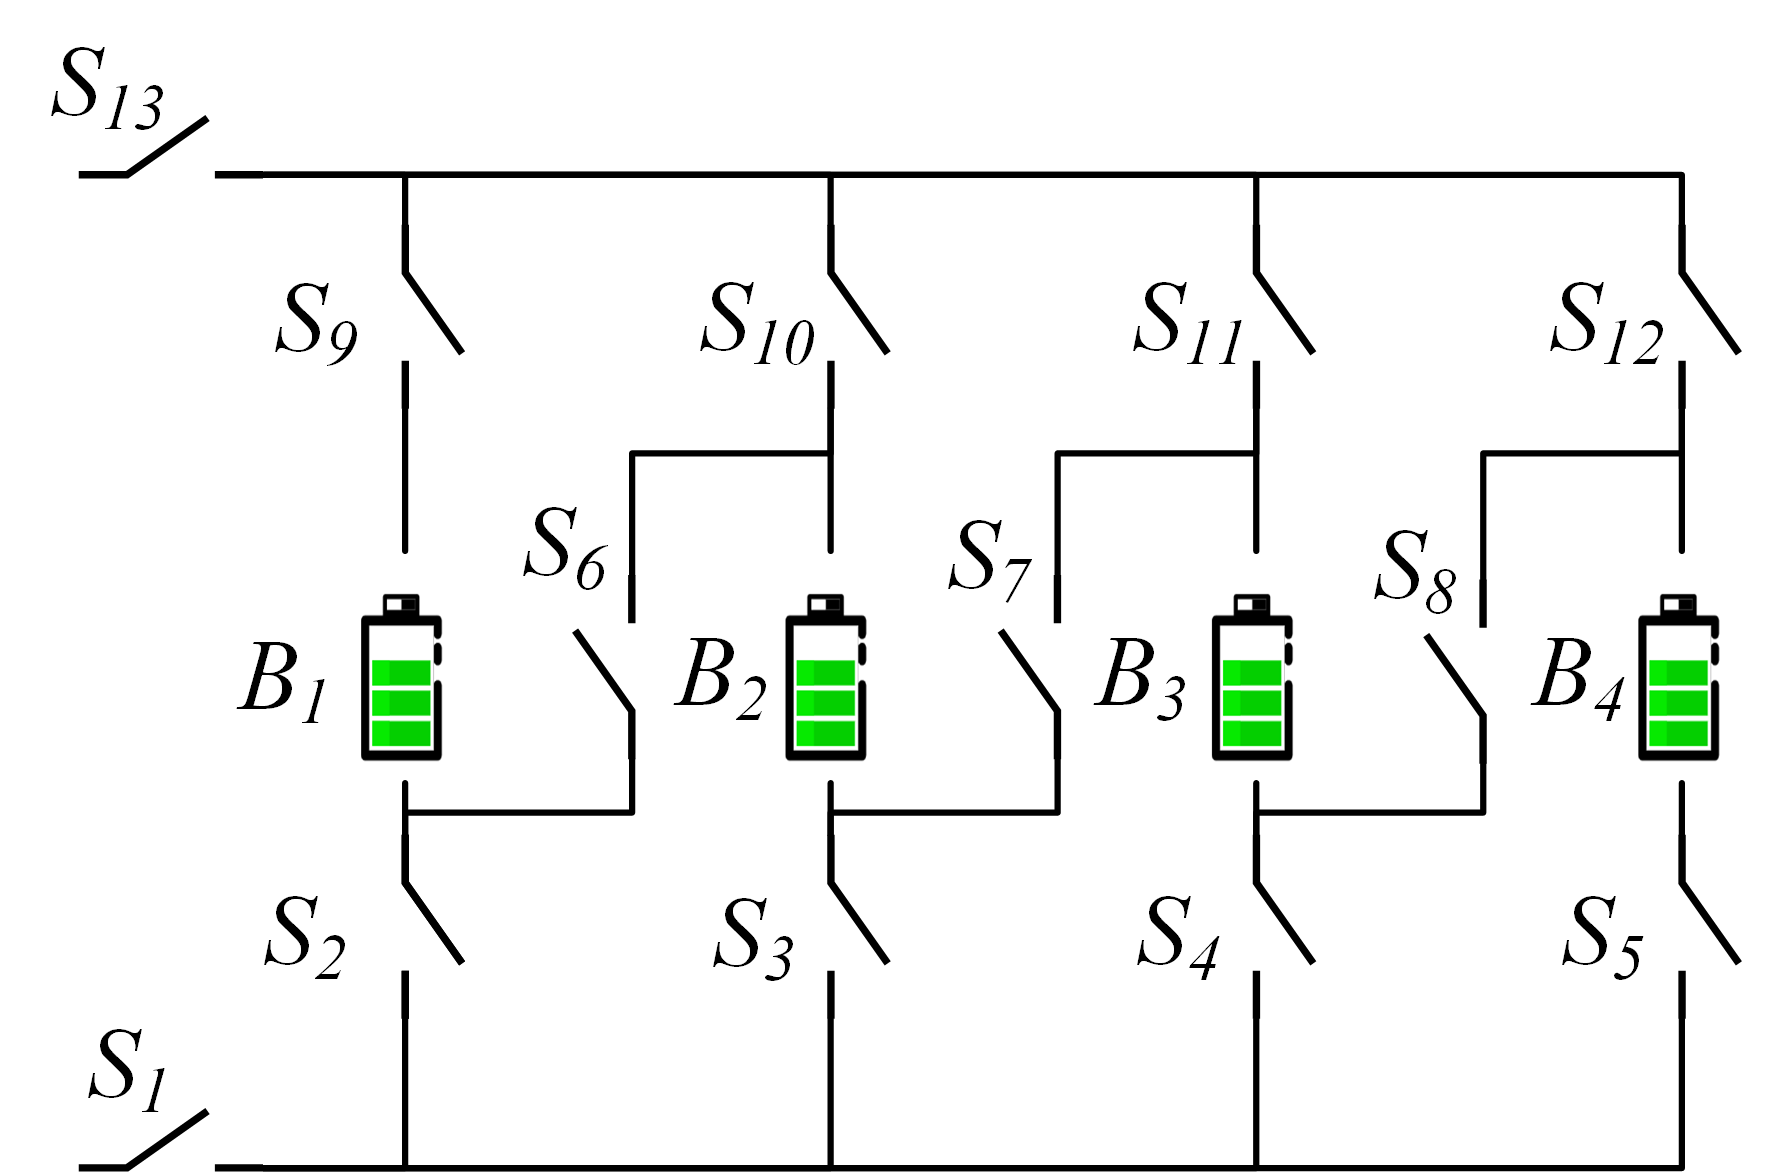
\includegraphics[width=\textwidth]{stru-V-origin.png}
        \caption{}
        \label{fig:stru-Visairo}
    \end{subfigure}
    \hspace{0.05\textwidth}
    \begin{subfigure}[b]{0.45\textwidth}
        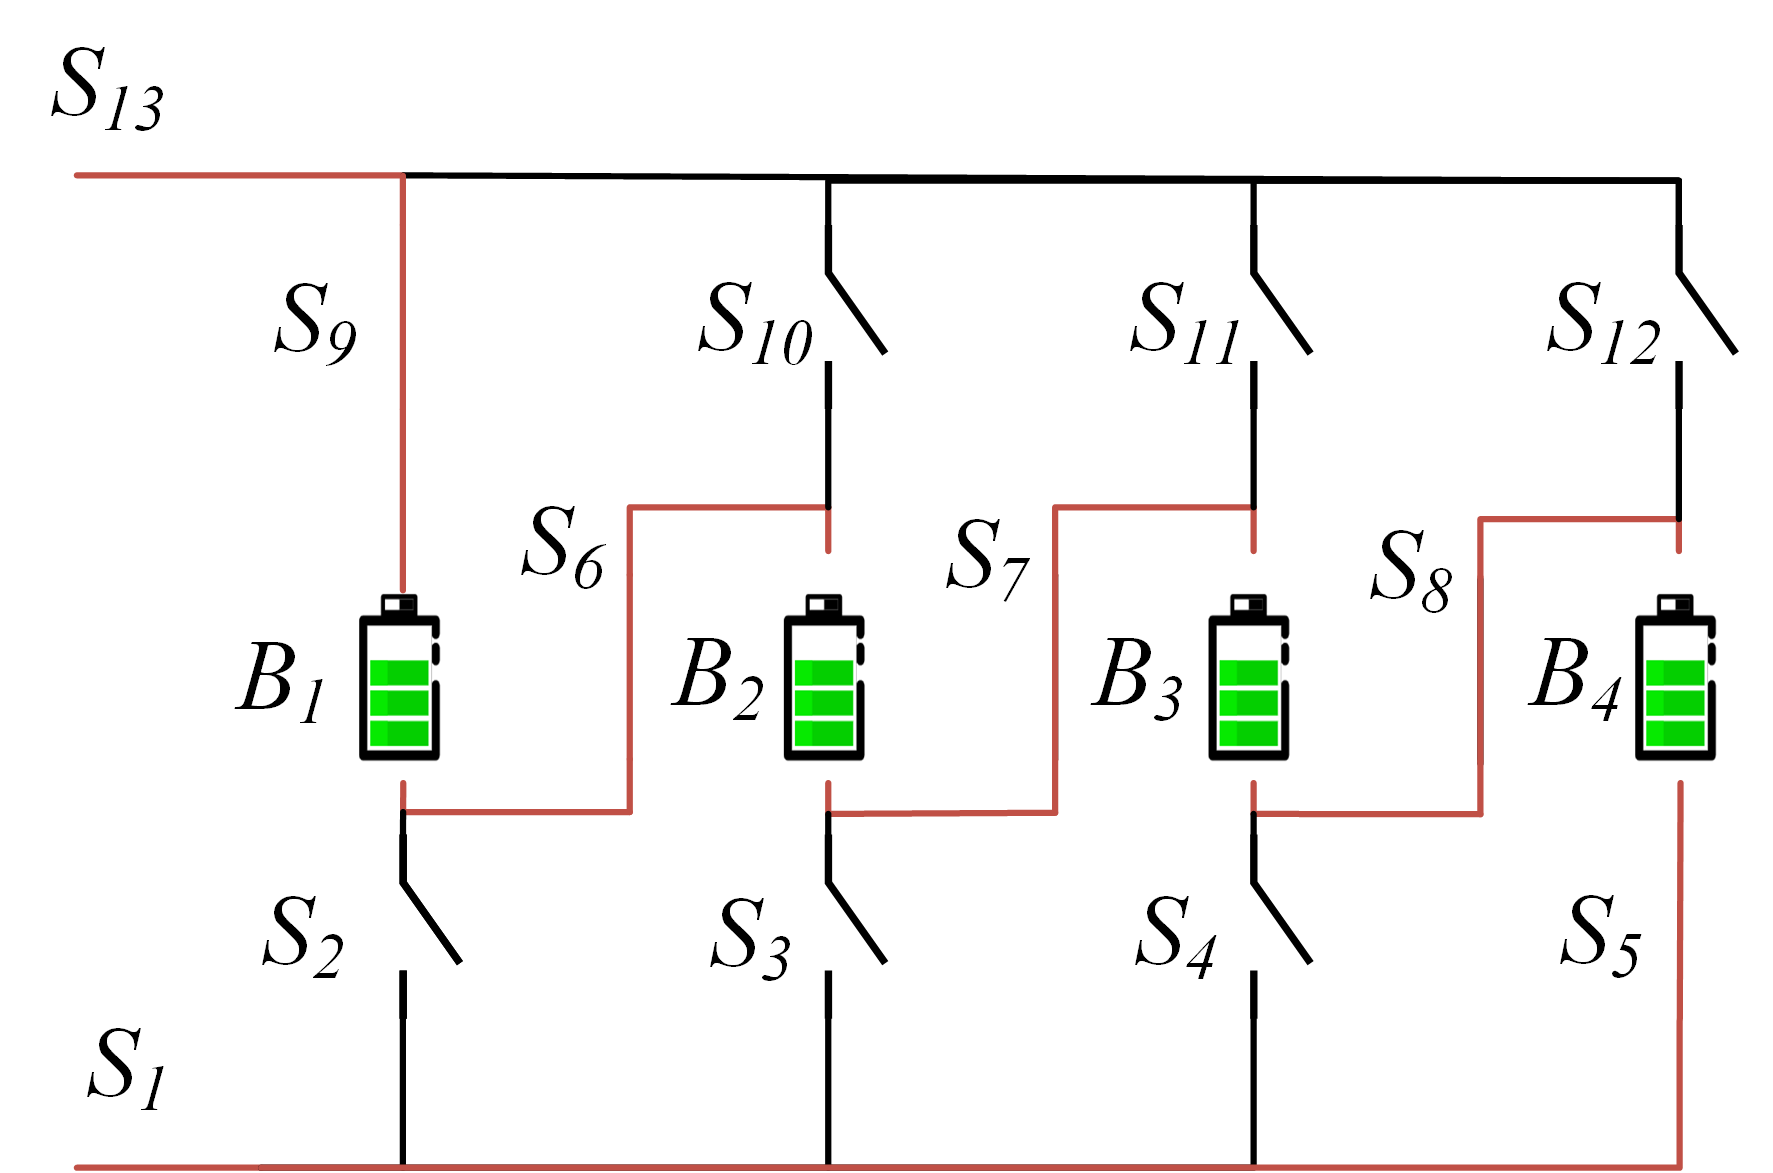
\includegraphics[width=\textwidth]{stru-V-serial.png}
        \caption{}
        \label{fig:stru-Visairo-serial}
    \end{subfigure}
    \\
    \begin{subfigure}[b]{0.45\textwidth}
        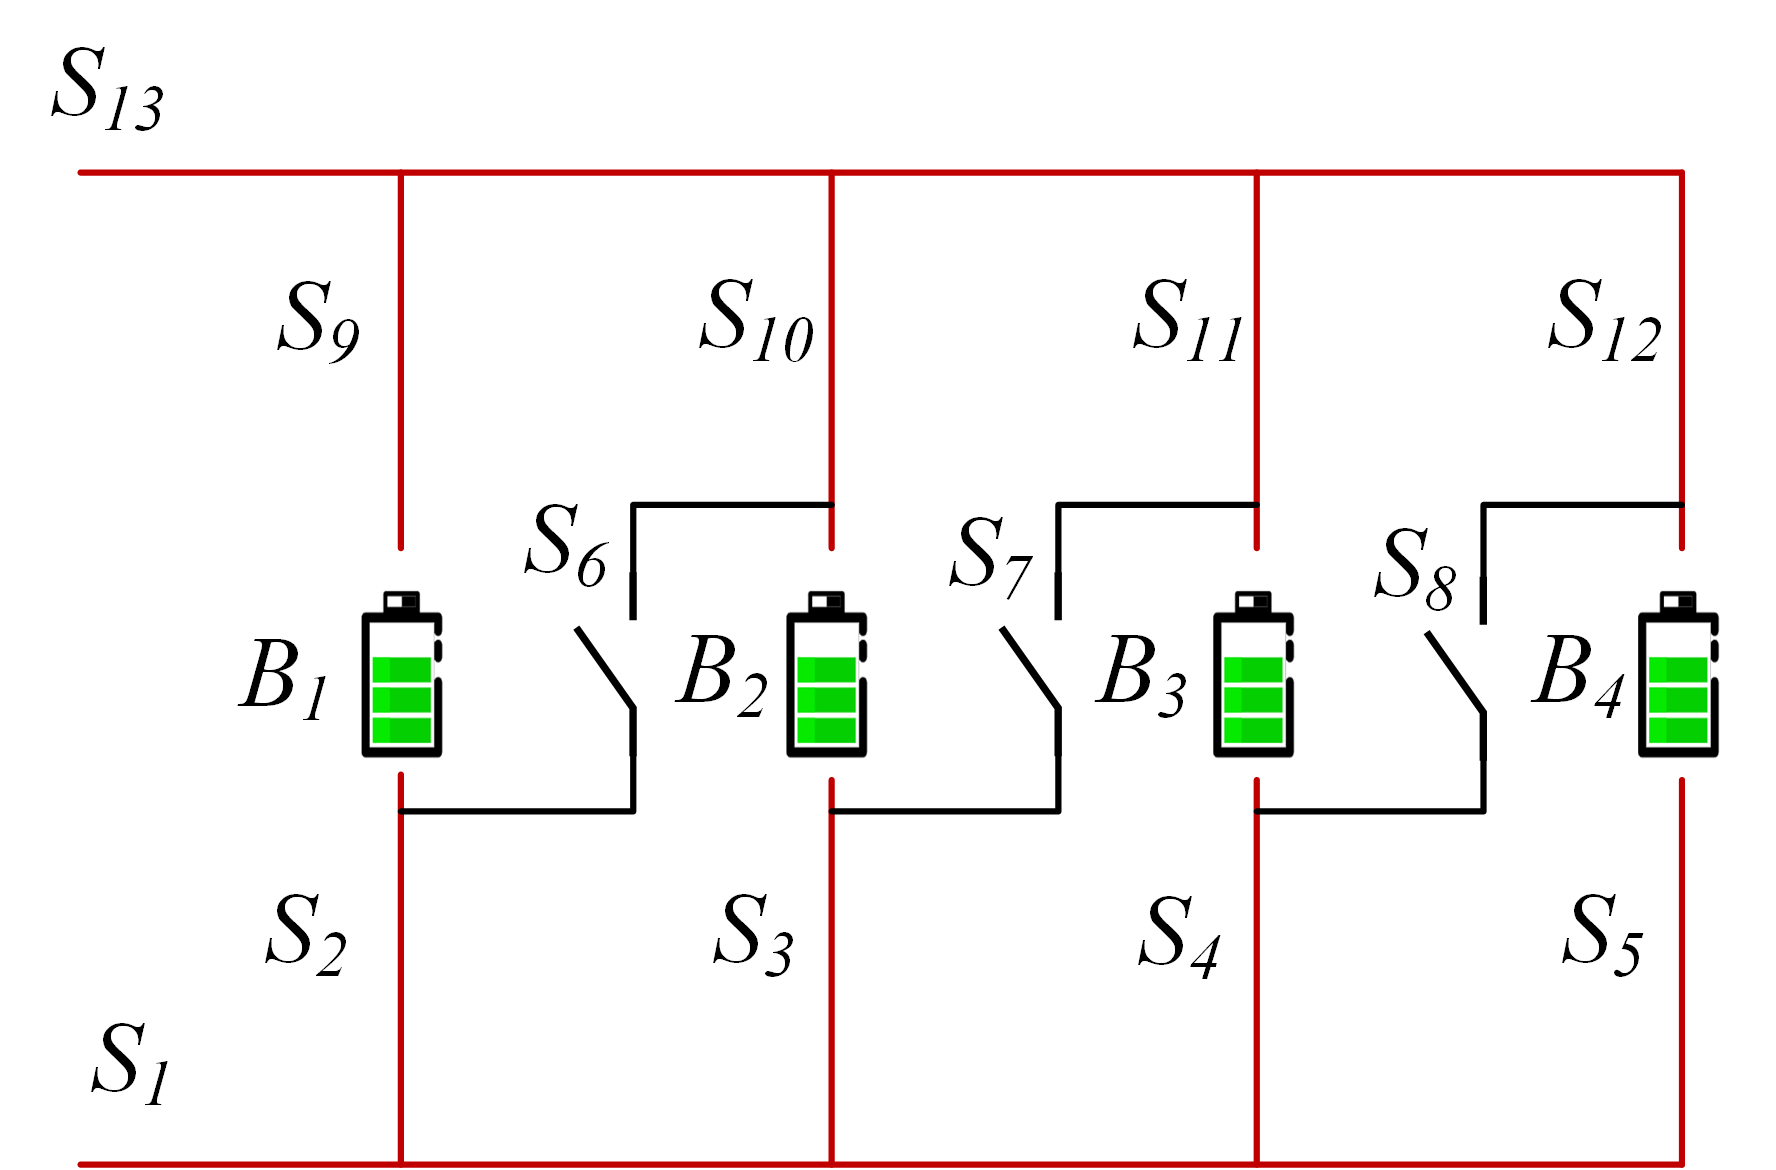
\includegraphics[width=\textwidth]{stru-V-parallel.png}
        \caption{}
        \label{fig:stru-Visairo-parallel}
    \end{subfigure}
    \hspace{0.05\textwidth}
    \begin{subfigure}[b]{0.45\textwidth}
        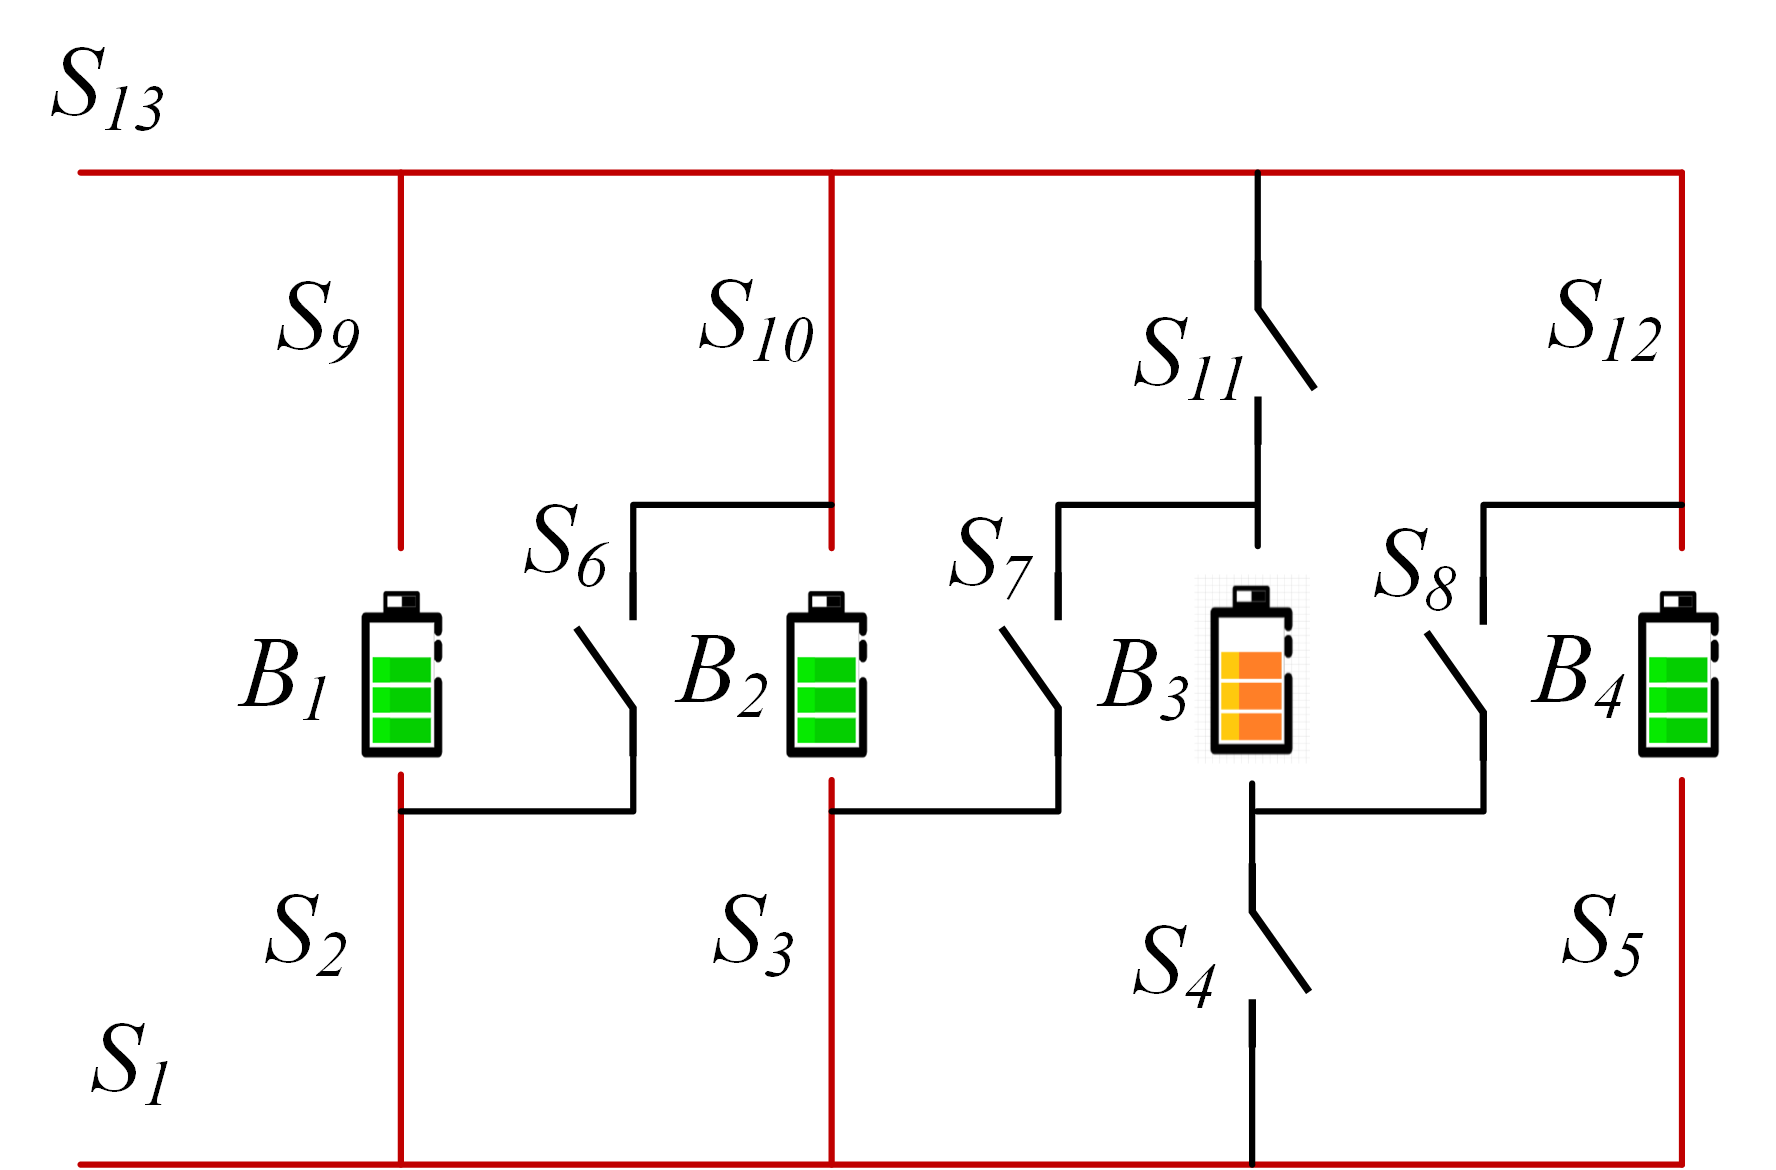
\includegraphics[width=\textwidth]{stru-V-isolate.png}
        \caption{}
        \label{fig:stru-Visairo-isolate}
    \end{subfigure}
    \caption{
        (a) The RBS structure proposed by Visairo\cite{visairoReconfigurableBatteryPack2008}, with
        all batteries in (b) series connection, (c) parallel connection, and
        (d) battery $B_3$ isolated.
        }
    \label{fig:arch}
\end{figure}

\added{
Recently, various types of RBS with different flexibility and reconfigurability have been designed to meet application requirements. 
For example, Ci et al. \cite{ci2007novel} proposed a RBS structure that can dynamically adjust the batteries discharge rate to fully exploit the available capacity of each battery. 
Jan's \cite{9209774,engelhardt2021double} structures had the ability to reconfigure structures with variant batteries in series to reach the voltage requirements during electric vehicle charging, which constantly change.
The structure proposed by Visairo et al.\cite{visairoReconfigurableBatteryPack2008}, as shown in Figure \ref{fig:stru-Visairo}, can change the system's output voltage based on load conditions, thereby reducing the power loss of the voltage regulator during the power supply process and improving energy utilization efficiency. 
For the same purpose to enhance the energy efficiency of the system, Lawson et al. \cite{lawsonSoftwareConfigurableBattery2012} and He et al. \cite{he2014reconfiguration} also proposed simplified structures which has less switches than Visairo's design.
Kim et al. \cite{kim2009dynamic} improved the system's ability to recover from battery failures by introducing multiple ports to the structure. 
The complex structure between batteries and switches enables the flexibility of RBS, but also brings the challenges in design and control of system. 
Thus, several approaches to analyze the RBS structure and performance have been proposed in the literature to tackle these challenges.
For instance, 
Han et al.\cite{han2021analysis} derived an analytical expression for the maximum switch current during battery system reconfiguration for a specific RBS structure. 
This helps guide the selection of switches and provide support for the hardware design of RBS.
Chen et al.\cite{chenSneakCircuitTheory2021} proposed a systematic approach based on the sneak circuit theory to fundamentally avoid the short-circuit problem of reconfigurable battery systems. 
They thoroughly analyzes all paths between the cathode and anode of each battery in the RBS and identifies paths that only contain switches as short-circuit paths for pre-checking before system reconfiguration. 
}


\added{
In spite of maximum switch current mentioned above, the maximum allowable current (MAC), defined as the maximum current allowed by system under the constraints of the battery cell, is another critical indictor of RBS that need to be evaluated during the design or control process of system. 
It helps the designers to assess whether the RBS meets the output current requirements, and contribute to the formulation of appropriate and safe management strategies for the battery management system (BMS).
Unfortunately, few studies on the RBS structure analysis have been conducted to determine the MAC of RBSs.
A intuitive and straightforward method is to enumerate all possible switch states and calculate the output current of the system under each reconfigurated structure.
But this method is inefficient and time-consuming, especially for RBSs with a large number of switches.
}


\deleted{
The complex connection structure between batteries and switches in the RBS provides flexibility but also introduces challenges in design and operational control. 
Unlike traditional BESSs with fixed outputs, the RBS output must be dynamically adjusted by controlling switch states to meet external load requirements. 
This necessitates additional, time-consuming output performance analysis during design and corresponding control strategies. 
An incorrect switch control strategy may cause battery short-circuiting or overload, risking the entire system. 
The Maximum Allowable Current (MAC), an RBS performance indicator, can guide designers in addressing this issue. 
MAC is defined as the maximum RBS output current that ensures each battery's current remains within a safe range.
Therefore, it provides a benchmark for RBS output current, protecting individual batteries and identifying overall system output limits during operation. 
Despite its importance, no method currently exists for automatically evaluating MAC for RBSs.
In particular, when one or more random cells are isolated, there is still no method to determine the MAC of the remaining RBS in time to assist the system in adjusting the control strategy timely. 
A universal and automatical method for calculating RBS MAC is urgently needed for practical applications.
}


\added{
To solve this issue, a new method to effectively evaluate the MAC of RBS is proposed in this paper. 
First, a greedy algorithm is designed to search the possible circuit topology of RBS with MAC effciently.
Meanwhile, an improved direct graph model, considering the voltage, internal resistance, and maximum allowable current of the battery, and the external load, is porposed to obtain the accurate current value of RBS under specific circuit topology. 
To the best of our knowledge, the present work is the first to develop an efficient calculation method of RBS MAC.
}
\deleted{In this study, a directed graph model and greedy algorithm are employed to determine the MAC of RBS and the corresponding control strategy, effectively calculating the MAC for RBSs with arbitrary structures, including scenarios with isolated batteries.}
\added{The main contributions of the paper can be summarized as follows:}
\begin{itemize}
  \item \added{Proposing a effective method to determine the MAC of RBSs with arbitrary structures, including scenarios with isolated batteries.}
  \item \added{Application of the greedy algorithm to solve the MAC problem, whose computational complexity is greatly reduced compared with the brute force algorithm.}
  \item \added{introducing an improved directed graph model, considering the voltage, internal resistance, and maximum allowable current of the battery, and the external load, to achieve the current analysis of the RBS.}
\end{itemize}


The remainder of this paper is organized as follows: 
Section II presents the framework and details of the proposed directed graph model and the greedy algorithm. 
Section III demonstrated a case study of using the proposed method to determine the MAC of a novel and complex structure. 
The calculation results \added{, the algorithm's computational complexity} and scenarios such as batteries isolation also are discussed. 
Finally, the concluding remarks are drawn in Section IV.

\section{Methodology}

The central principle of this method is to make the batteries in RBS connected in parallel as much as possible, thereby maximizing the output current of the RBS.
To universally and automatically achieve this, the overall process is divided into four steps, as shown in Figure \ref{fig:main}.
Firstly, a directed graph model is established for subsequent \replaced{computations.}{computing,} \replaced{The model}{, which} not only contains the connected relationships between batteries and switches, but also retains the performance parameters of the batteries.
Subsequently, based on the equivalent circuit, the MAC problem is transformed into specific objective functions and constraints.
Then, the shortest paths (\replaced{$SP$}{SP}s, where additional batteries and switches on the path are penalized as distance) for the batteries are obtained using the Dijkstra algorithm to guide the batteries in the RBS connect in parallel.
Finally, a greedy algorithm is employed to organize the switches, allowing the batteries to connect via their \replaced{$SP$}{SP}s while satisfying the constraints, resulting in the MAC of the RBS.

\begin{figure}[htbp]
    \centering
    \begin{subfigure}[b]{0.8\textwidth}
        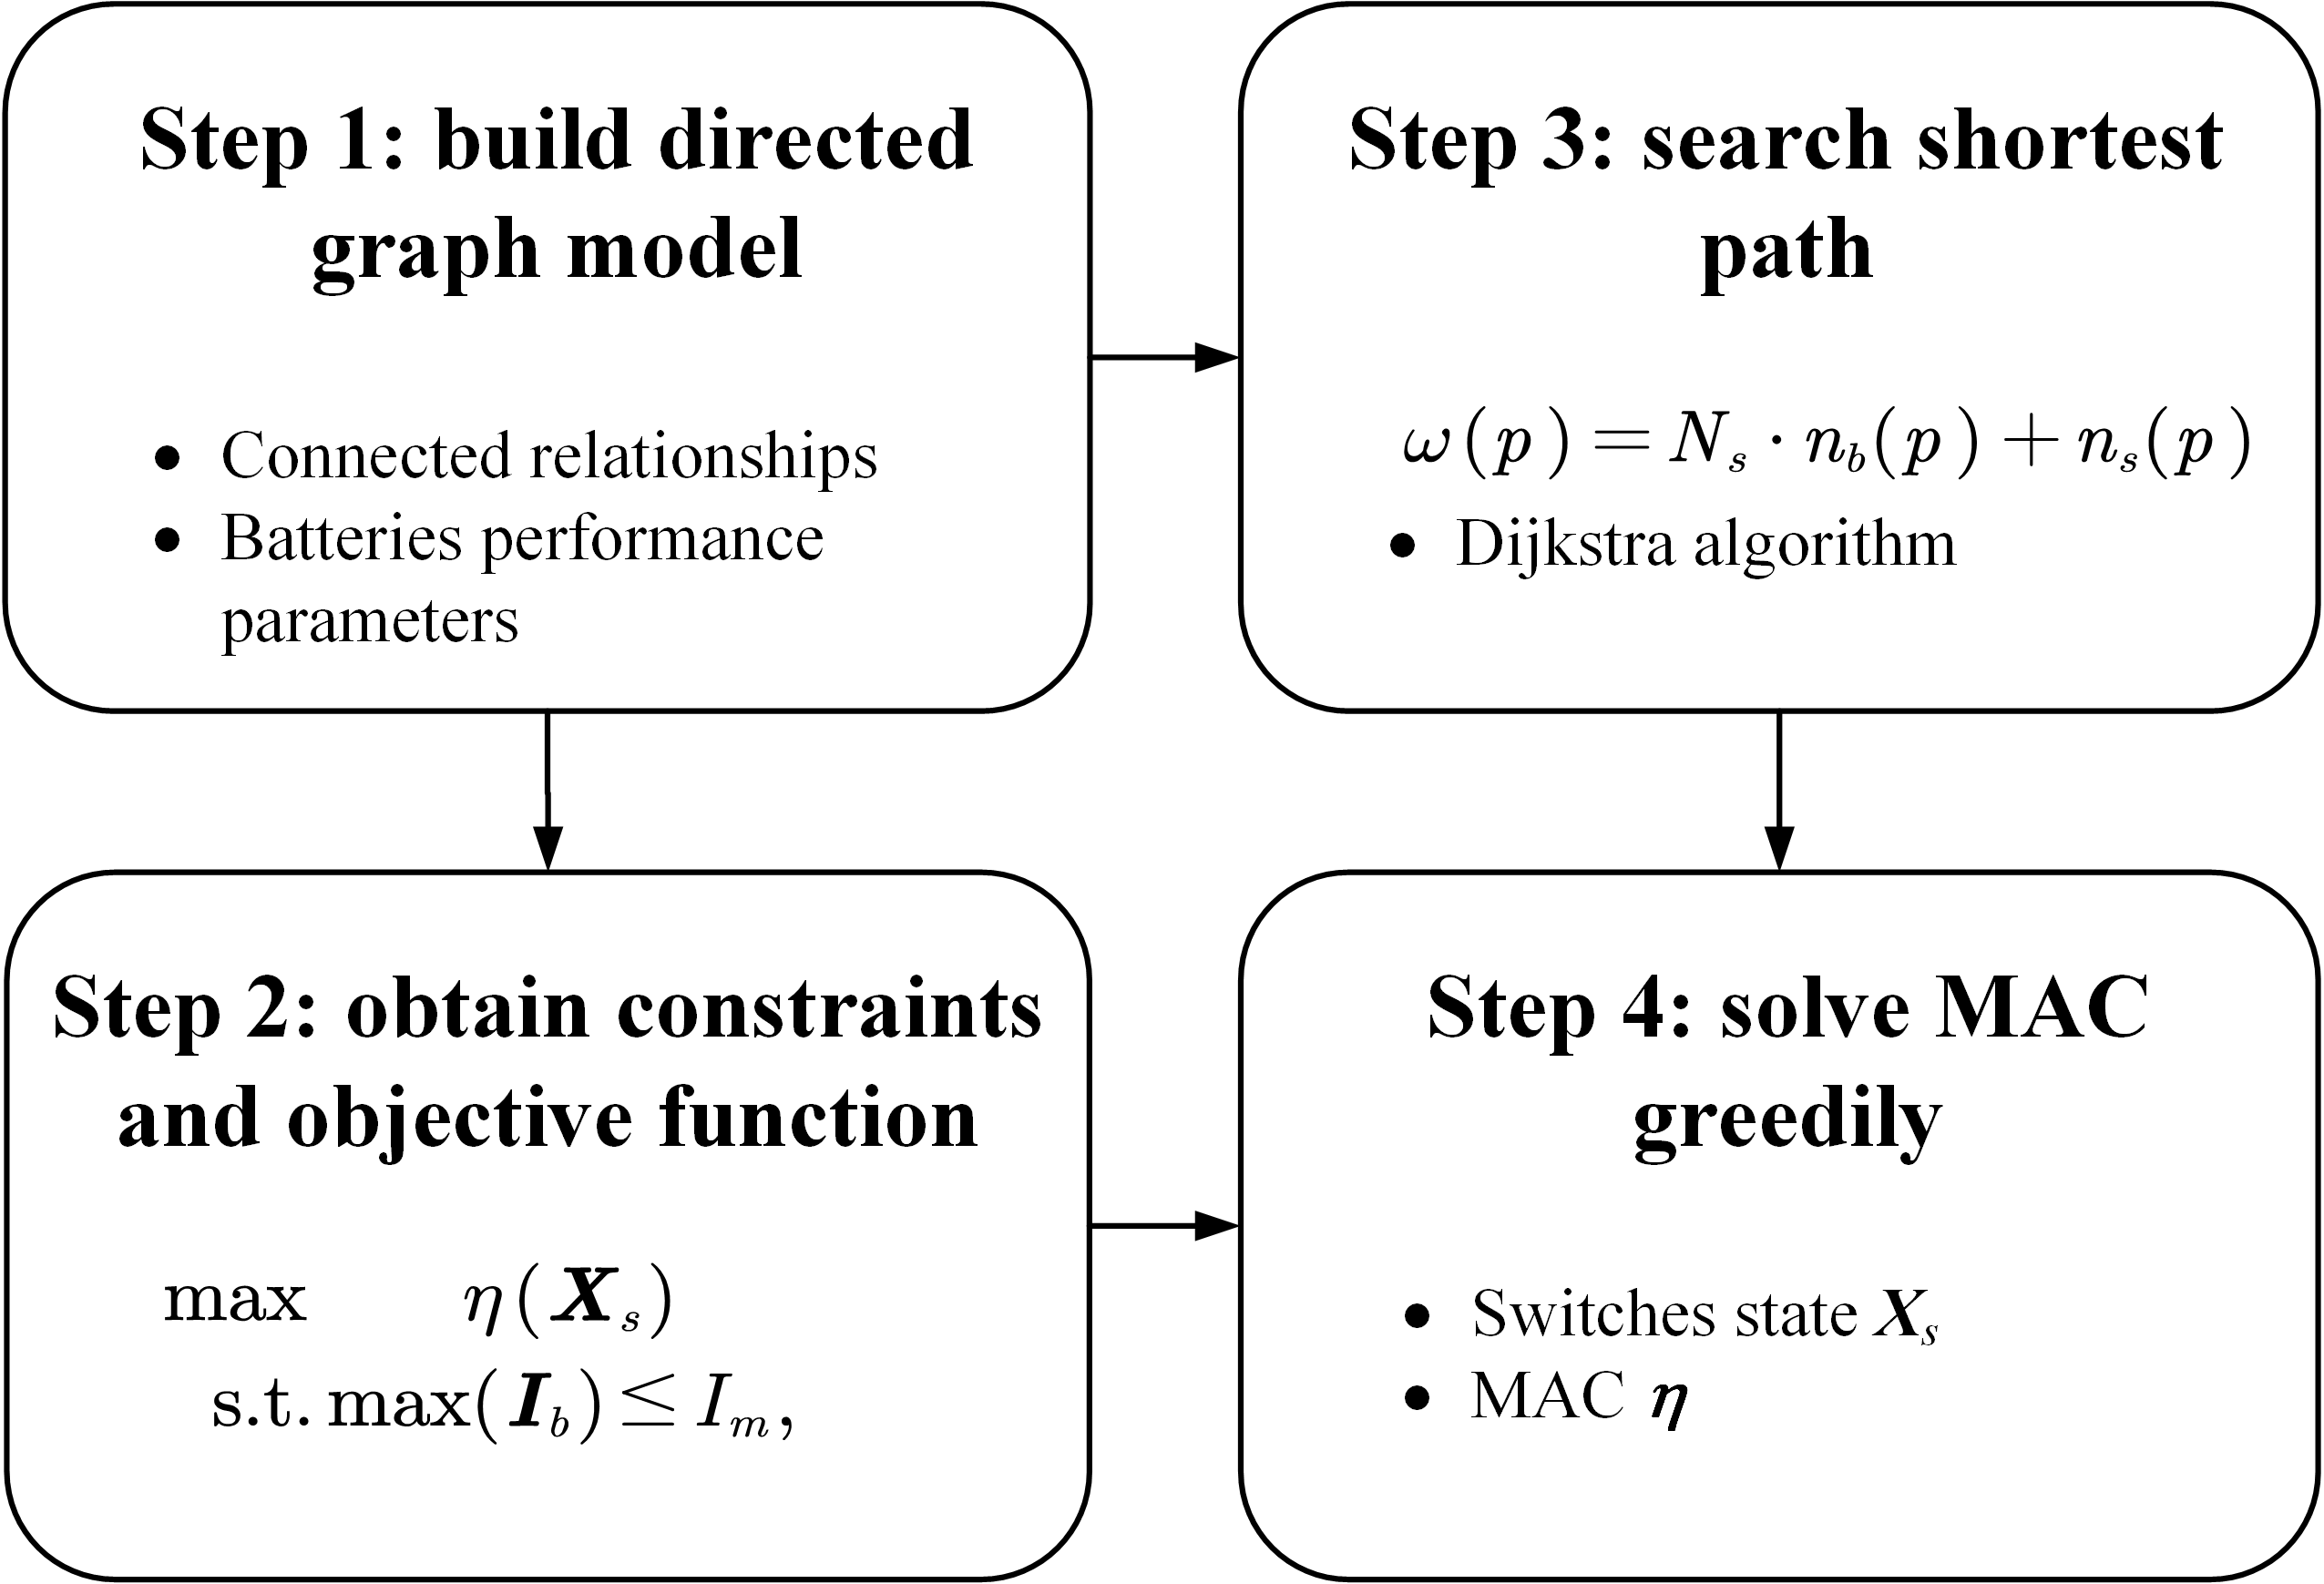
\includegraphics[width=\textwidth]{main.png}
    \end{subfigure}
    \caption{ 
        Diagram of this method, which contains four main steps.
    }
    \label{fig:main}
\end{figure}

\subsection{Directed graph Model}

\begin{figure}[htbp]
    \centering
    \begin{subfigure}[b]{0.31\textwidth}
        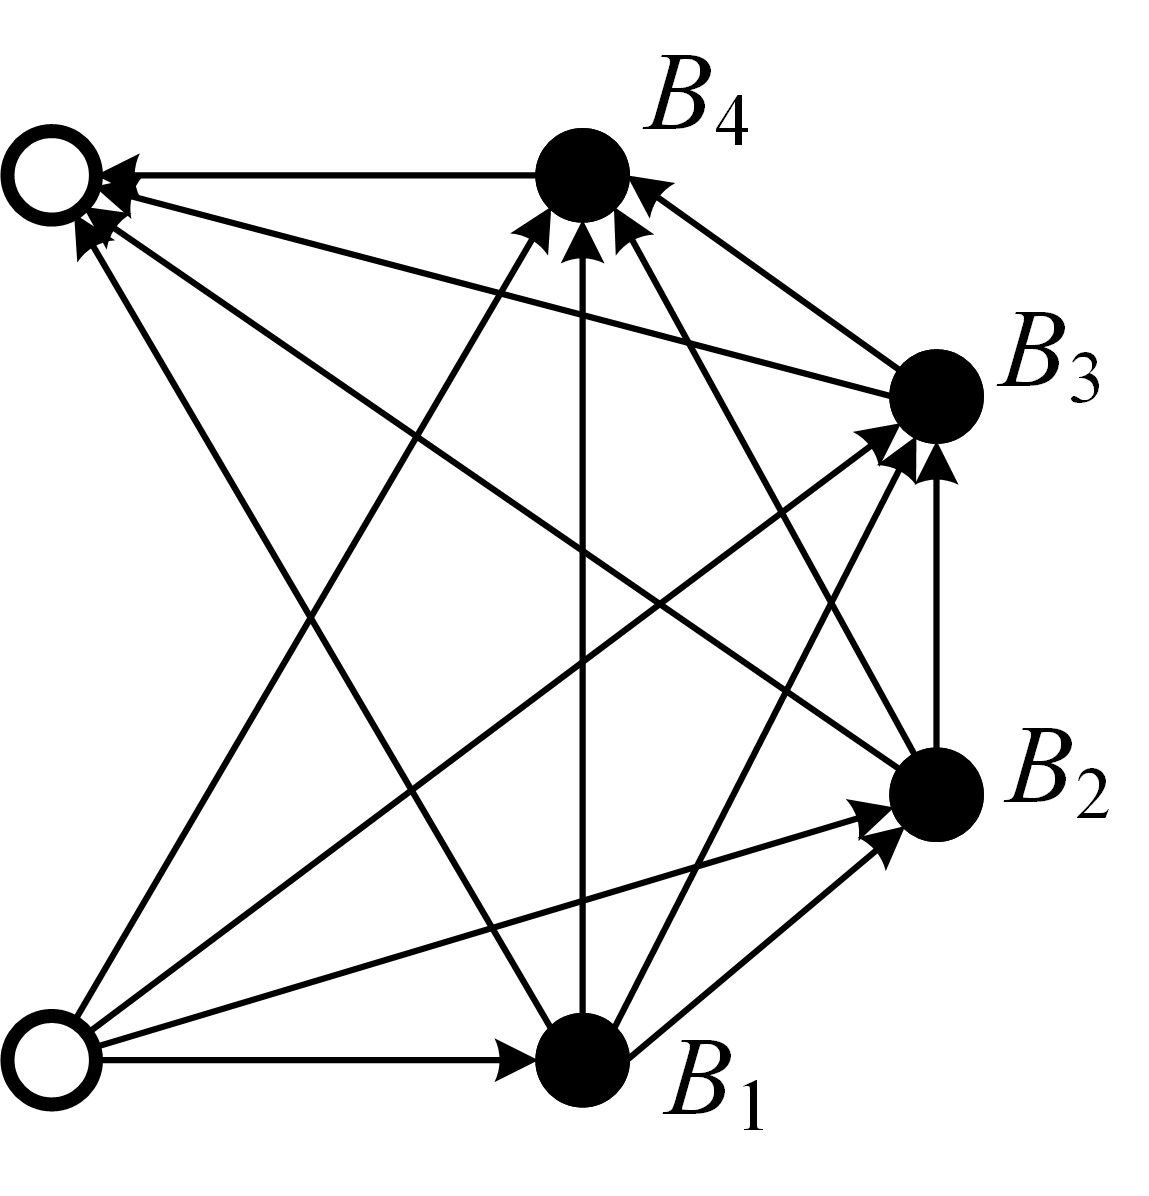
\includegraphics[width=\textwidth]{direct-graph-he.png}
        \caption{}
        \label{fig:direct-graph-he}
    \end{subfigure}
    \hspace{0.02\textwidth}
    \begin{subfigure}[b]{0.23\textwidth}
        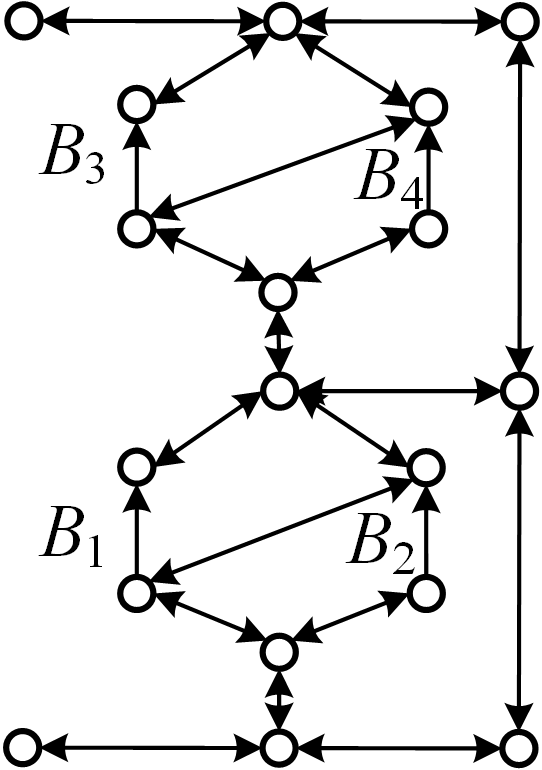
\includegraphics[width=\textwidth]{direct-graph-xu.png}
        \caption{}
        \label{fig:direct-graph-xu}
    \end{subfigure}
    \hspace{0.02\textwidth}
    \begin{subfigure}[b]{0.24\textwidth}
        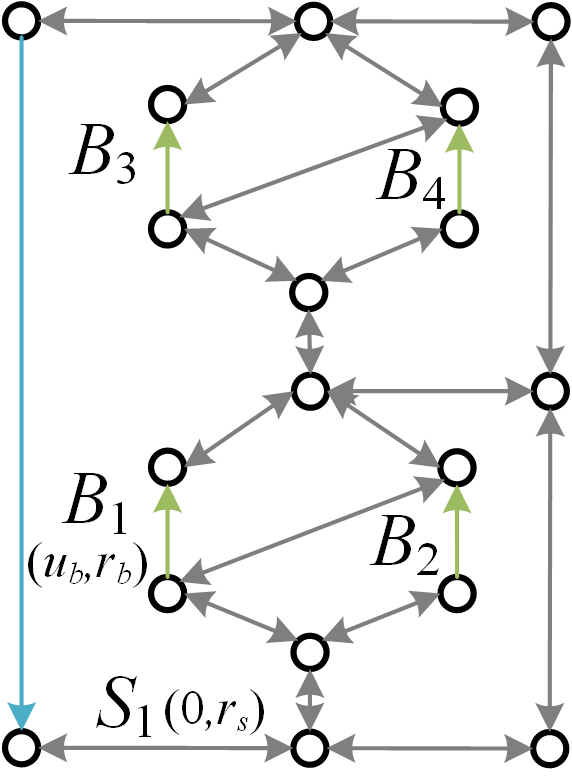
\includegraphics[width=\textwidth]{direct-graph-my.png}
        \caption{}
        \label{fig:direct-graph-my}
    \end{subfigure}
    \\
    \begin{subfigure}[b]{0.8\textwidth}
        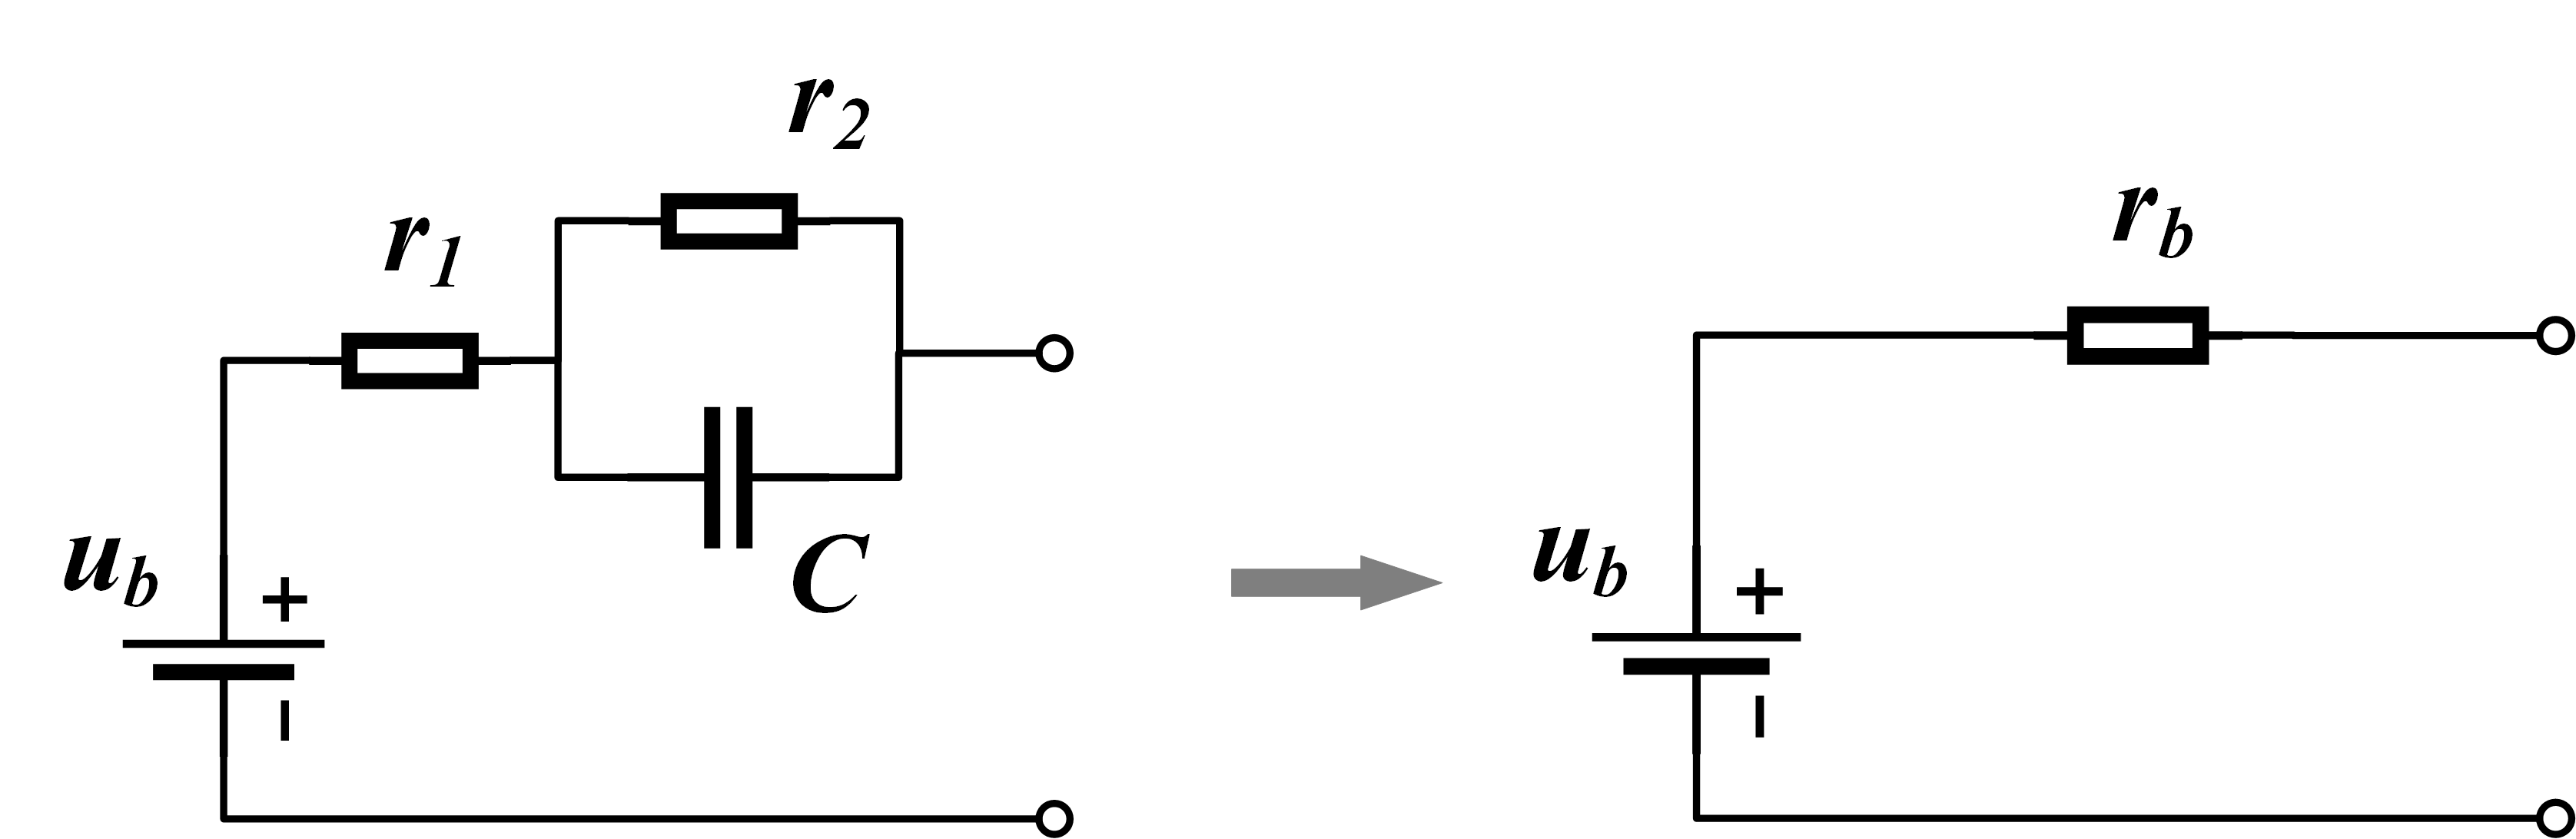
\includegraphics[width=\textwidth]{battery_simple.png}
        \caption{}
        \label{fig:battery_simple}
    \end{subfigure}
    \caption{ 
        Directed graph models used in (a) He's work \cite{heExploringAdaptiveReconfiguration2013}, (b) our previous work , and (c) \added{the improved model in} this paper.
        (d) The equivalent circuit of a battery in this method.
    }
\end{figure}

He et al. \cite{heExploringAdaptiveReconfiguration2013} once proposed an abstracted directed graph model for RBS, where the nodes represented the batteries, the edges represented the configuration flexibility, and the weight of each vertex corresponded to the battery voltage ( Figure \ref{fig:direct-graph-he}). 
The model effectively captured all potential system configurations and offered a direct metric for configuration flexibility, but it did not specify the physical implementation of the connectivity between batteries, meaning one graph might \replaced{correspond to}{have had} multiple RBS structures.
We previously proposed a novel directed graph model that, \replaced{completely different from}{in contrast to} He's model, used nodes to represent the connections between batteries and switches, and directed edges to represent batteries and switches (Figure \ref{fig:direct-graph-xu}), allowing for a one-to-one correspondence between the RBS structure and the directed graph model. 
This model was able to accurately and comprehensively represent the RBS topological structure but could not be used for quantitative MAC calculations due to the lack of consideration \replaced{on}{for} \replaced{the voltage, internal resistance and maximum allowable current of the battery}{battery and switch performance parameters}. 
To address this, an \replaced{improvement on our previous model is conducted by}{improved directed graph model is used here based on our original model,} adding electromotive force and resistance attributes on the edges based \replaced{on its}{to} equivalent circuits \deleted{(Figure \ref{fig:direct-graph-my})}.
The model also considers the external load as an equivalent resistance and integrate it into the analysis, making it a complete circuit model for later circuit analysis.
\added{Figure \ref{fig:direct-graph-my} shows the improved directed graph model used in this paper.}
The following will provide a detailed explanation of the method for equating the components in RBS and constructing the directed graph model.


In order to use circuit analysis methods to solve the MAC of the RBS, the components in the RBS are equated to ideal circuit elements.
\added{For instance,} \replaced{a}{A}s shown in Figure \ref{fig:battery_simple}, the battery in the RBS can be represented as a black-box circuit consisting of two resistors (i.e., $r_1$ and $r_2$) and a capacitor (i.e., $C$), known as the Thevenin model\cite{hongwenheStateofChargeEstimationLithiumIon2011,mousavig.VariousBatteryModels2014}.
With an emphasis on the stable output of the RBS, the capacitor in the Thevenin model can be considered as an open circuit without affecting the steady-state current.
Therefore, the battery $i$ in the RBS can be simplified as the series connection between a constant voltage source $u_{i}$ and a resistor $r_{i}$.
Furthermore, the state of switch $j$ in the RBS is represented by a binary variable $x_j$, where 0 is for ON and 1 is for OFF, respectively.
When the switch is closed, it can be regarded as a resistor with a very small resistance value $r_{j}$.
Lastly, the external load is considered as a resistor with a value of $R_o$.


For a given RBS structure, \replaced{its directed graph model $G(V,E)$ is constructed as follows:}{the directed graph model for the RBS is constructed as a directed graph $G(V,E)$ in such a way that:}
\begin{enumerate}
    \item Nodes:
        The nodes in the directed graph correspond to the connection points of components in the actual RBS. 
        Assuming there are a total of $N$ nodes in the RBS, for the sake of convenience, the anode of the RBS is denoted as $v_1$ and the cathode as $v_N$.
    \item Edges:
        The edges in the directed graph correspond to the batteries, switches, and external electrical loads in the actual RBS.
        Therefore, there are three types of directed edges. 
        For a battery $B_i$, its directed edge $e_i$ is drawn from the cathode to the anode, as the battery only allows current to flow in one direction when in operation.
        For a switch $S_j$, since it is allowed to work under bi-directional currents, it is represented by a pair of directed edges with two-way directions. 
        Regarding the external electronic load, as it is connected to the anode and cathode of the RBS, a directed edge from $v_N$ to $v_1$ is used to represent it. 
        In conclusion, for a given RBS structure with $N_b$ batteries and $N_s$ switches, the total number of directed edges is $N_b+2N_s+1$, where 1 refers to the external electrical load.
    \item Edges' attributes:
        Each edge is assigned two attributes, voltage difference and resistance, based on the equivalent method mentioned above.
        The values for the battery $B_i$, switch $S_j$, and external loads correspond to $(u_i, r_i)$, $(0, r_j)$, and $(0, R_o)$, respectively.
\end{enumerate}

\subsection{Constraints and Objective Function}

\replaced{For a given RBS, determination of its MAC}{Based on the definition of MAC, determining the MAC of RBS} involves maximizing the RBS output current while ensuring that the currents of all batteries do not exceed the batteries' maximum allowable current. 
In this subsection, the constraints and objective function to solve the RBS's MAC will be established through circuit analysis, based on \replaced{its directed graph model provided in the previous subsection}{the previously constructed directed graph model}.


First, the topology in the directed graph model is represented in matrix form $\bm{A}$, known as the incidence matrix , \replaced{defined}{to facilitate circuit analysis.
The specific definition of the incidence matrix is shown} in Equation \ref{eq:A}.
\begin{align}\label{eq:A}
    a_{kl}=
    \begin{cases}
        1,  & \text{edge $l$ leaves node $k$},\\
        -1, & \text{edge $l$ enters node $k$},\\
        0,  & \text{otherwise}.
    \end{cases}
\end{align}
For a directed graph consisting of $N$ nodes and $N_b+2N_s+1$ directed edges, its incidence matrix $\bm{A}$ is an $N\times(N_b+2N_s+1)$ matrix. 
In this matrix, the rows and columns represent the nodes and edges of the directed graph, respectively.
By distinguishing the components in the RBS corresponding to each column , $\bm{A}$ can be rewritten as:
\begin{equation}\label{eq:A_bso}
    \bm{A} =
    \begin{bmatrix}
        \bm{A}_b & \bm{A}_s & \bm{A}_o
    \end{bmatrix},
\end{equation}
where $\bm{A}_b$, $\bm{A}_s$ and $\bm{A}_o$ are the sub-matrices corresponding to the batteries, switches and external electrical load, respectively.
To alleviate computational complexity, matrix $\bm{A}$ undergoes dimensionality reduction.
Since each directed edge has one node to leave and one to enter, the sum of the values in every column of $\bm{A}$ is zero.
Therefore removing \replaced{the last}{any single one} row will not result in a loss of information. 
\deleted{Without loss of generality, the last row is removed here.}
On the other hand, since each switch in the RBS is represented by a pair of directed edges with two-way directions, the two columns corresponding to the switch are mutually opposite.
Thus, for the sub-matrix $\bm{A}_s$, only one column is retained for each pair of columns representing the same switch.
As a result, $\bm{A}$ can be reduced to a $(N-1)\times(N_b+N_s+1)$ matrix, denoted as $\bm{\tilde{A}}$, for further calculation of current and voltage.
Similar to Equation \ref{eq:A_bso}, $\bm{\tilde{A}}$ can be rewritten as:
\begin{equation}\label{eq:A_bso_tilde}
    \bm{\tilde{A}} =
    \begin{bmatrix}
        \bm{\tilde{A}}_b & \bm{\tilde{A}}_s & \bm{\tilde{A}}_o
    \end{bmatrix}.
\end{equation}


After obtaining the incidence matrix, the currents of all batteries and output in RBS are determined by solving the circuit equations.
According to Kirchhoffs law, we have
\begin{align}\label{eq:Kirchhoffs_law}
    \begin{cases}
        \bm{\tilde{A}} \bm{I} = \bm{0}, \\
        \bm{U}        = \bm{\tilde{A}}^\T \bm{U}_n,
    \end{cases}
\end{align}
where $\bm{I}$ and $\bm{U}$ indicate the current and voltage difference arrays of the $N_b+N_s+1$ edges, respectively;
$\bm{U}_n$ is the voltage array of the $N-1$ nodes.
These directed edges are treated as generalized branches and expressed in matrix form as follows
\begin{equation}\label{eq:generalized_branches}
    \bm{I} = \bm{Y}\bm{X} \bm{U} - \bm{Y}\bm{X} \bm{U}_s +\bm{I}_s,
\end{equation}
where $\bm{U}_s$ and $\bm{I}_s$ denote the source voltage and source current of the generalized branches, respectively.
Because all batteries have been equivalent to voltage sources rather than current sources in the previous subsection, all elements of the array $\bm{I}_s$ are 0, 
while the elements of the array $\bm{U}_s$ are equal to the first attribute of the corresponding edges in the directed graph.
The $\bm{Y}$ in \added{Equation} \ref{eq:generalized_branches} is the admittance matrix of the circuit, defined as the inverse of the impedance matrix.
\replaced{The}{That is the} elements \replaced{on}{of} the diagonal \added{of} matrix $\bm{Y}$ are equal to the reciprocal of \added{the resistance, which is} the second attribute of the corresponding edges in the directed graph, and the off-diagonal elements \added{$\bm{Y}$} are 0.
The $\bm{X}$ is the state matrix, which describes whether the RBS batteries and switches are allowed to pass current.
It is defined as
\begin{equation}\label{eq:X}
    \bm{X} = \diag(
    \underbrace{1, 0 \cdots, 1}_{N_b~\text{of}~0/1},
    \underbrace{1, 0 \cdots, 1}_{N_s~\text{of}~0/1},
    1)
    =\begin{bmatrix}
        \bm{X}_b & & \\
        & \bm{X}_s &\\
        & & 1
    \end{bmatrix}.
\end{equation}
Where the elements $x_i$ of the matrix $\bm{X}_b$ represent whether the battery $i$ has been removed from the circuit, with $x_i=1$ indicating removal and $x_i=0$ indicating that it is still available to supply power. 
When all batteries are health and capable of providing current to the external load, $\bm{X}_b$ is an identity matrix. 
The elements $x_j$ of the matrix $\bm{X}_s$ represent whether the switch $j$ is closed, with $x_j=1$ indicating closure and $x_j=0$ indicating disconnection, which is consistent with the previous subsection.


Theoretically, the output current $I_o$ and the currents of each battery $\bm{I}_b$ in the RBS  can be determined by solving Equations \ref{eq:Kirchhoffs_law}, \ref{eq:generalized_branches}, and \ref{eq:X} under any given state $\bm{X}$.
In order to obtain specific constraint conditions and objective functions, it is further assumed that all batteries have the same electromotive force and internal resistance, denoted as $u_b$ and $r_b$, respectively.
This allows for the derivation of explicit expressions for $I_o$ and $\bm{I}_b$.
After derivation and simplification, the output current $I_o$ and the currents of each battery $\bm{I}_b$ are ultimately represented as Equations \ref{eq:I_o} and \ref{eq:I_b}, respectively.
\begin{equation}\label{eq:I_o}
    I_o = \frac{1}{R_o r_b} \bm{\tilde{A}}_o^\T \bm{Y}_n^{-1}(\bm{X}) \bm{\tilde{A}}_b \bm{U}_b,
\end{equation}
\begin{equation}\label{eq:I_b}
    \bm{I}_b = \frac{1}{r_b^2}[\bm{\tilde{A}}_b^\T \bm{Y}_n^{-1}(\bm{X}) \bm{\tilde{A}}_b\bm{U}_b -r_b \bm{U}_b],
\end{equation}
where $\bm{U}_b$ is a $N_b\times 1$ array with all elements equaling to $u_b$;
$\bm{Y}_n$ is the equivalent admittance matrix of the circuit, defined as
\begin{equation}\label{eq:Yn}
    \bm{Y}_n (\bm{X}) = \frac{1}{R_o} \bm{\tilde{A}}_o\bm{\tilde{A}}_o^\T + \frac{1}{r_b} \bm{\tilde{A}}_b\bm{X}_b\bm{\tilde{A}}_b^\T + \frac{1}{r_s}\bm{\tilde{A}}_s\bm{X}_s\bm{\tilde{A}}_s^\T.
\end{equation}


To characterize the current output capacity of the RBS structure under different switching states, an indicator $\eta$ is defined by the ratio of $I_o$ and $\max (\bm{I}_b)$ shown in Equation \ref{eq:eta}:
\begin{equation}\label{eq:eta}
    \eta = \frac{I_o}{\max (\bm{I}_b)}.
\end{equation}
Finally the problem of solving MAC can be formulated as
\begin{align}
    & \max \eta(\bm{X}_s) \label{eq:max_eta}\\
    \text{s.t.} & \max (\bm{I}_b) \leq I_m, \label{eq:Ib_leq_Im}
\end{align}
where $I_m$ is the maximum allowable current of the battery.


However, it is \added{still} computationally difficult to solve \ref{eq:max_eta} because of the $\bm{Y}_n^{-1}$.
On one hand, due to the introduction of nonlinear terms by $\bm{Y}_n^{-1}$, many effective methods in linear optimization are not suitable for this \replaced{scenario}{problem}.
On the other hand, the rank of $Y_{n}$ is proportional to the number of batteries and switches, which can be very large for a large RBS system, leading to significant computational burden.
Therefore, intelligent algorithms that rely on evolving by iteration may face efficiency \replaced{problem}{issues} when dealing with large RBS system.
In order to address this issue, the problem should be considered from the perspective of guiding the RBS to reconstruct as many parallel structures as possible.
Consequently, a greedy algorithm based on the shortest path is proposed. 
The detailed implementation process is presented in the following two subsections.

\subsection{Shortest Path}

The path $p$ used in this method is defined as the complete route that passes through one battery (or a consecutive series of batteries) and closed switches, connecting the anode $v_1$ to the cathode $v_N$ of the RBS.
By applying a penalty to the series-connected batteries on the path, where additional batteries imply a longer distance, the algorithm encourages the RBS to form parallel structures as much as possible.
Meanwhile, to reduce the number of switches controlled during the reconstruction process, a penalty is also applied to the total number of switches on the path, while ensuring the minimum number of batteries.
Therefore, the distance $\omega$ of the path $p$ is defined by the following equation: 
\begin{equation}\label{eq:weight}
    \omega(p) = N_s \cdot n_b (p) + n_s (p),
\end{equation}
where $N_s$ is the total number of switches in the system; 
$n_b(p)$ and $n_s(p)$ are number of batteries and switches in the path $p$ respectively. 
Moreover, the shortest path $SP_i$ is defined as the path with the minimum $\omega$ for battery $i$, as shown in the following equation:
\begin{equation}\label{eq:def_sp}
    SP_i = \mathop{\arg\min}_{p \in P_i} \omega(p),
\end{equation}
where $P_i$ is the set of all paths from $v_1$ to $v_N$ which pass through the directed edge $i$.


The $SP_i$ can be solved by the Dijkstra algorithm.
The Dijkstra algorithm is a graph search method that finds the shortest path between two given nodes in a weighted graph, efficiently solving the single-source shortest path problem.
Assuming that the cathode and anode of battery $i$ are denoted as $v_i^-$ and $v_i^+$ respectively, the path $p$ of battery $i$  can be divided into three segments : $v_1 \rightarrow v_i^-$, $v_i^+ \rightarrow v_N$, and $v_i^- \rightarrow v_i^+$.
The $v_i^- \rightarrow v_i^+$ is the directed edge corresponding to battery $i$. 
With the Dijkstra algorithm, shortest paths for the $v_1 \rightarrow v_i^-$ and $v_i^+ \rightarrow v_N$ can be calculated under the weights given in Equation \ref{eq:weight}, denoted as $SP(v_i^- \rightarrow v_i^+)$ and $SP(v_i^+ \rightarrow v_N)$, respectively.
Finally, the $SP_i$ for battery $i$ is formed by the complete path with $SP(v_1 \rightarrow v_i^-)$, $v_i^- \rightarrow v_i^+$, and $SP(v_i^+ \rightarrow v_N)$.

\subsection{Greedy Algorithm}\label{subsec:greedy_solution}

From the perspective of series/parallel connections, integrating more batteries into the circuit through their shortest paths ($SP$s) results in a larger number of batteries connected in parallel, thereby increasing the total output current of the RBS.
However, conflicts may arise between the $SP$s of different batteries. 
For instance, the $SP$s of two batteries might form a short-circuited RBS structure, which is not allowed. 
To address this issue, a greedy algorithm is employed to incorporate as many $SP$s as possible while satisfying the reconstruction requirements.

The algorithm, as illustrated in Figure \ref{fig:flowchart}, can be summarized as follows, with the corresponding pseudo-code presented in Algorithm 1. % \ref{alg:greedy}.
First, the shortest paths ($SP$s) are obtained using Equations \ref{eq:weight} and \ref{eq:def_sp} in conjunction with Dijkstra Search. 
Next, the matrix $\bm{A}$ is calculated using Equation \ref{eq:A}, and the initial $N_{set}$ is set to $N_b$. 
The algorithm iteratively checks different combinations of $c_b$ batteries from $N_b$ and updates $N_{set}$ using a dichotomy method until convergence is reached. 
For each combination, the algorithm constructs an effective solution if possible, and calculates the currents $I_o$ and $\bm{I}_b$ using Equations \ref{eq:I_o} and \ref{eq:I_b}. 
If the maximum current $\bm{I}_b$ is less than or equal to $I_m$, the $\eta$ is calculated using Equation \ref{eq:eta}, and the maximum $\eta$ is updated accordingly. 
Finally, the algorithm outputs the maximum $\eta$ once $N_{set}$ converges.

% \tikzset{
%   meta box/.style={draw, black, very thick, text centered, },
%   punkt/.style={meta box, rectangle, rounded corners, inner sep=.25em, minimum height=2em, minimum width=4em, align=center, text width=10em },
%   round/.style={meta box, circle, minimum size=0, inner sep=0pt, outer sep=0pt },
%   every fit/.style={draw, thick, dashed, gray, inner xsep=.5em, inner ysep=.75em }
% }
% \begin{figure}
% \begin{tikzpicture}[font=\small, node font=\small, node distance=1.5em]
%     \node[punkt]     (input) {Input: RBS structure};
%     \node[punkt, below=0.3of input] (get_SP) {get $SP$s by Equations \ref{eq:weight} and \ref{eq:def_sp} and Dijkstra Search};
%     \node[punkt, below=0.3of get_SP] (get_A) {get $\bm{A}$ from Equation \ref{eq:A}};
%     \node[punkt, below=0.3of get_A] (get_Nset) {init $N_{set}=N_b$ };
%     \node[punkt, below=0.3of get_Nset] (get_cb) {get $c_b$s by combinating $N_{set}$ batteries from $N_b$};
%     \node[draw, diamond, aspect=2, below=0.3of get_cb] (is_check_all_cb) {are all $c_b$s checked?};
%     \node[draw, diamond, aspect=2, right=1of is_check_all_cb] (is_Nset_converged) {is $N_{set}$ converged?};
%     \node[punkt, above=of is_Nset_converged] (reset_Nset) {reset $N_{set}$ by dichotomy};
%     \node[punkt, text width=15em, below=0.3of is_check_all_cb] (get_Xs) {
%         select an unchecked $c_b$, and get its $\bm{X}_m$ by \\ 
%         if switch $j$ $\in \bigcup_{i\in c_b}SP_i$:\\
%         $\bm{X}[j]=1$ else $0$};
%     \node[punkt, below=0.3of get_Xs] (get_Yn) {get $\bm{Y}_n$ by Equation \ref{eq:Yn}};
%     \node[draw, diamond, aspect=2, below=0.3of get_Yn] (is_Yn_invertible) {is $\bm{Y}_n$ invertible?};
%     \node[punkt, right=1.3of is_Yn_invertible] (construct) {construct an effective solution};
%     \node[punkt, below=0.3of is_Yn_invertible] (get_I) {get $I_o$ and $\bm{I}_b$ by Equations \ref{eq:I_o} and \ref{eq:I_b}};
%     \node[draw, diamond, aspect=2, below=0.3of get_I] (is_leq_Im) {is $\max \bm{I}_b \leq I_m$?};
%     \node[punkt, right=1.3of is_leq_Im] (drop_eta) {drop this $\eta$};
%     \node[punkt, below=0.3of is_leq_Im] (get_eta) {get $\eta$ by Equation \ref{eq:eta}};
%     \node[punkt, below=0.3of get_eta] (update_max_eta) {update $\max \eta$};
%     \node[punkt, right=1of is_Nset_converged] (output) {Output: $\max \eta$};
%     \node[round,left=1.5of update_max_eta](point1){};
% 
%     \graph{
%       (input) -> (get_SP) -> (get_A) -> (get_Nset) -> (get_cb) -> (is_check_all_cb) ->["No"] (get_Xs) -> (get_Yn) -> (is_Yn_invertible) ->["Yes"] (get_I) -> (is_leq_Im) ->["Yes"] (get_eta) -> (update_max_eta);
%       (is_check_all_cb) ->["Yes"] (is_Nset_converged) ->["No"] (reset_Nset) -> (get_cb);
%       (is_Yn_invertible) ->["No"] (construct) ->[to path={|- (\tikztotarget)}] (get_I);
%       (is_leq_Im) ->["No"] (drop_eta) ->[to path={|- (\tikztotarget)}] (update_max_eta);
%       (is_Nset_converged) ->["Yes"] (output);
%       (update_max_eta) -- (point1) ->[to path={|- (\tikztotarget)}] (is_check_all_cb);
%     };
% \end{tikzpicture}
% \caption{The computational flowchart of the MAC for a given RBS.}\label{fig:flowchart}
% \end{figure}

\begin{figure}[htbp]
    \centering
    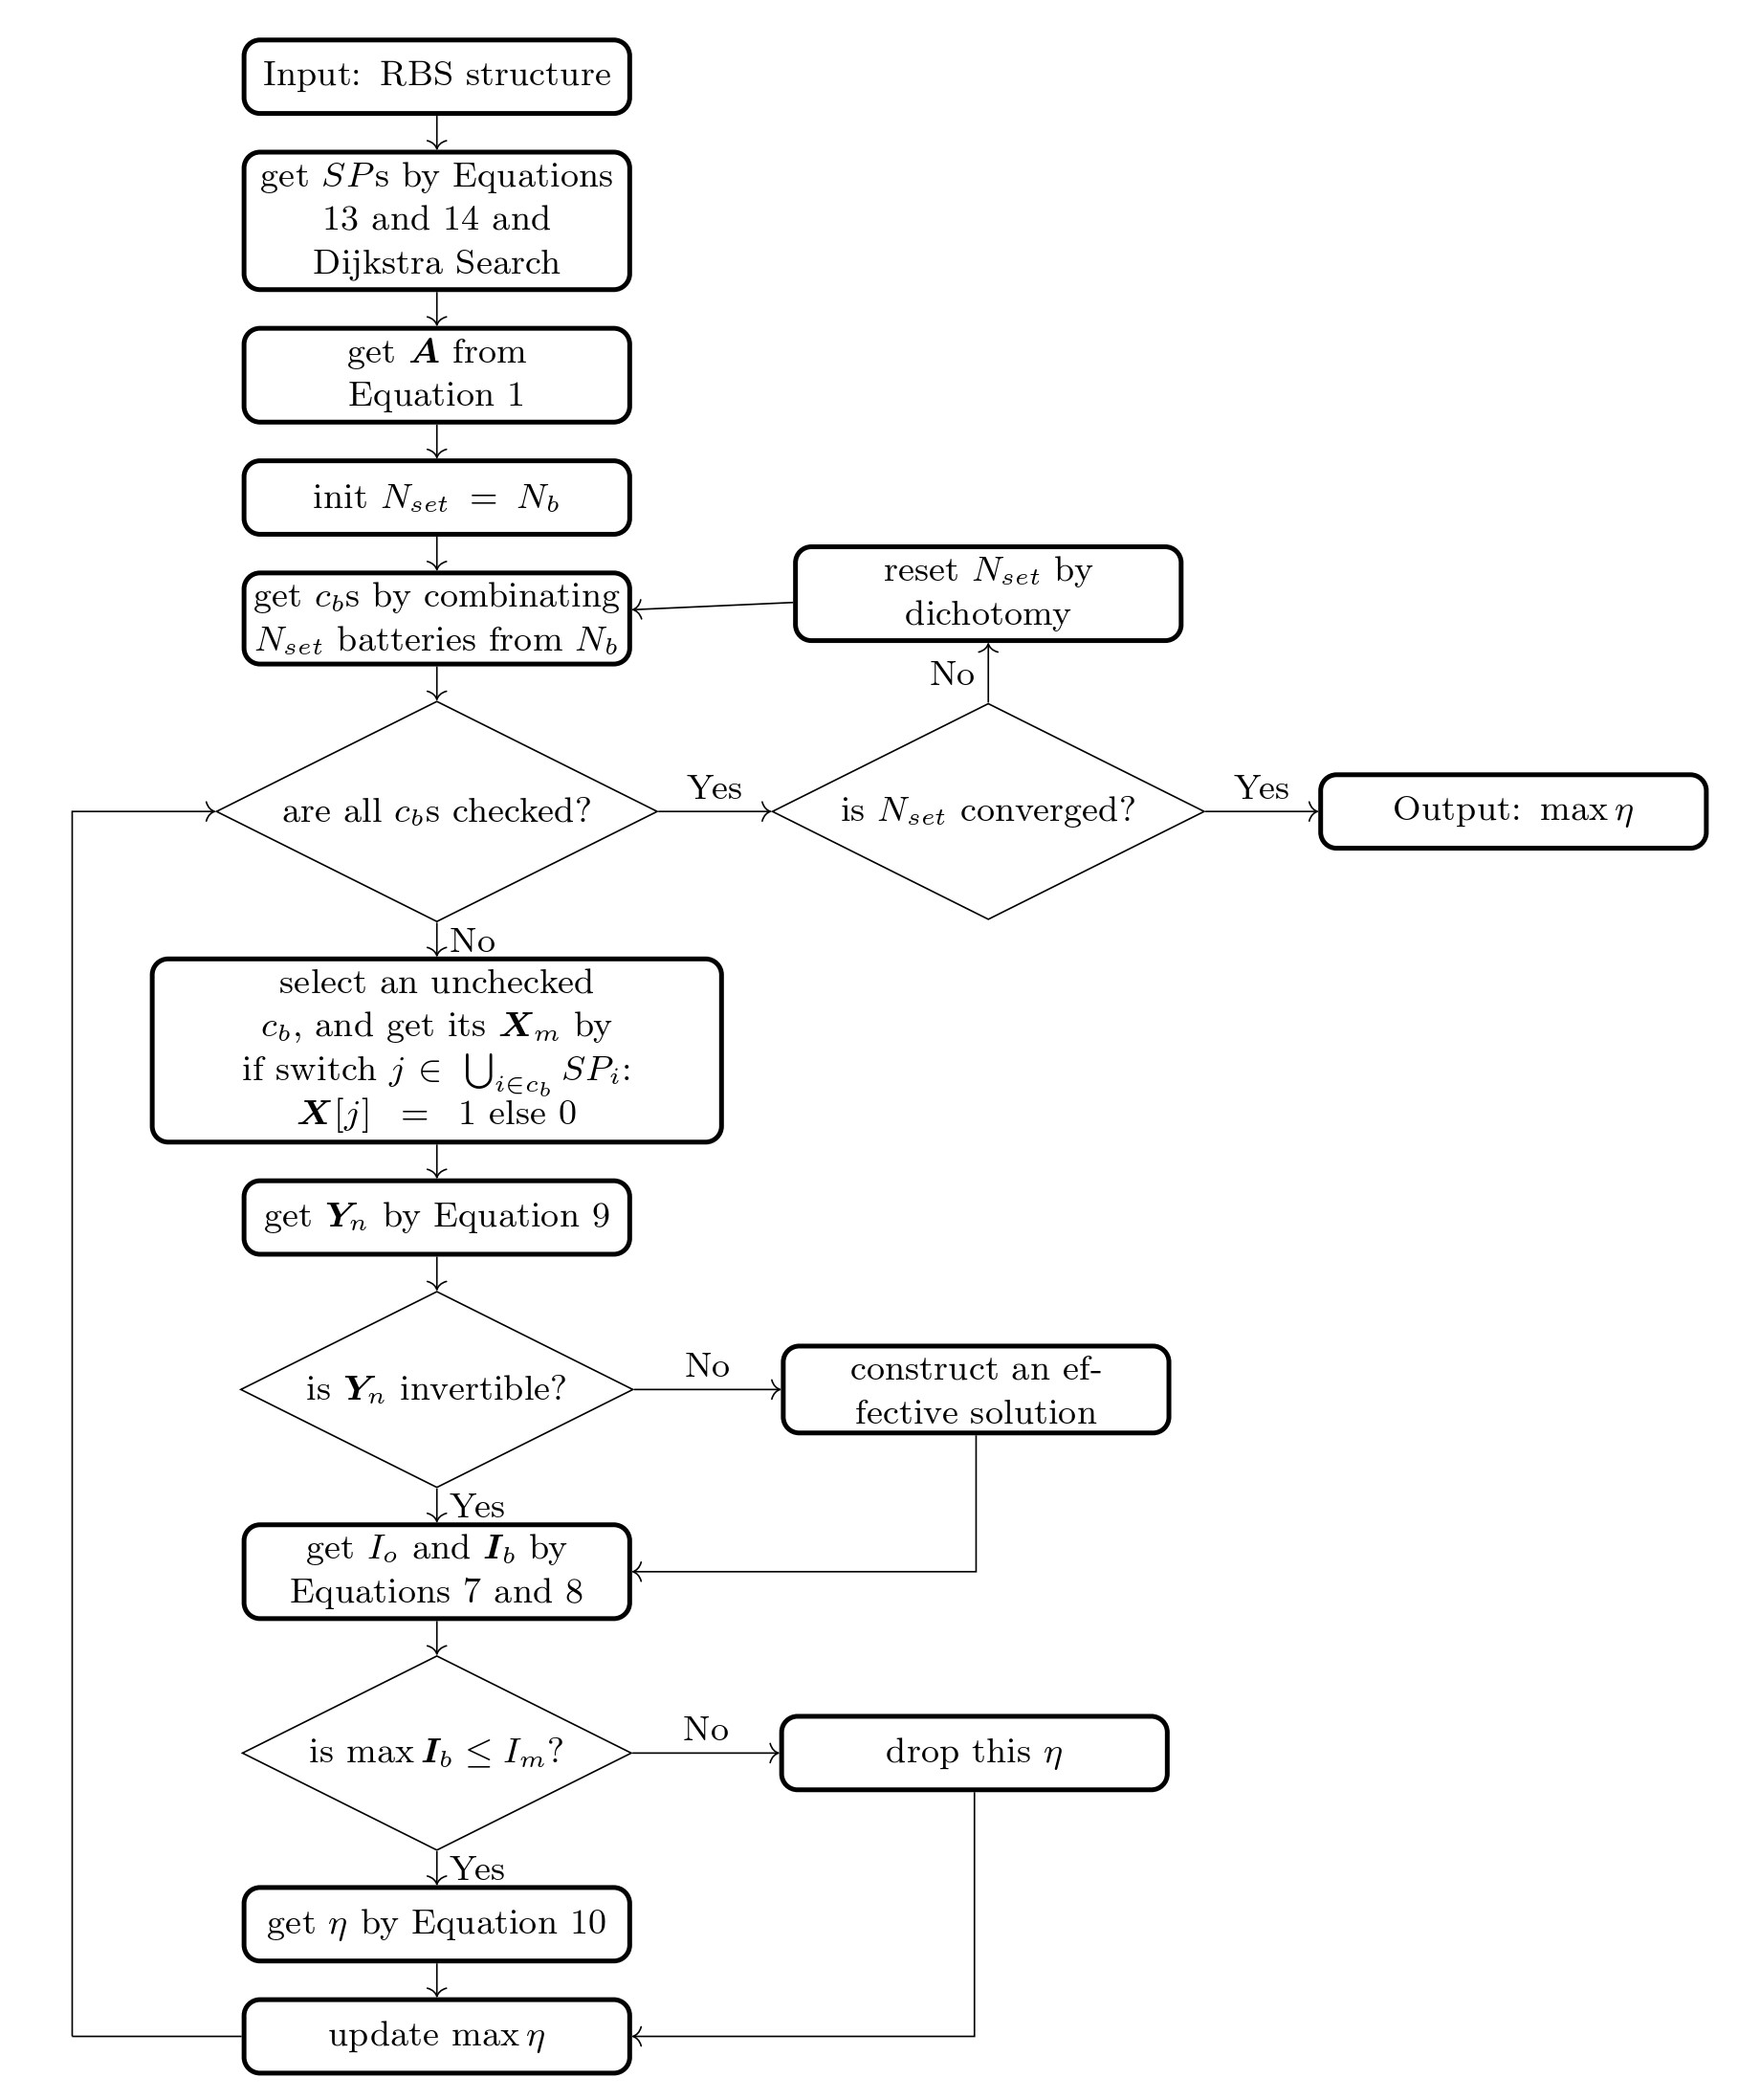
\includegraphics[width=\textwidth]{flowchart.jpg}
    \caption{The computational flowchart of the MAC for a given RBS.}\label{fig:flowchart}
\end{figure}

\section{Case Study}

\subsection{Structures}

\begin{figure}[htbp]
    \centering
    \begin{subfigure}[b]{0.2\textwidth}
        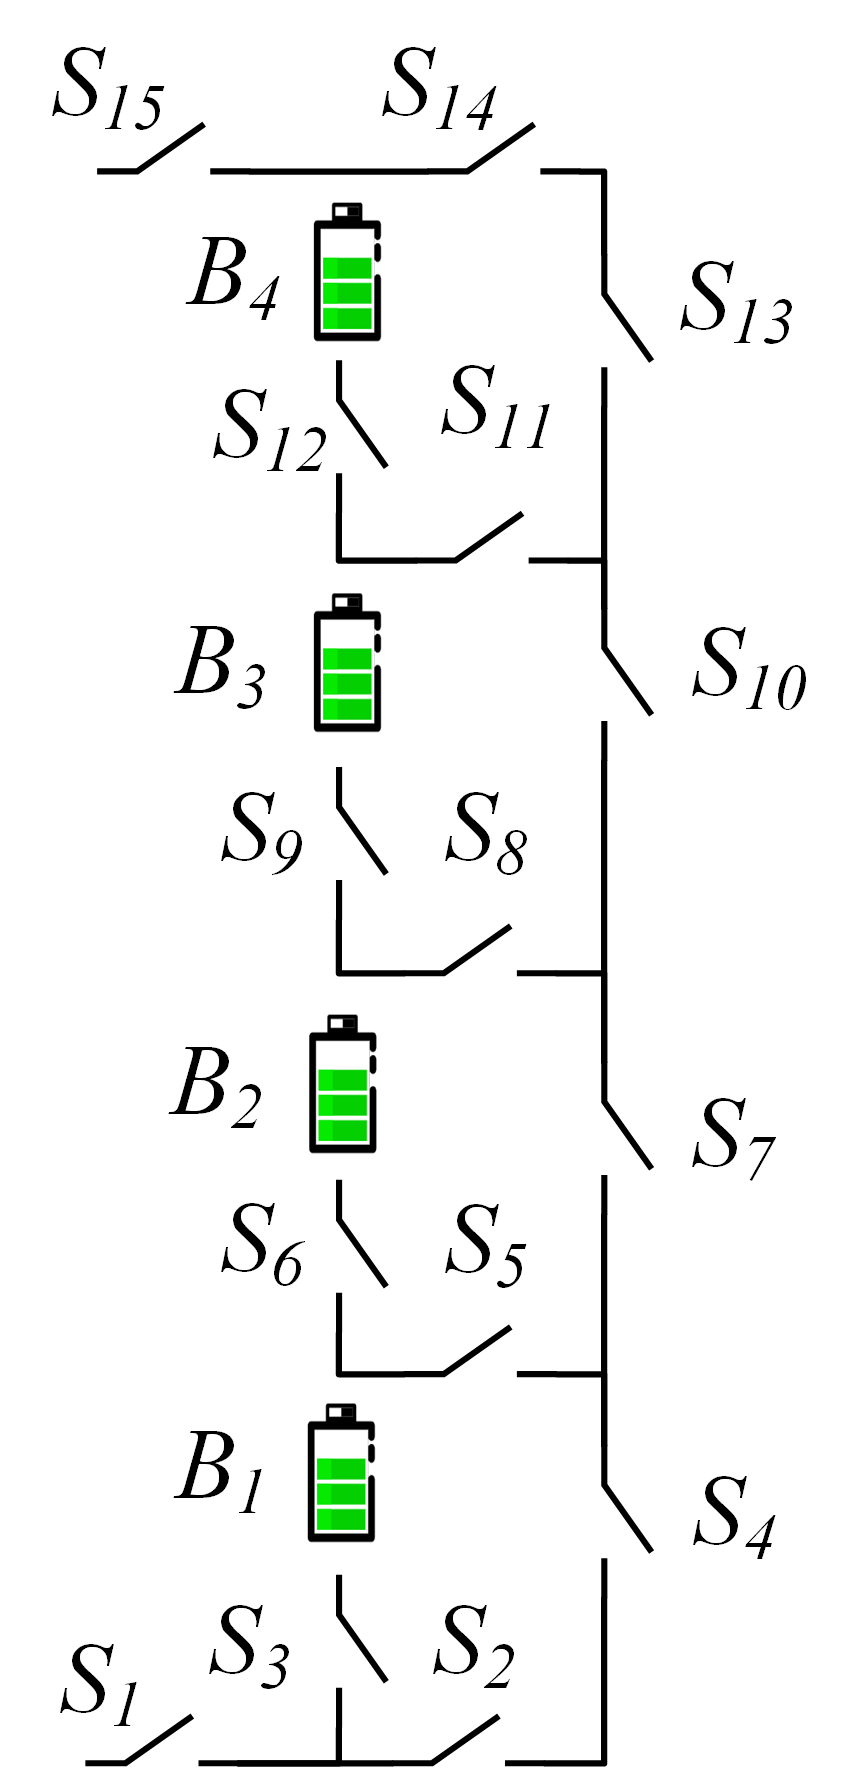
\includegraphics[width=\textwidth]{stru-L-origin.png}
        \caption{}
        \label{fig:study-stru-Lawson}
    \end{subfigure}
    \hspace{0.02\textwidth}
    \begin{subfigure}[b]{0.4\textwidth}
        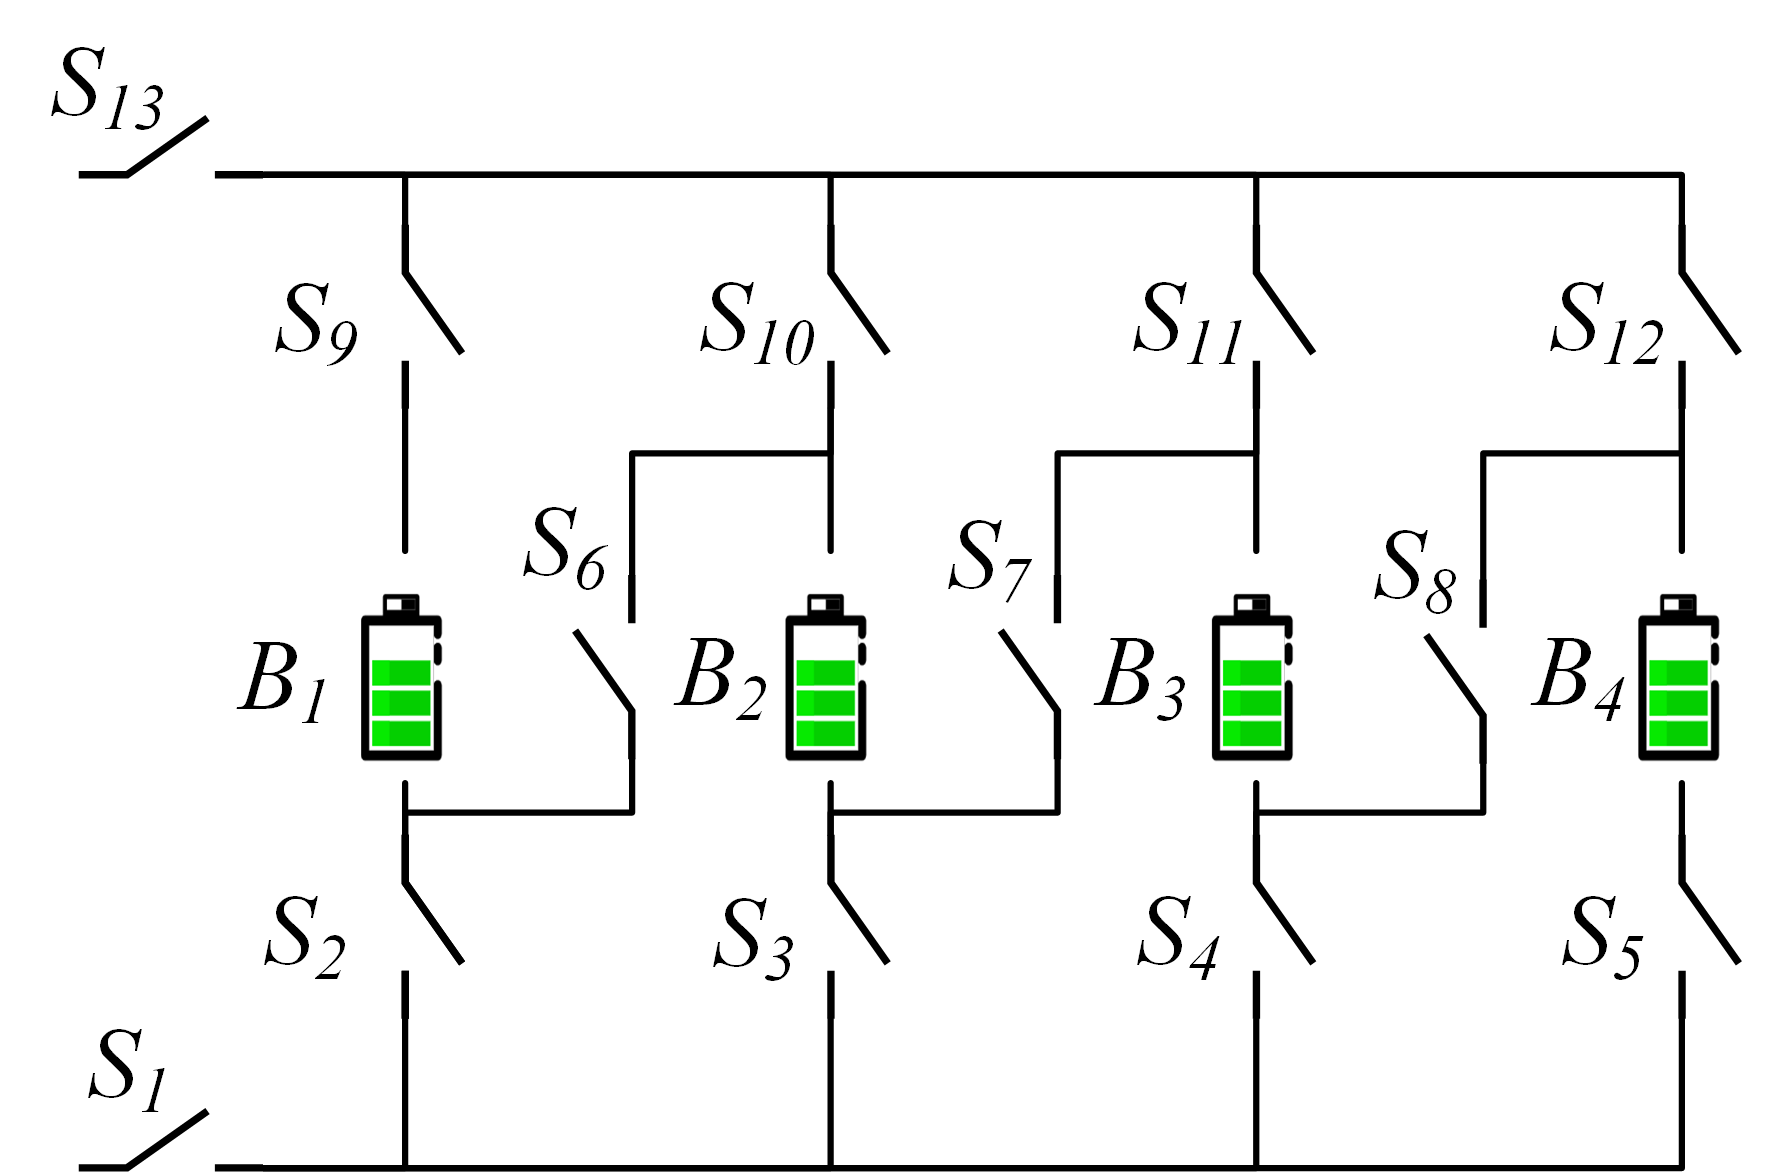
\includegraphics[width=\textwidth]{stru-V-origin.png}
        \caption{}
        \label{fig:study-stru-Visairo}
    \end{subfigure}
    \hspace{0.02\textwidth}
    \begin{subfigure}[b]{0.31\textwidth}
        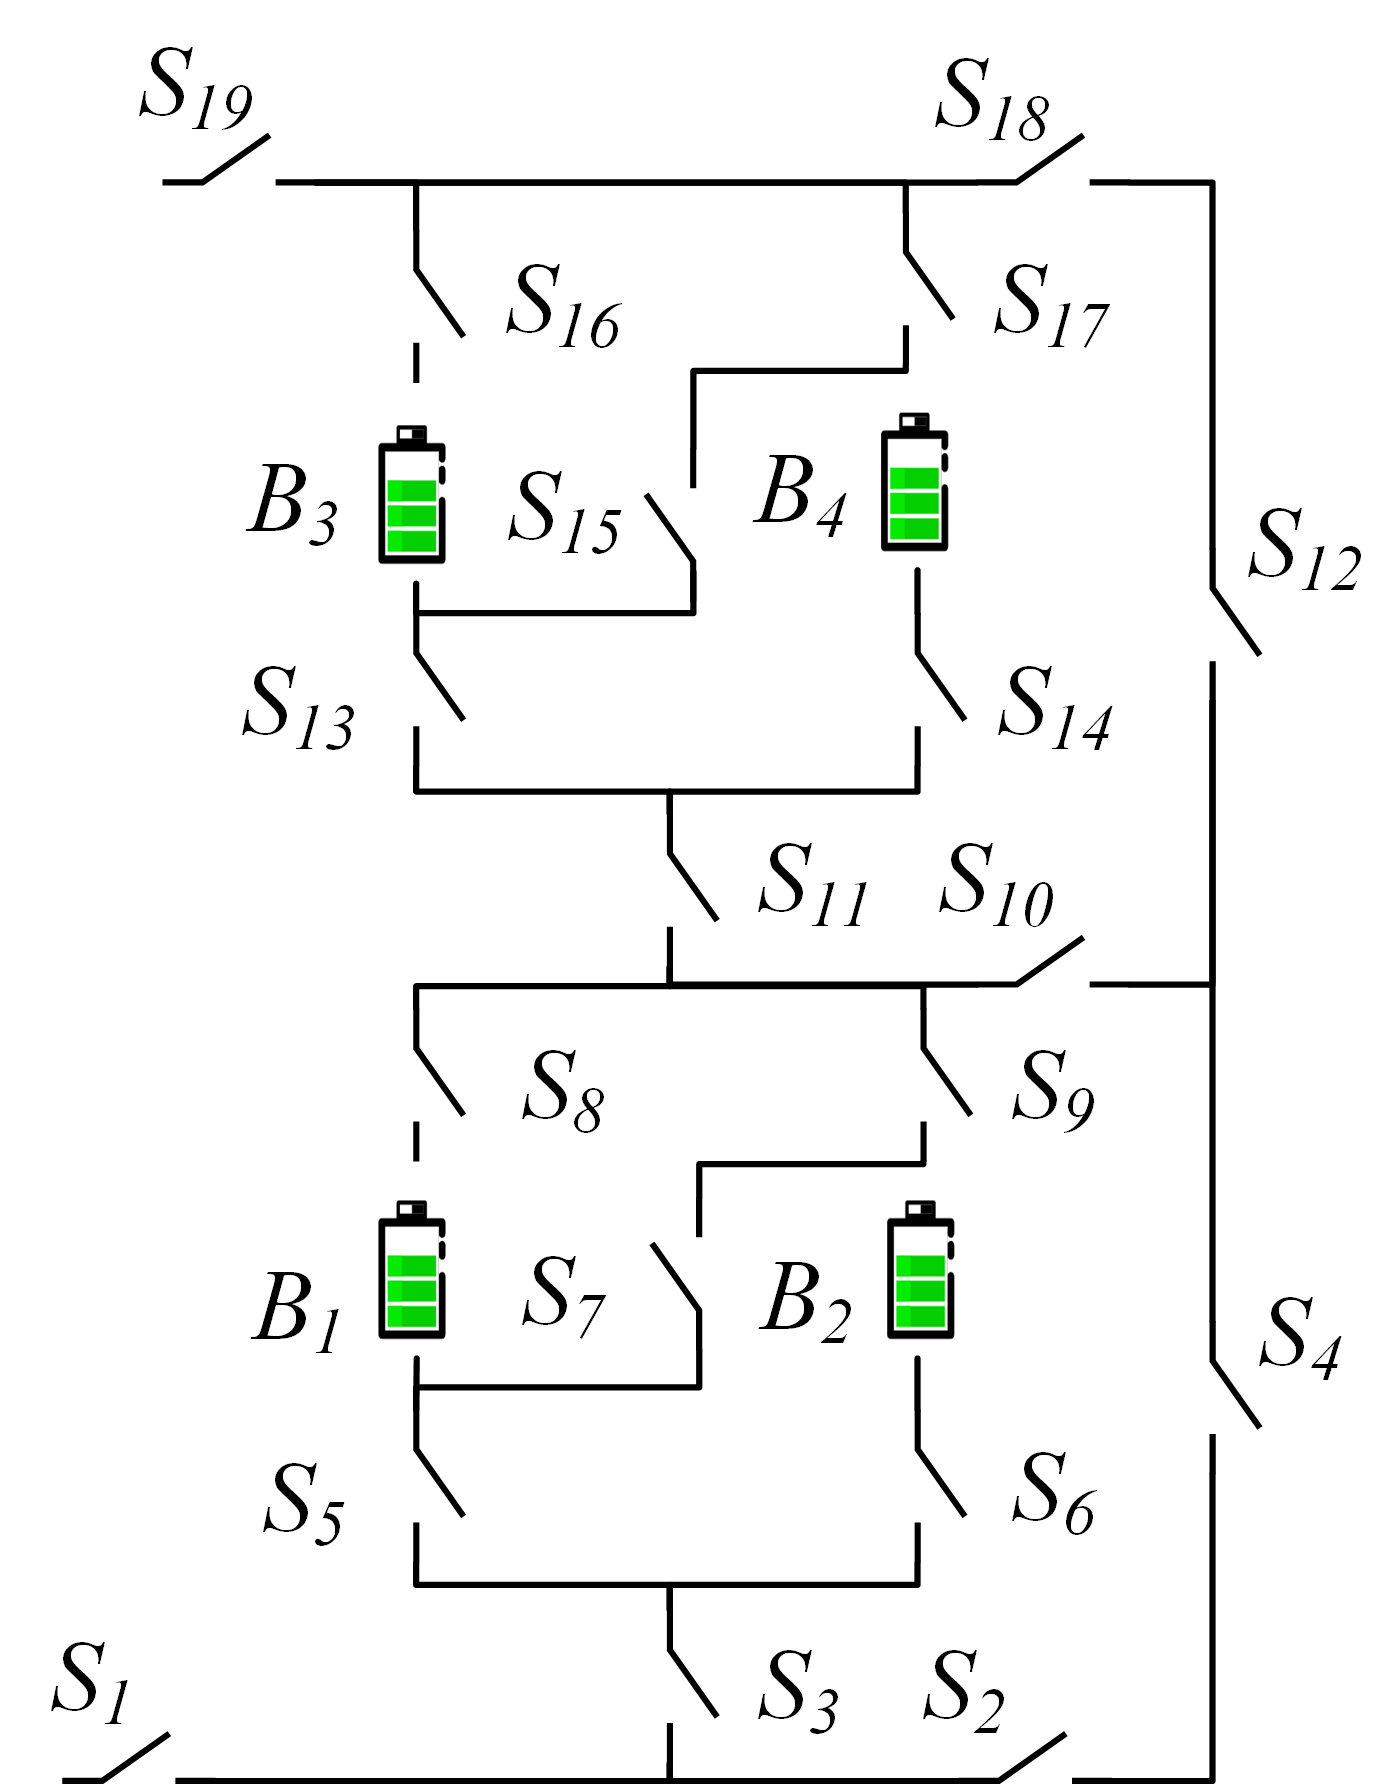
\includegraphics[width=\textwidth]{stru-my-origin.png}
        \caption{}
        \label{fig:study-stru-my}
    \end{subfigure}
    \caption{The 4-battery RBS structures proposed by (a)Lawson\cite{lawsonSoftwareConfigurableBattery2012}, (b)Visairo\cite{visairoReconfigurableBatteryPack2008} and (c)this paper.}
\end{figure}

Currently, two types of RBS structures have been proposed by Visairo et al. \cite{visairoReconfigurableBatteryPack2008} and Lawson et al. \cite{lawsonSoftwareConfigurableBattery2012}, both of which have been \replaced{practically used}{applied in practice}. 
The primary goal of Visairo's structure (Figure \ref{fig:study-stru-Visairo}) was to achieve dynamic adjustment of RBS output \added{power}; however, the isolation of unhealthy batteries was not sufficiently addressed \added{in their work}. 
\deleted{When batteries need to be isolated in the RBS of Visairo's structure, the methods for isolating them and the subsequent changes in RBS output warrant further investigation.}
Lawson et al. \replaced{designed the RBS structure shown in Figure \ref{fig:study-stru-Lawson} for the purpose of battery isolation}{conducted research on battery isolation in RBS and specifically designed the structure shown in Figure \ref{fig:study-stru-Lawson}}. 
This structure has the advantage of easily isolating batteries, but it cannot dynamically adjust the output current of RBS. 
Based on the structures of Visairo and Lawson, this paper presents a new structure, as shown in Figure \ref{fig:study-stru-my}\deleted{, which combines the advantages of both}.
By integrating the Visairo RBS structure into the Lawson RBS structure, the new structure not only allows the flexibility to switch the batteries between series, parallel, and mixed series-parallel modes, but also easily enables the isolation of highly degraded batteries from the RBS.
And their variations in output current under battery isolation conditions will be studied.
This RBS structure will be used to validate the effectiveness of the proposed method for calculating the MAC, and be compared with the Lawson's and Visairo's structure to illustrate its advantage on battery isolation.

\subsection{Result}

As shown in Figure \ref{fig:study-stru-my}, the new RBS structure consists of 4 batteries and 19 switches. 
The corresponding directed graph is depicted in Figure \ref{fig:study-dirgraph-my}, which is composed of a total of 18 nodes and 43 edges. 
Batteries $B_1$, $B_2$, $B_3$, and $B_4$ are denoted by green directed edges in the graph, while the 19 switches are represented by gray directed edges with bi-directional arrows. 
The external electrical load is treated as a directed edge from the cathode of the RBS (i.e., node 18) to the anode (i.e., node 1), as indicated by the blue directed edge in the graph.
Utilizing Equation \ref{eq:weight} and the Dijkstra algorithm, the $SP$s of the four batteries in the RBS structure of Figure \ref{fig:study-stru-my} are highlighted by red in Figures \ref{fig:sp1}-\ref{fig:sp4}.
Finally, the MAC calculation results of the structure in Figure \ref{fig:study-stru-my} are shown as Table \ref{tab:study-results-my} and Figure \ref{fig:study-results-my}, obtained by the greedy algorithm 1. % \ref{alg:greedy}.
Table \ref{tab:study-results-my} contains the switches states, the output current $I_o$, battery current $\bm{I}_b$ and ratio $\eta$ of the RBS structure with all batteries in good health when the RBS output reaches the MAC.
Figure \ref{fig:study-results-my} presents the corresponding circuit, with the red highlight indicating that current is flowing through the respective branches.

\begin{figure}[htbp]
    \centering
    \begin{subfigure}[b]{0.28\textwidth}
        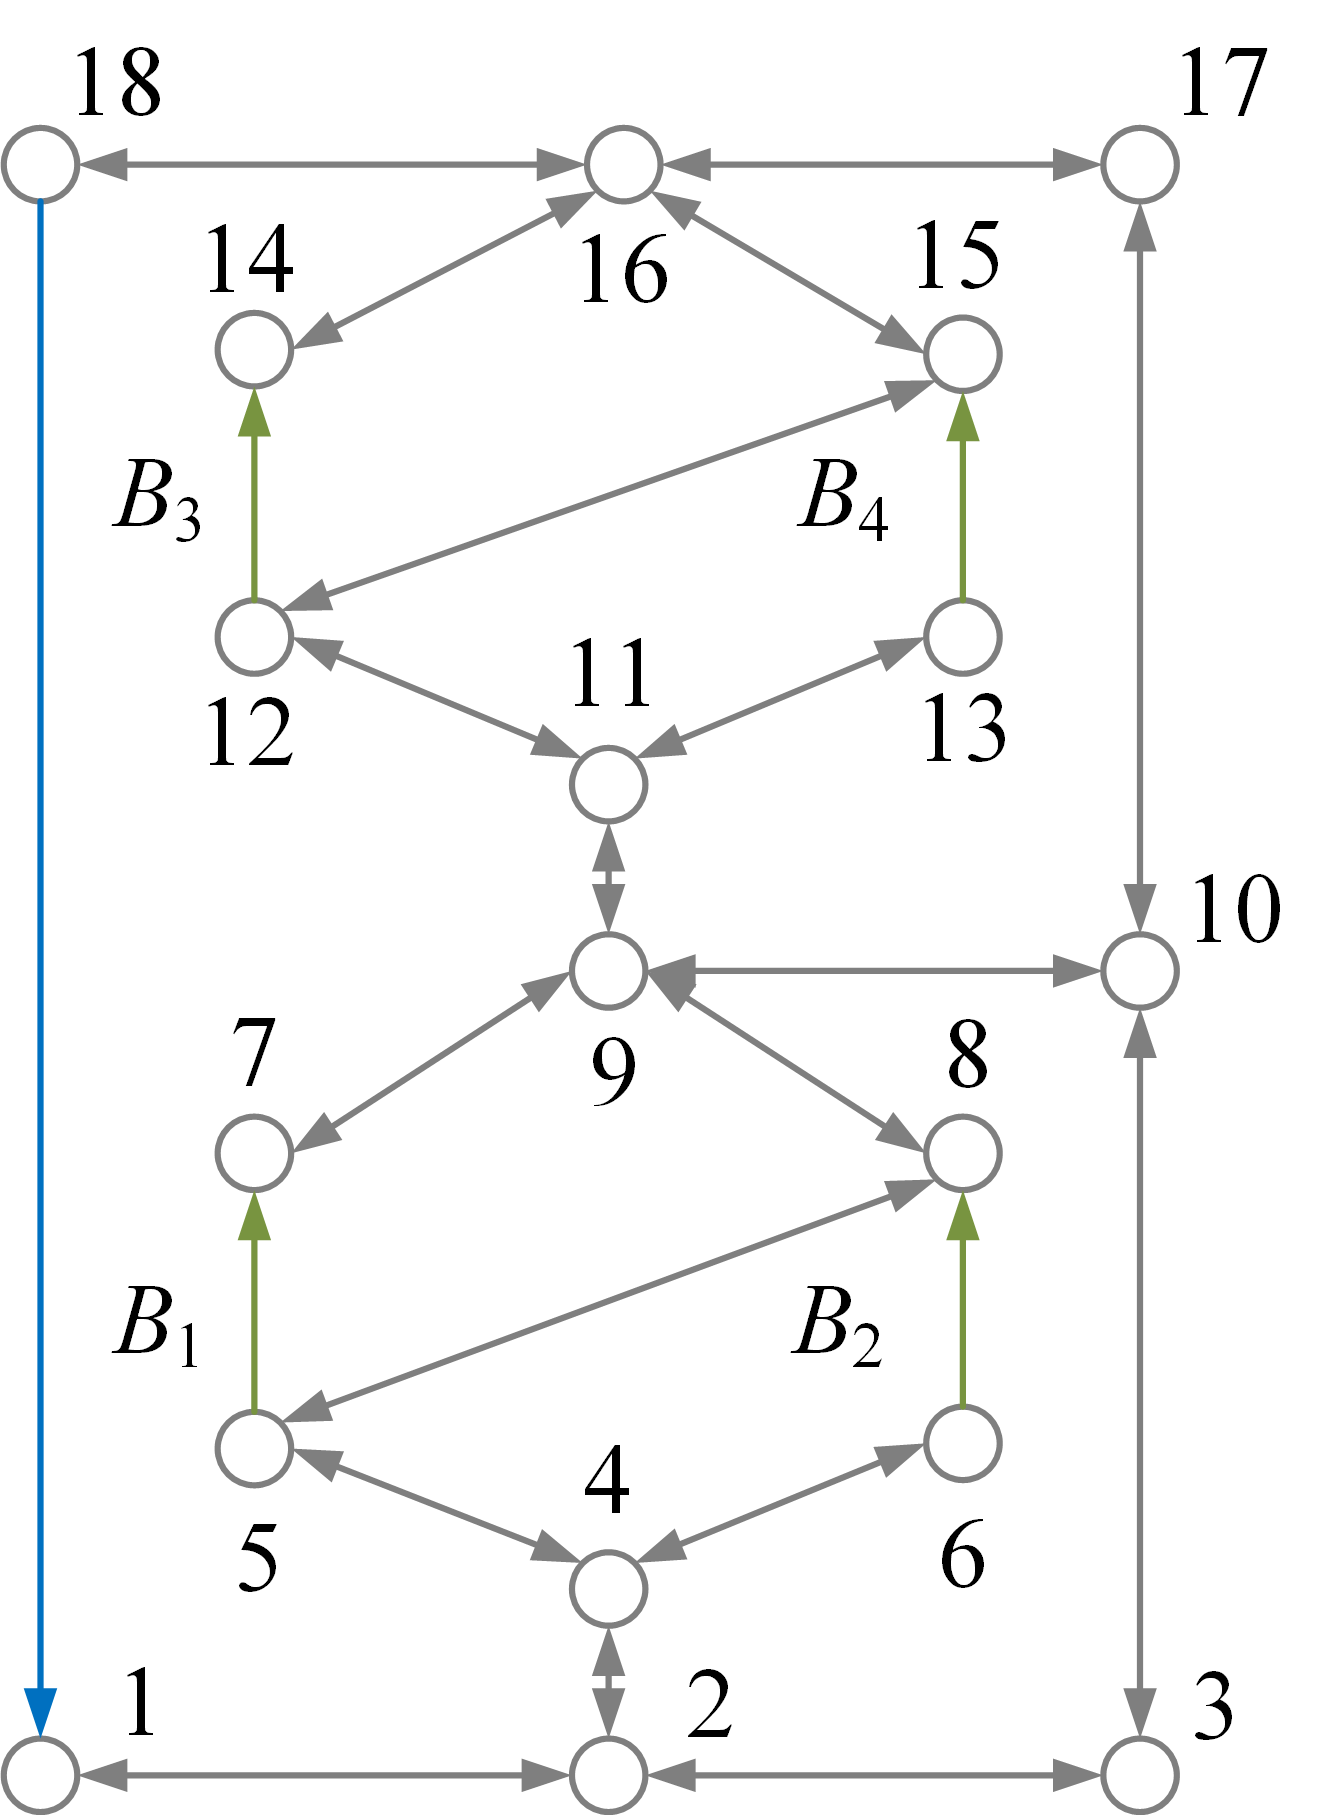
\includegraphics[width=\textwidth]{ef-topo.png}
        \caption{}
        \label{fig:study-dirgraph-my}
    \end{subfigure}
    \hspace{0.05\textwidth}
    \begin{subfigure}[b]{0.28\textwidth}
        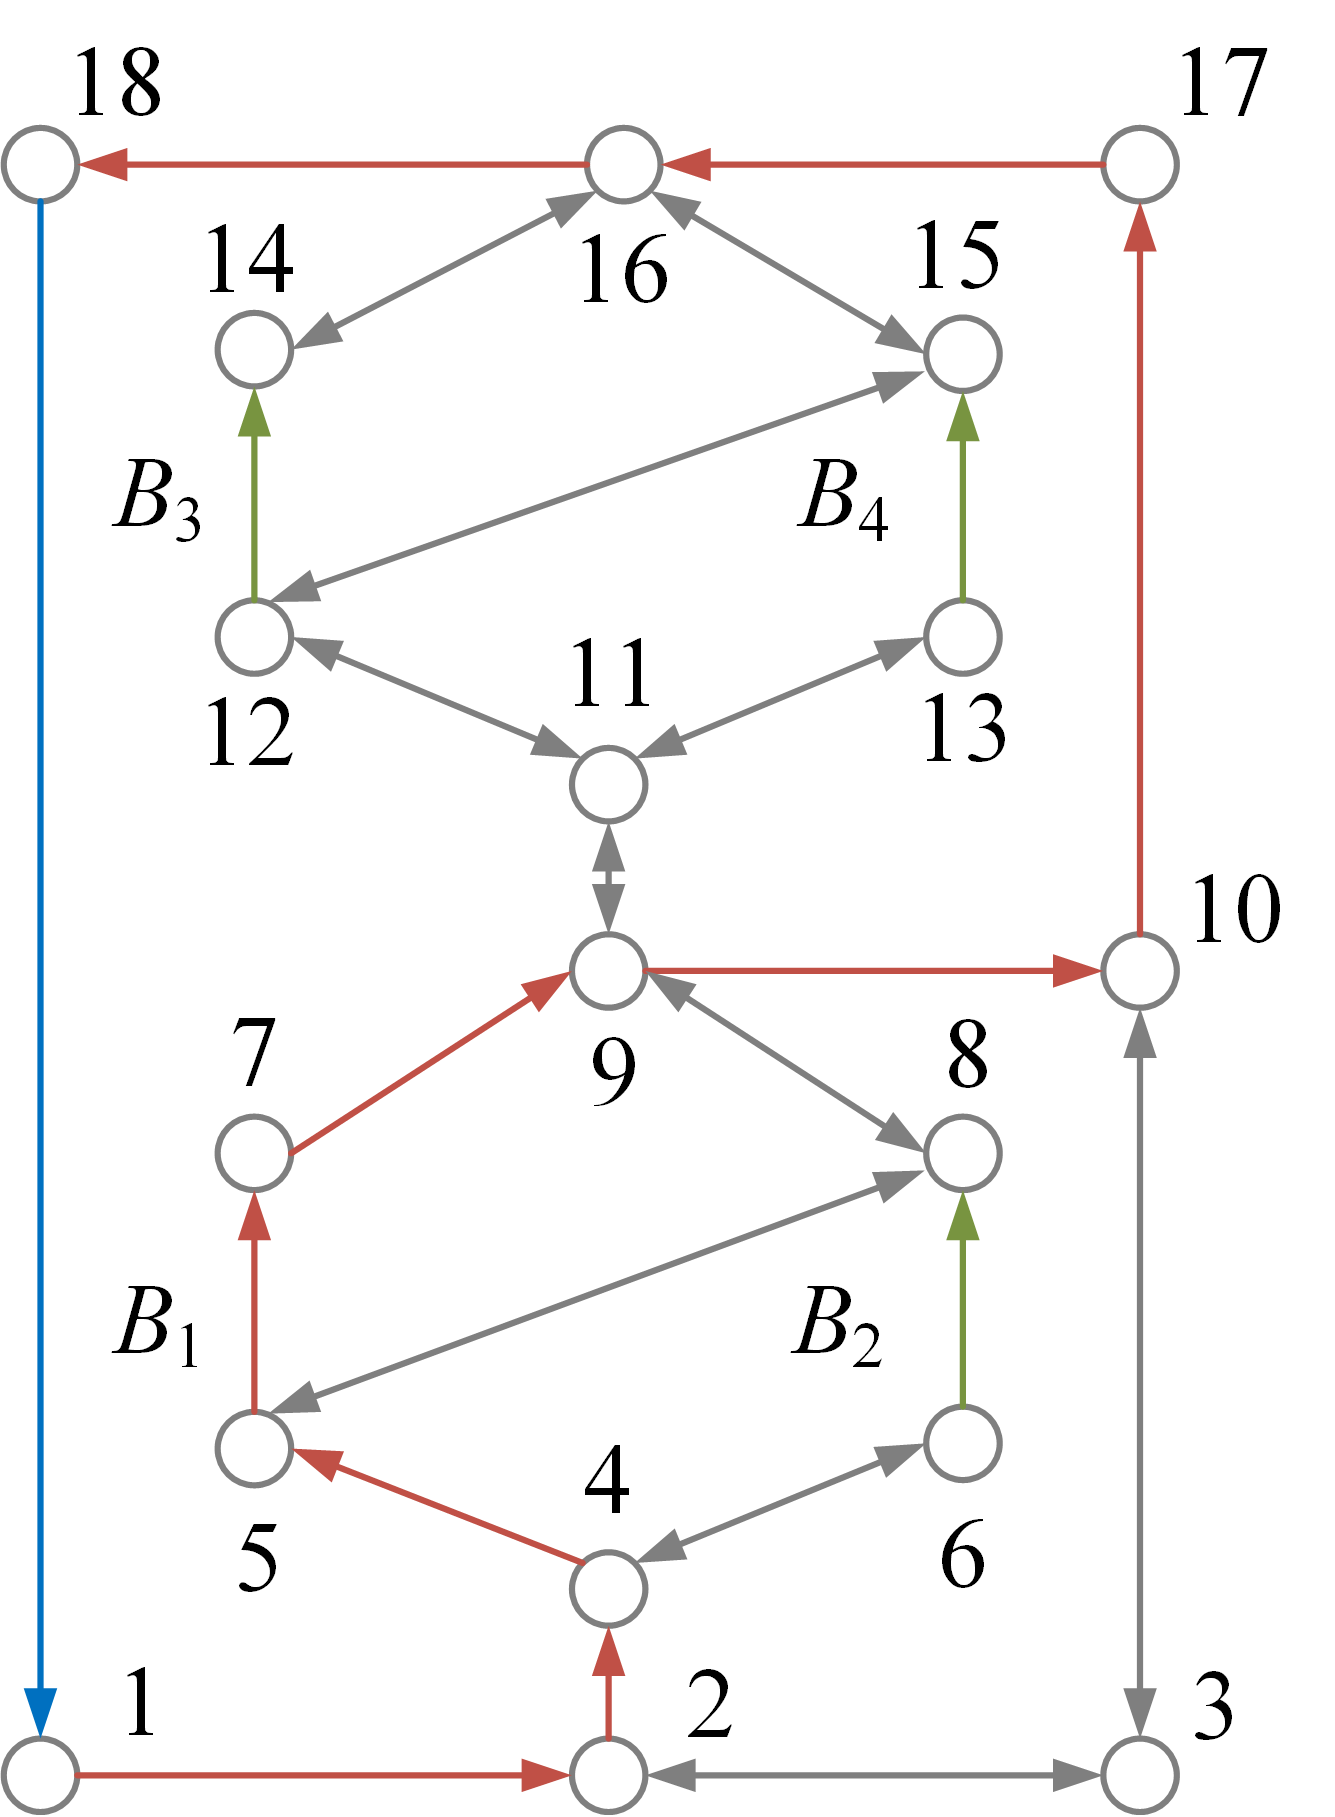
\includegraphics[width=\textwidth]{ef-sp1.png}
        \caption{}
        \label{fig:sp1}
    \end{subfigure}
    \hspace{0.05\textwidth}
    \begin{subfigure}[b]{0.28\textwidth}
        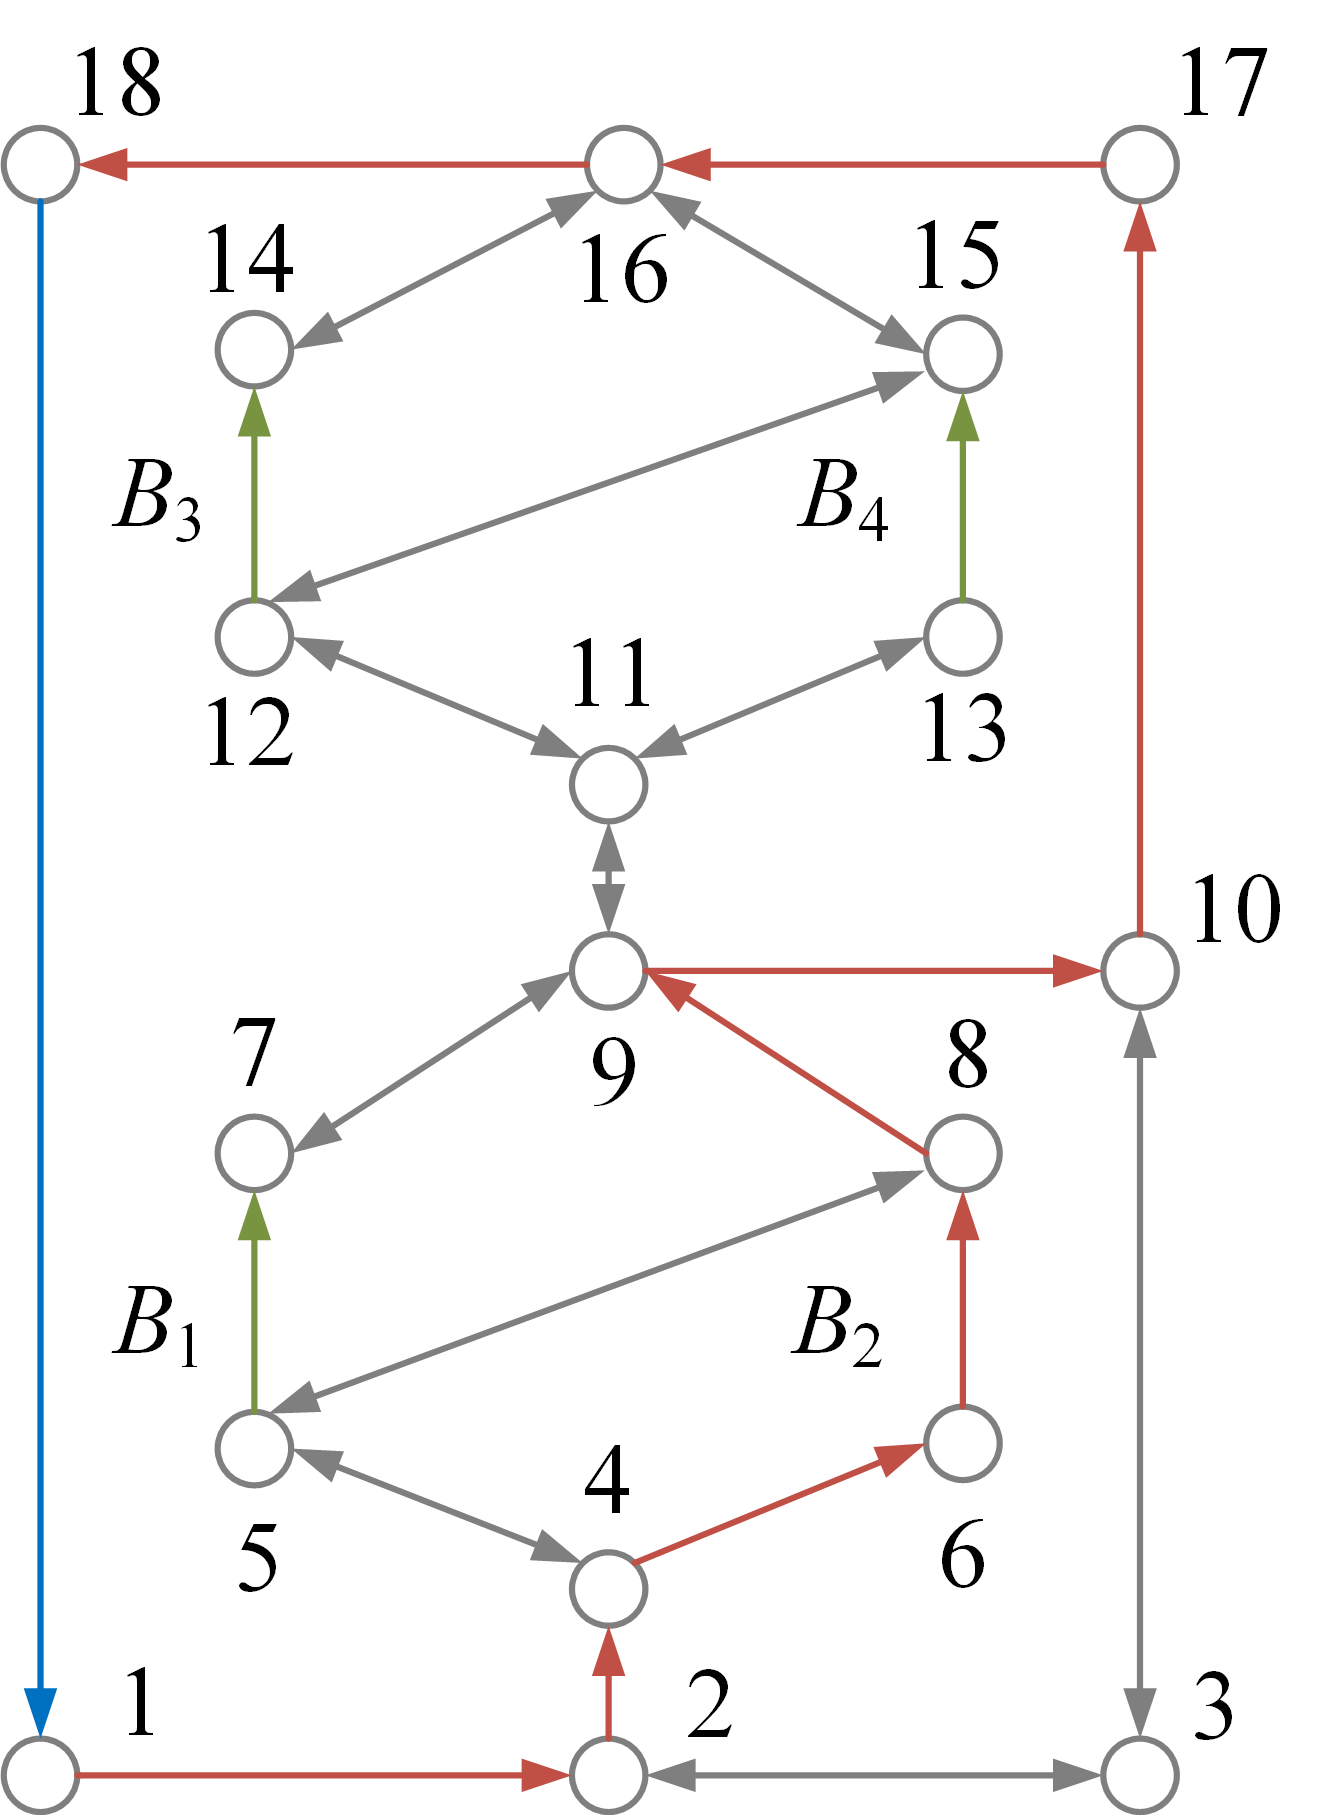
\includegraphics[width=\textwidth]{ef-sp2.png}
        \caption{}
        \label{fig:sp2}
    \end{subfigure}
    \\
    \begin{subfigure}[b]{0.28\textwidth}
        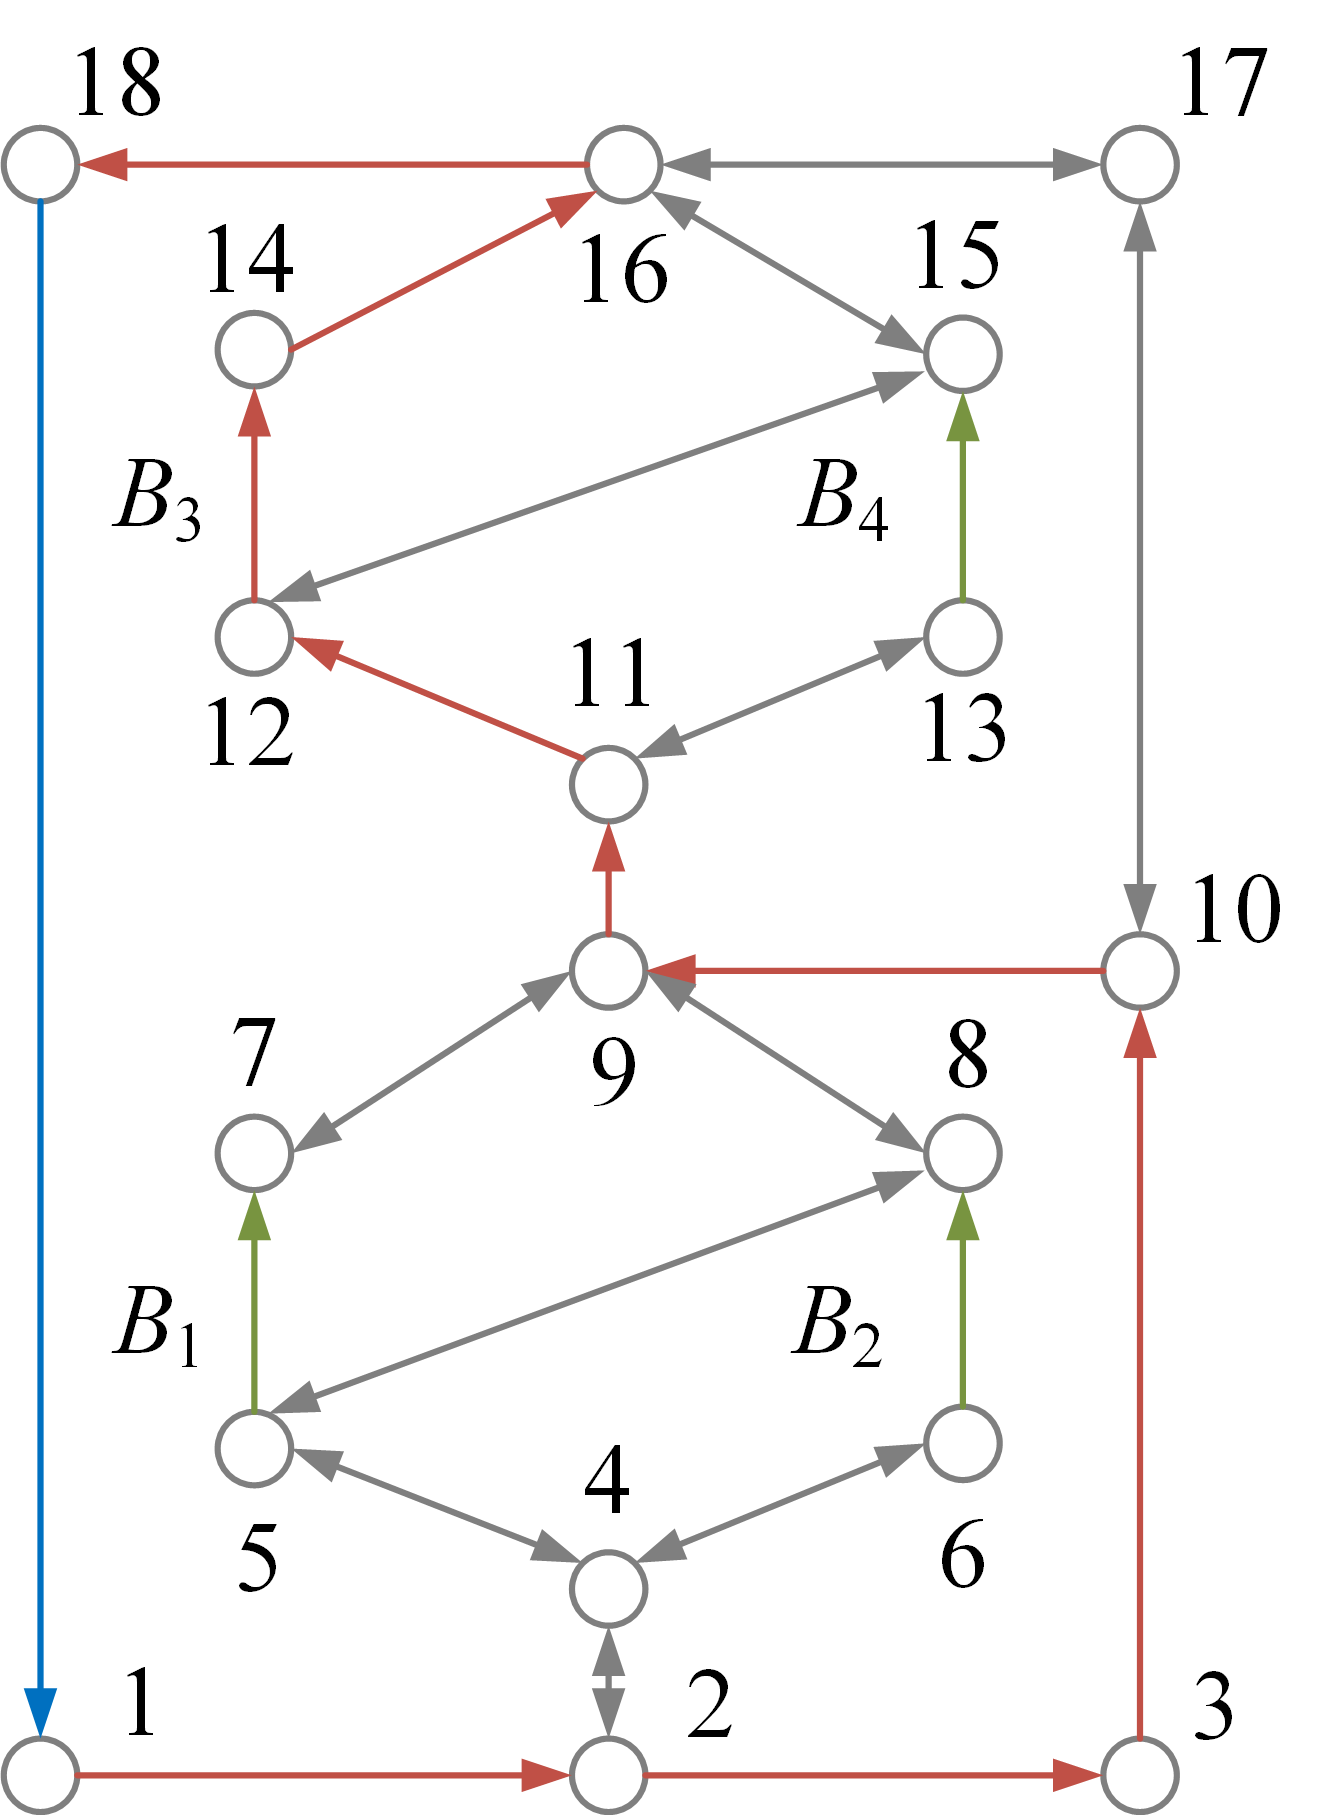
\includegraphics[width=\textwidth]{ef-sp3.png}
        \caption{}
        \label{fig:sp3}
    \end{subfigure}
    \hspace{0.05\textwidth}
    \begin{subfigure}[b]{0.28\textwidth}
        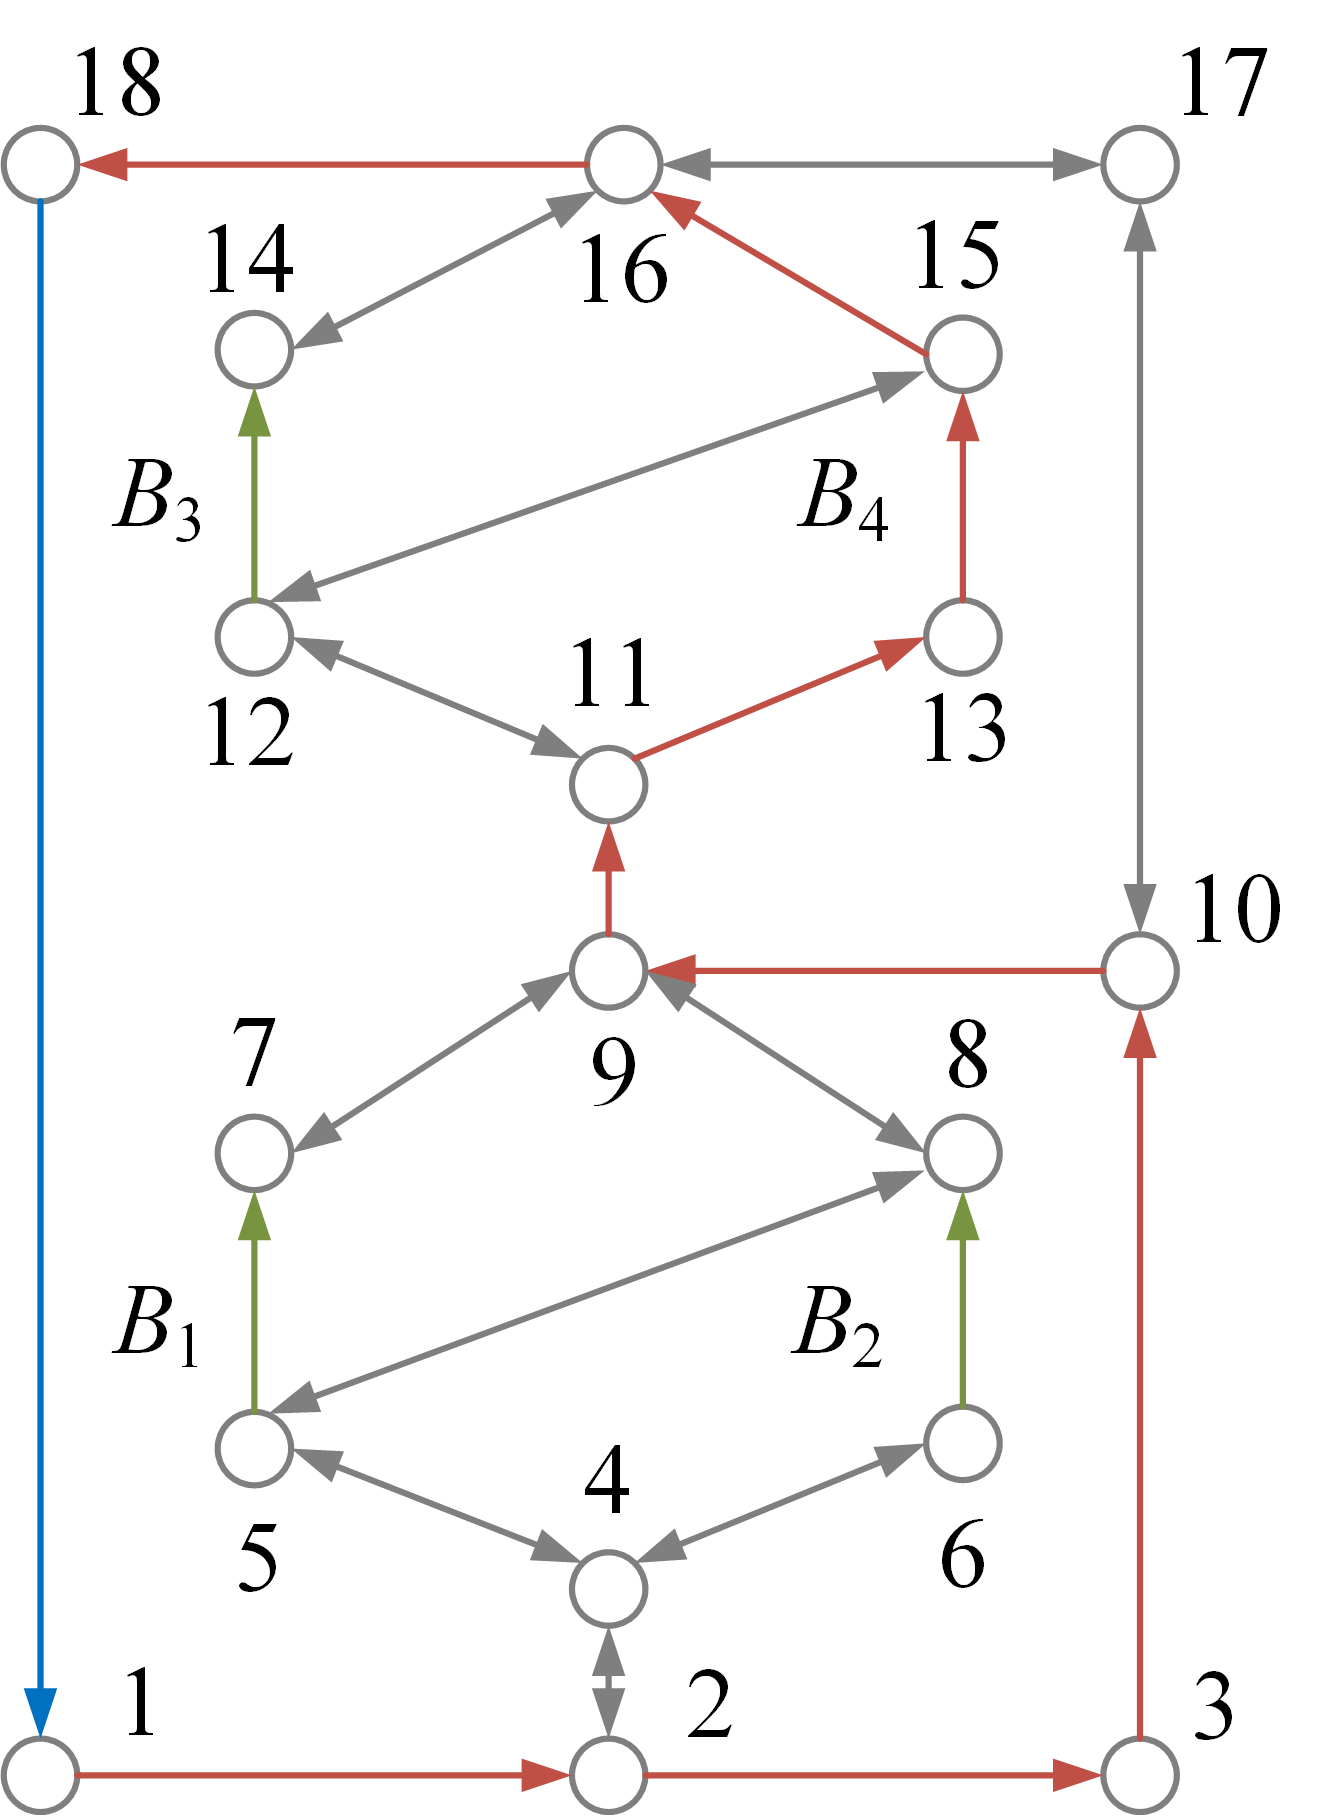
\includegraphics[width=\textwidth]{ef-sp4.png}
        \caption{}
        \label{fig:sp4}
    \end{subfigure}
    \hspace{0.05\textwidth}
    \begin{subfigure}[b]{0.28\textwidth}
        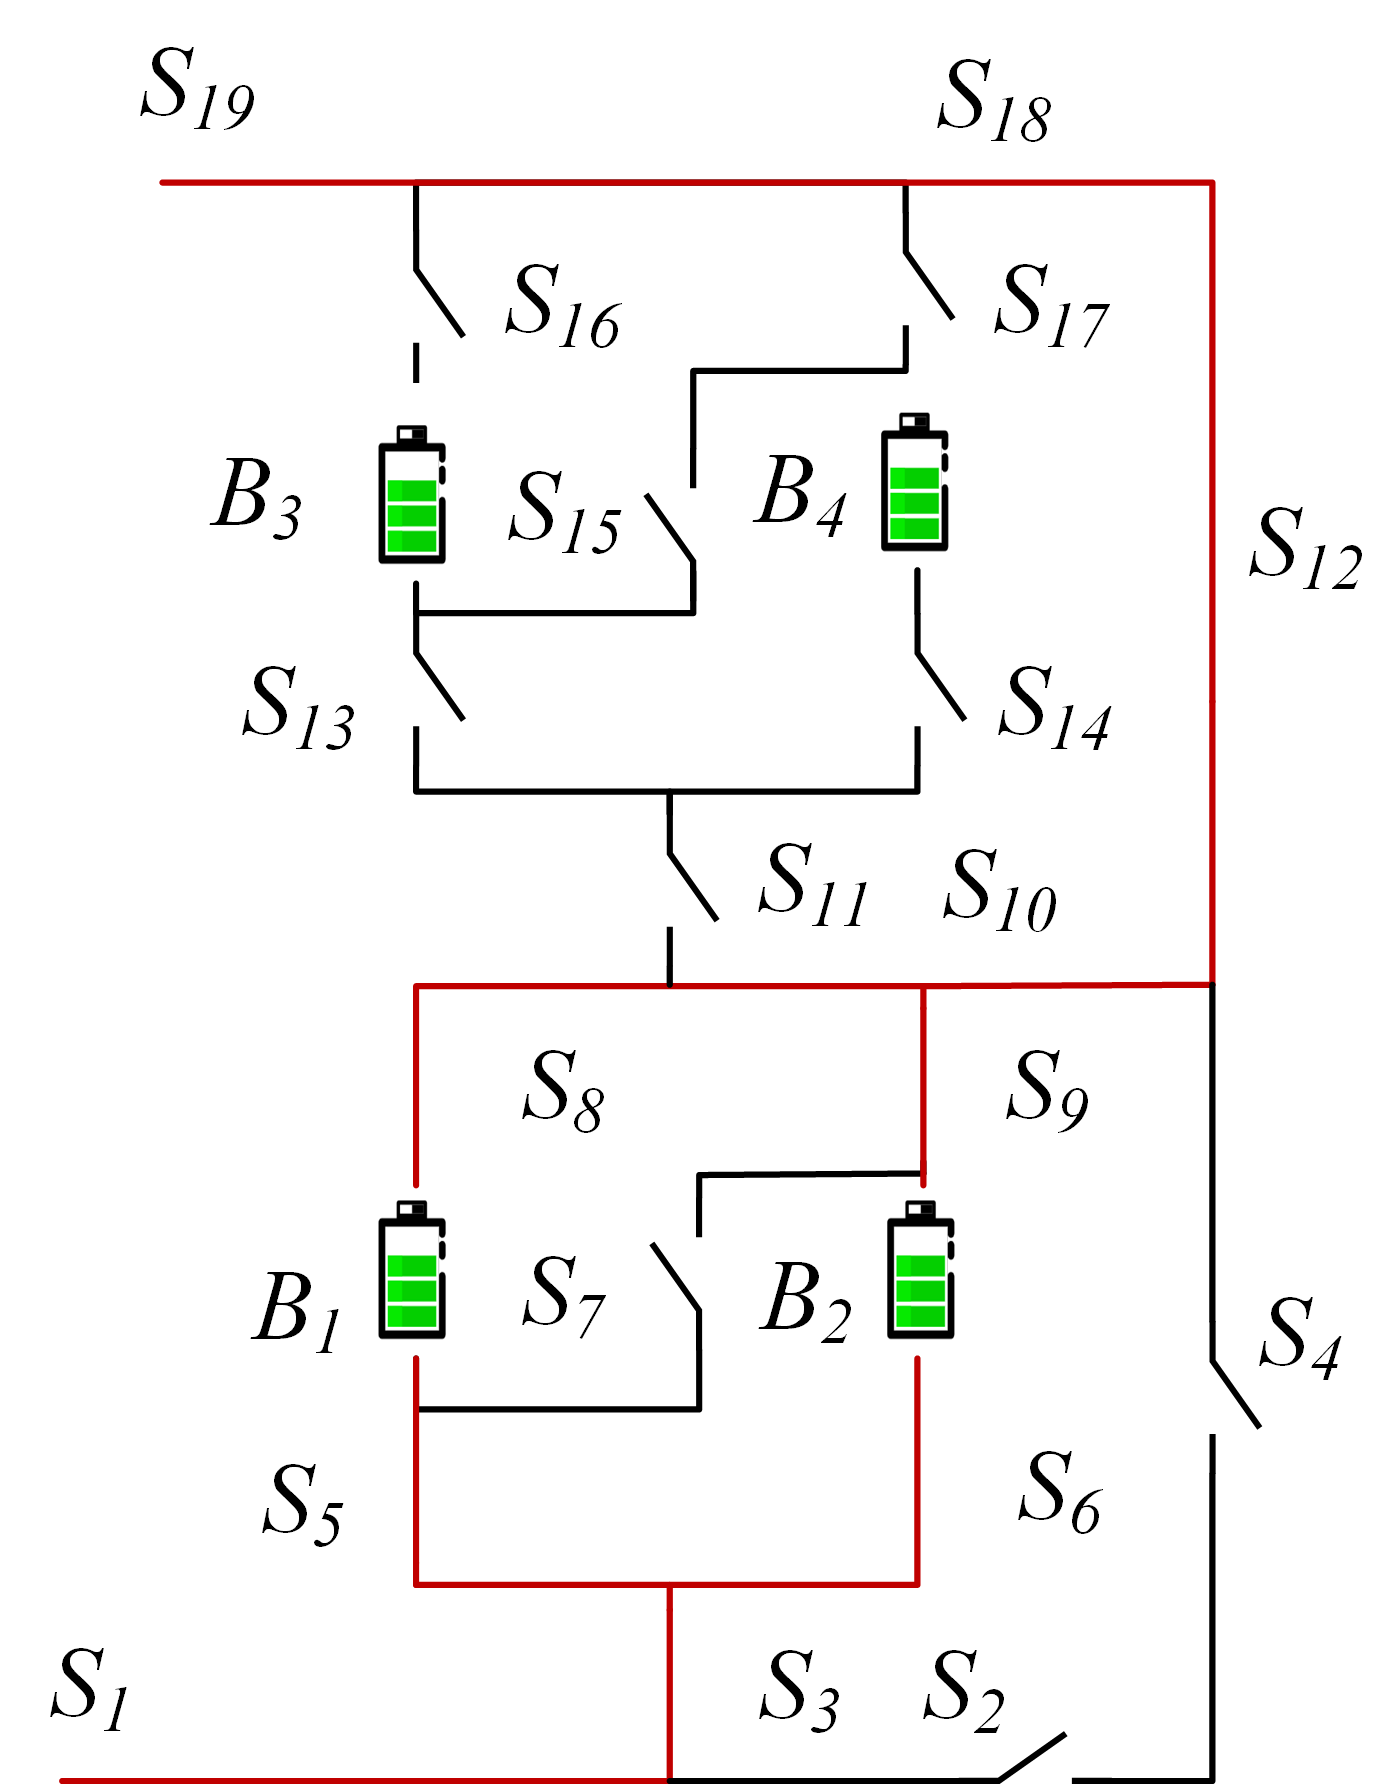
\includegraphics[width=\textwidth]{ef-mac.png}
        \caption{}
        \label{fig:study-results-my}
    \end{subfigure}
    \caption{
        For the RBS structure in Figure \ref{fig:study-stru-my}, 
        (a)its directed graph 
        and the $SP$s (highlighted in red) of battery (b)$B_1$, (c)$B_2$, (d)$B_3$, (e)$B_4$.
        (f)The circuit of the RBS with its output reaching the MAC.
        }
    \label{fig:all-results-my}
\end{figure}

\begin{table}[htbp]
  \centering
    \caption{MAC Calculating result of the 4-battery RBS structure in Figure \ref{fig:study-stru-my}.}
    \begin{tabular}{cc}
    \toprule
        Structure & Figure \ref{fig:study-stru-my} with 4 batteries and 19 switches  \\
    \midrule
    Switch ON & $S_1$,$S_3$,$S_5$,$S_6$,$S_8$,$S_9$,$S_{10}$,$S_{12}$,$S_{18}$,$S_{19}$ \\
    $I_o$ & $2u_b/(2R_o+r_b)$ \\
    $\bm{I}_b$ & $[u_b/(2R_o+r_b),u_b/(2R_o+r_b),0,0]$ \\
    \added{$\max$}$\eta$     & 2 \\
    \bottomrule
    \end{tabular}
  \label{tab:study-results-my}
\end{table}

Similarly, the MAC calculation results of the structures in Figures \ref{fig:study-stru-Lawson} and \ref{fig:study-stru-Visairo} are shown as Table \ref{tab:study-results-Lawson} and Table \ref{tab:study-results-Visairo}, respectively.
\added{
In order to verify and compare the results from the greedy algorithm, we also utilized a brute force algorithm that go through all possible switch states to calculate the MAC of the same three RBS. 
For a given RBS structure with $N_s$ switches, the final $\max$ $\eta$ is the maximum of $\eta$s from all $2^{N_s}$ reconfigured structures.
The final results are the same as the results shown in Tables \ref{tab:study-results-my}-\ref{tab:study-results-Visairo}.
It is worth noting that the method used the greedy algorithm only calculated 7, 11, and 1 reconfigured structures for the RBS structure in Figures \ref{fig:study-stru-my}, \ref{fig:study-stru-Lawson}, \ref{fig:study-stru-Visairo}, respectively. 
While for the same RBS, the method counted all possible switch states computed $2^{19}$, $2^{15}$, and $2^{13}$ structures, respectively.
}

\begin{table}[htbp]
  \centering
    \caption{MAC Calculating result of the 4-battery RBS structure in Figure \ref{fig:study-stru-Lawson}.}
    \begin{tabular}{cc}
    \toprule
        Structure & Figure \ref{fig:study-stru-Lawson} with 4 batteries and 15 switches  \\
    \midrule
    Switch ON & $S_1$,$S_3$,$S_5$,$S_7$,$S_{10}$,$S_{13}$,$S_{14}$,$S_{15}$ \\
    $I_o$ & $u_b/(R_o+r_b)$ \\
    $\bm{I}_b$ & $[u_b/(R_o+r_b),0,0,0]$ \\
    \added{$\max$}$\eta$     & 1 \\
    \bottomrule
    \end{tabular}
  \label{tab:study-results-Lawson}
\end{table}

\begin{table}[htbp]
  \centering
    \caption{MAC Calculating result of the 4-battery RBS structure in Figure \ref{fig:study-stru-Visairo}.}
    \begin{tabular}{cc}
    \toprule
        Structure & Figure \ref{fig:study-stru-Visairo} with 4 batteries and 13 switches  \\
    \midrule
    Switch ON & $S_1$,$S_2$,$S_3$,$S_4$,$S_5$,$S_9$,$S_{10}$,$S_{11}$,$S_{12}$,$S_{13}$ \\
    $I_o$ & $4u_b/(4R_o+r_b)$ \\
    $\bm{I}_b$ & $[u_b/(4R_o+r_b),u_b/(4R_o+r_b),u_b/(4R_o+r_b),u_b/(4R_o+r_b)]$ \\
    \added{$\max$}$\eta$     & 4 \\
    \bottomrule
    \end{tabular}
  \label{tab:study-results-Visairo}
\end{table}

Furthermore, the RBS \replaced{with}{under the scenario of} isolated batteries is taken into consideration and calculated. 
The MAC calculation results for the three structures under study, with varying numbers of isolated batteries, are presented in Table \ref{tab:isolated_mac}. 
Figures \ref{fig:my-isolated-1}-\ref{fig:my-isolated-3} illustrate the corresponding switch control schemes for the new structure proposed in this paper under different isolated battery conditions.
\deleted{The characteristics of these three structures in the context of battery isolation will be discussed in the next subsection.}

\begin{table}[htbp]
    \centering
    \caption{
      The variation of MAC with the number of isolated batteries for different RBS structures, including the structure proposed by Lawson et al., Visairo et al. , and the structure proposed in this paper.
      }
      \label{tab:isolated_mac}
      \begin{tabular}{cccc}
      \toprule
      \multirow{2}[4]{*}{number of isolated batteries} & \multicolumn{3}{c}{$\eta$ of RBS structure} \\
  \cmidrule{2-4}          & our  & Visairo's  & Lawson's  \\
      \midrule
      0     & 2     & 4     & 1 \\
      1     & 2     & 3     & 1 \\
      2     & 2$^{\mathrm{a}}$ or 1$^{\mathrm{b}}$ & 2     & 1 \\
      3     & 1     & 1     & 1 \\
      \bottomrule
      \end{tabular}
      \\
      \footnotesize{$^{\mathrm{a}}$ isolate two batteries within the same substructure, as shown in Figure \ref{fig:my-isolated-2b}}\\
      \footnotesize{$^{\mathrm{b}}$ isolate one battery in each of the two substructures, as shown in Figure \ref{fig:my-isolated-2w}}
  \end{table}
  
  
  \begin{figure}[htbp]
      \centering
      \begin{subfigure}[b]{0.31\textwidth}
          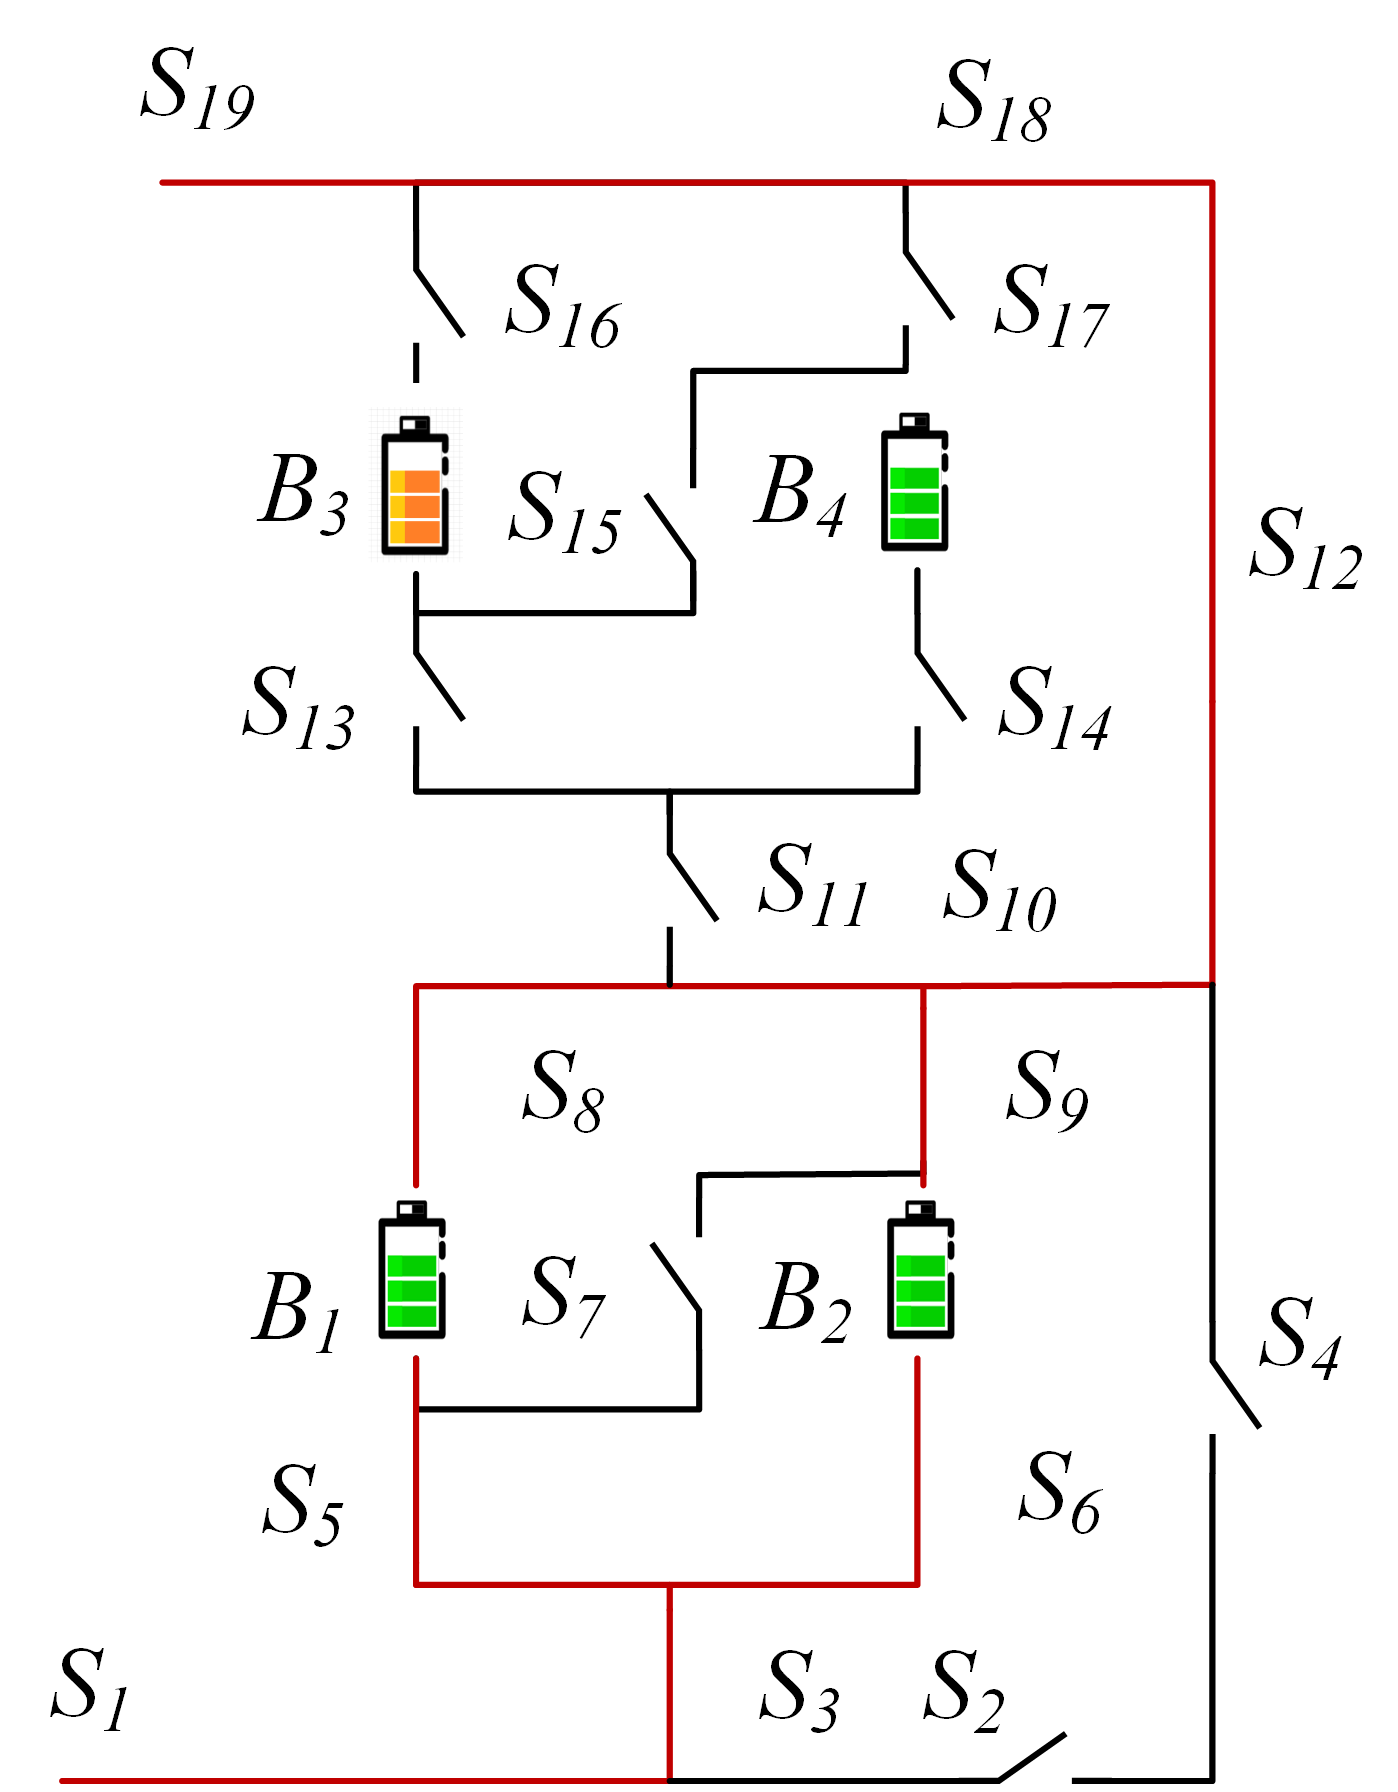
\includegraphics[width=\textwidth]{my-isolated-1.png}
          \caption{}
          \label{fig:my-isolated-1}
      \end{subfigure}
      \hspace{0.02\textwidth}
      \begin{subfigure}[b]{0.31\textwidth}
          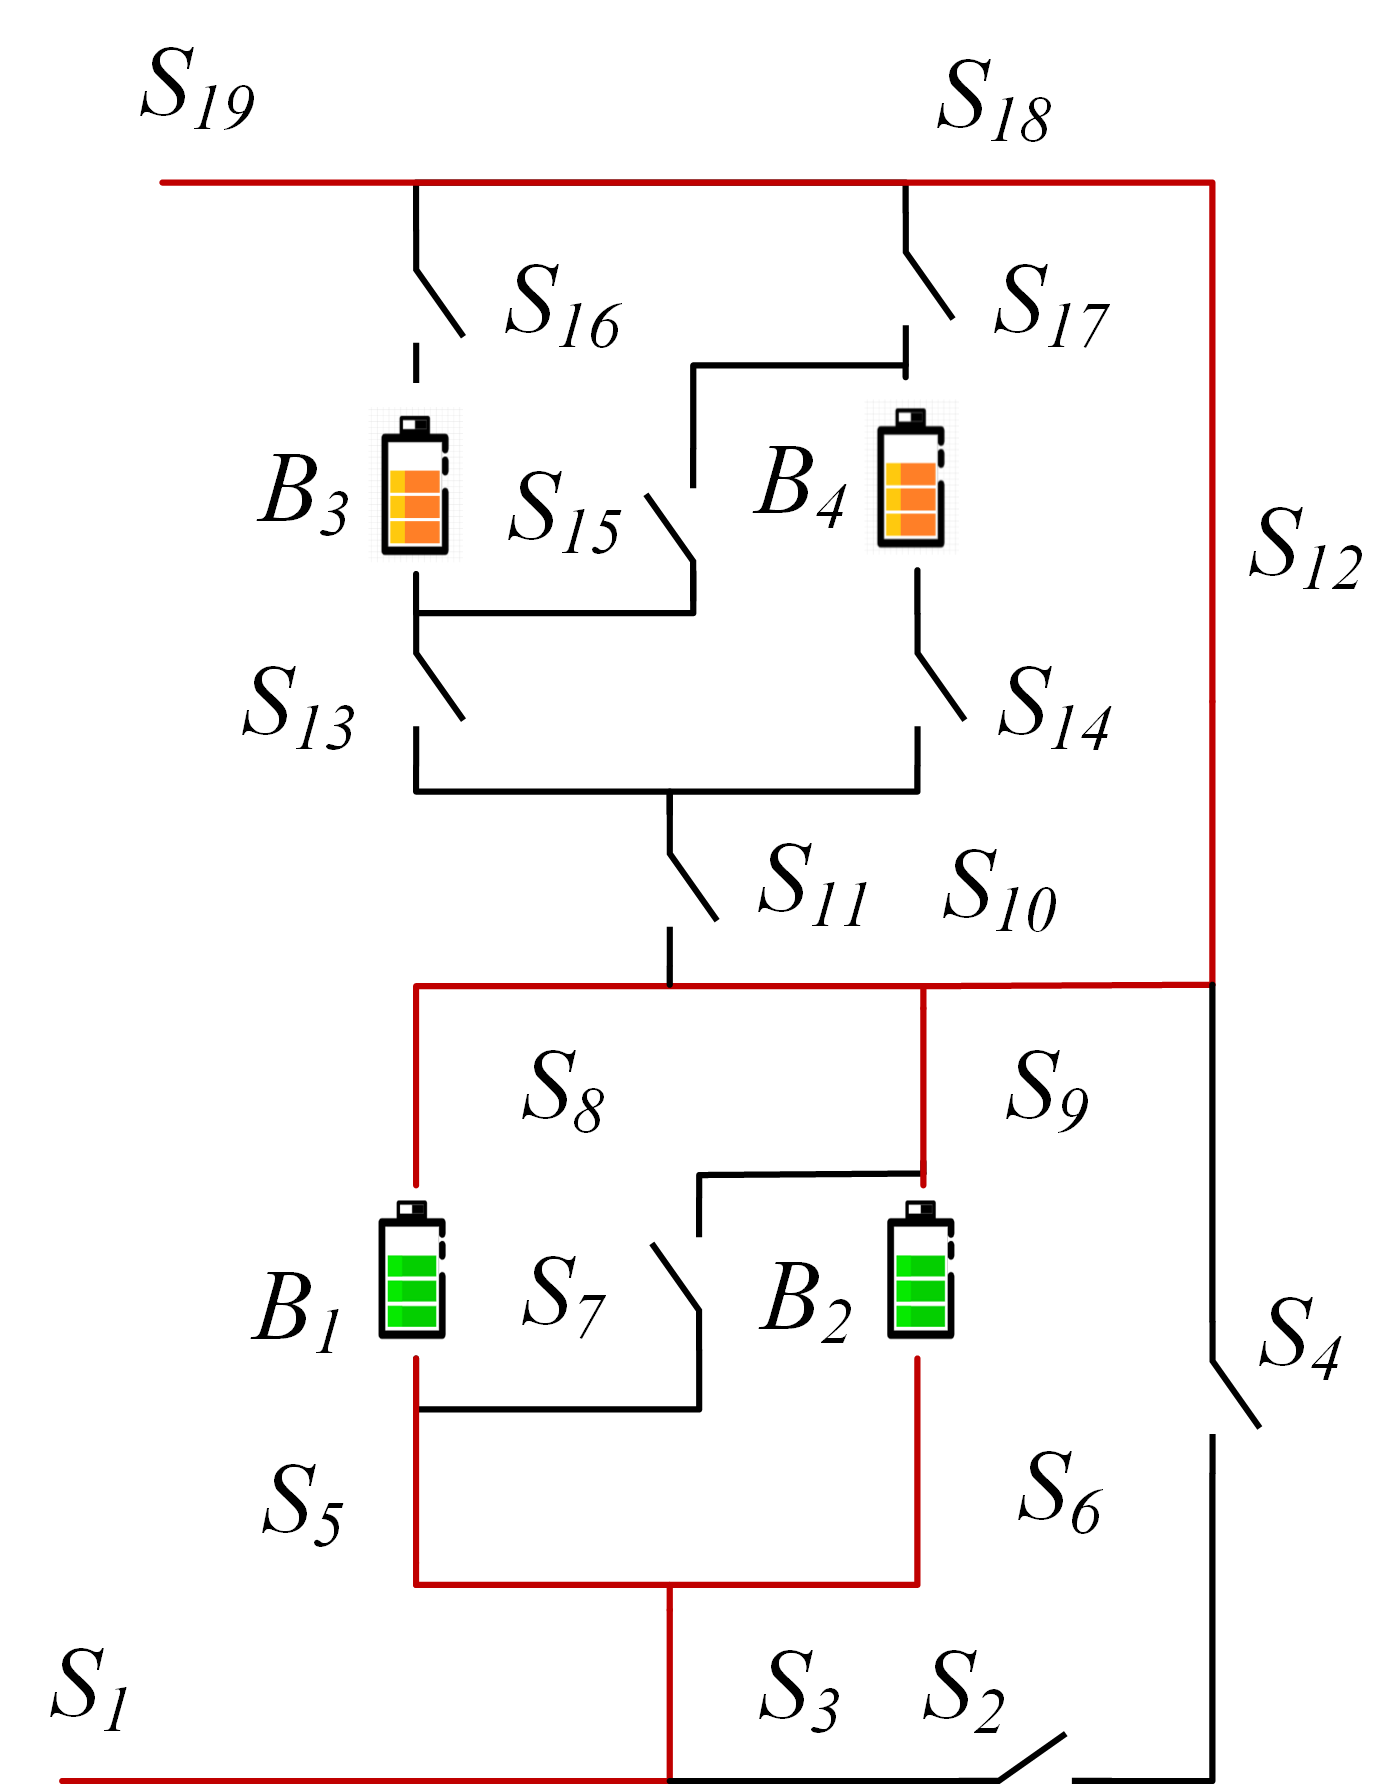
\includegraphics[width=\textwidth]{my-isolated-2b.png}
          \caption{}
          \label{fig:my-isolated-2b}
      \end{subfigure}
      \\
      \begin{subfigure}[b]{0.31\textwidth}
          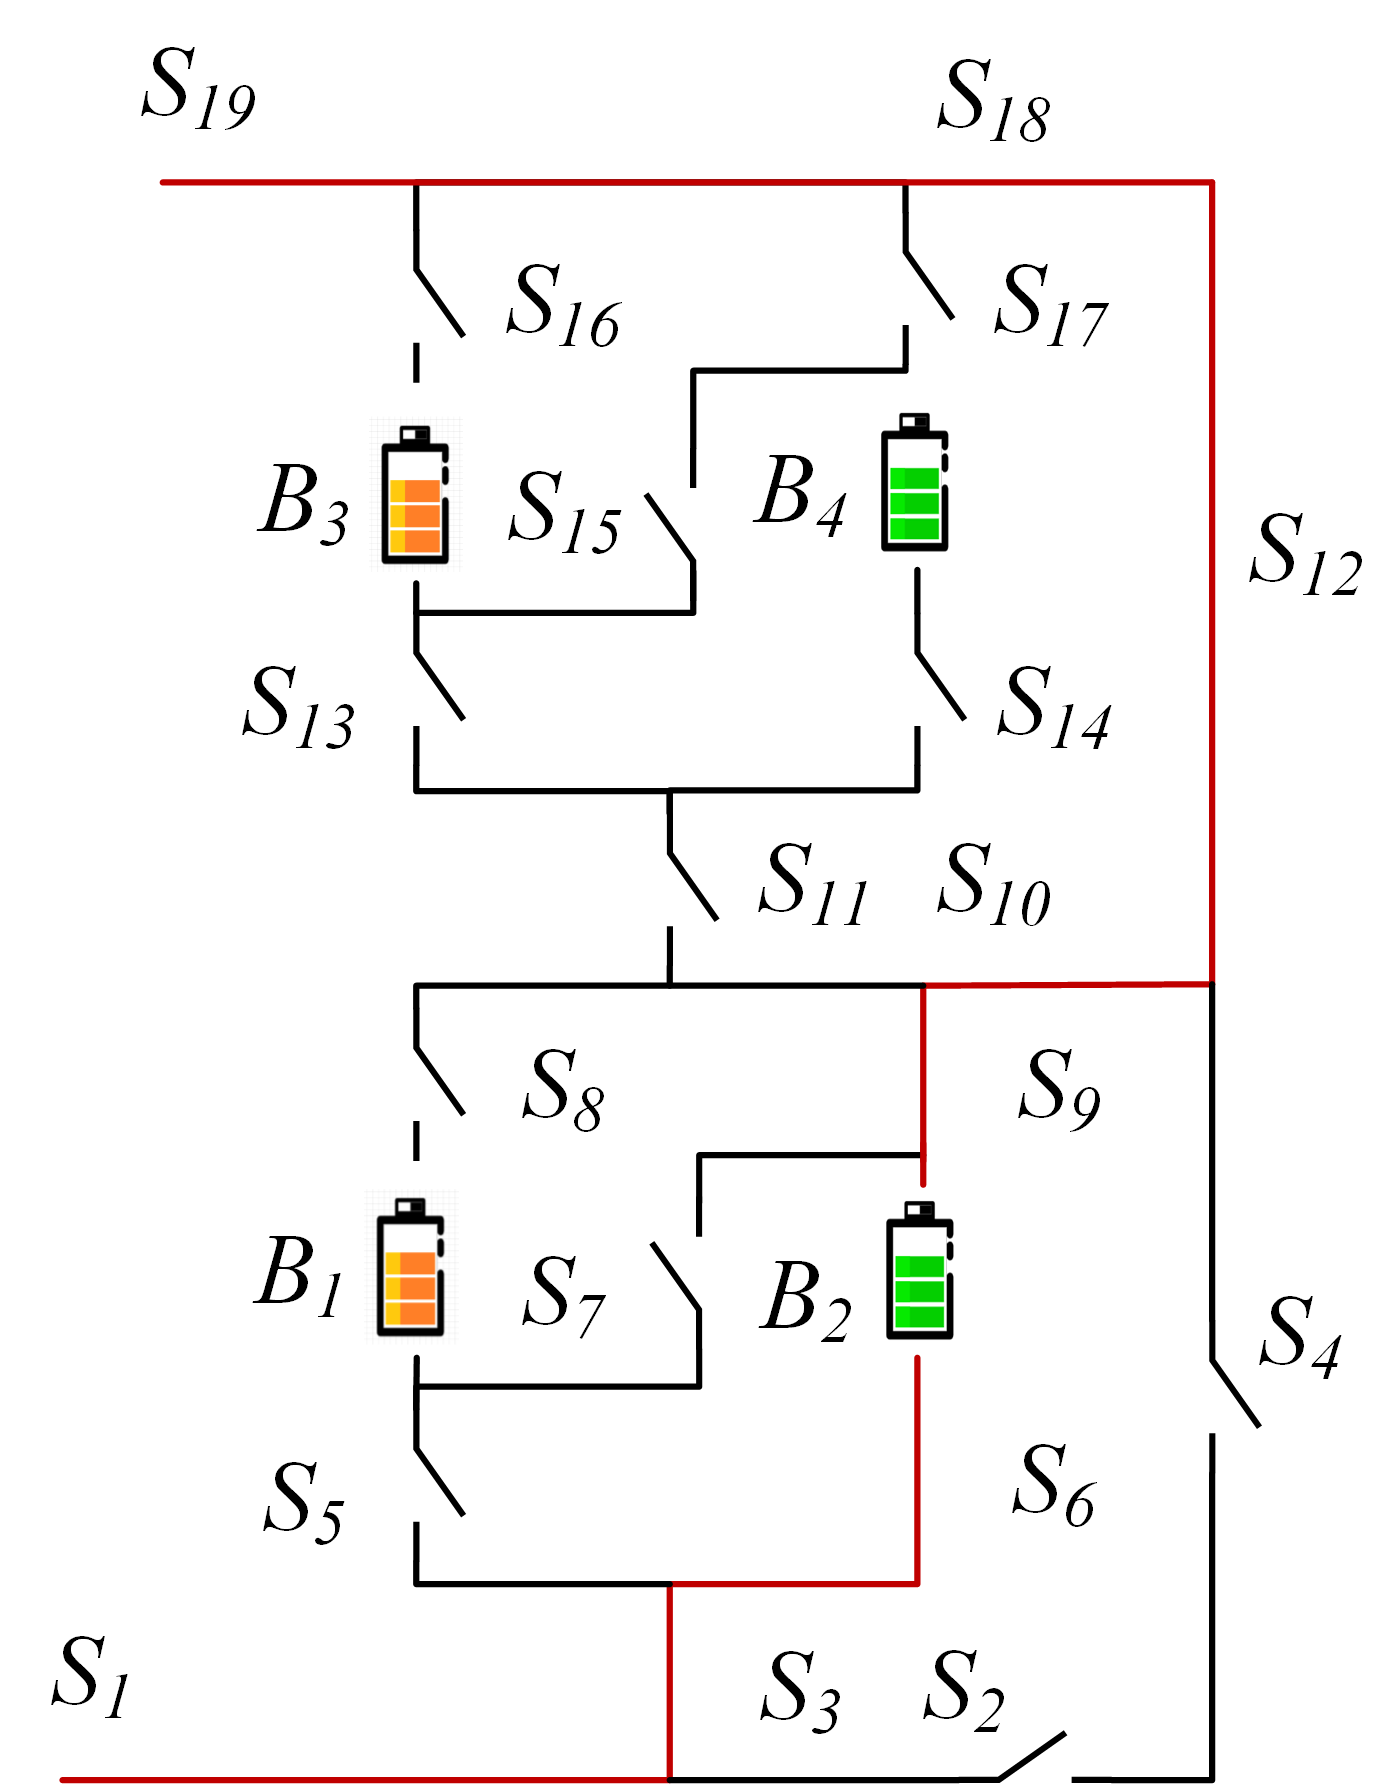
\includegraphics[width=\textwidth]{my-isolated-2w.png}
          \caption{}
          \label{fig:my-isolated-2w}
      \end{subfigure}
      \hspace{0.02\textwidth}
      \begin{subfigure}[b]{0.31\textwidth}
          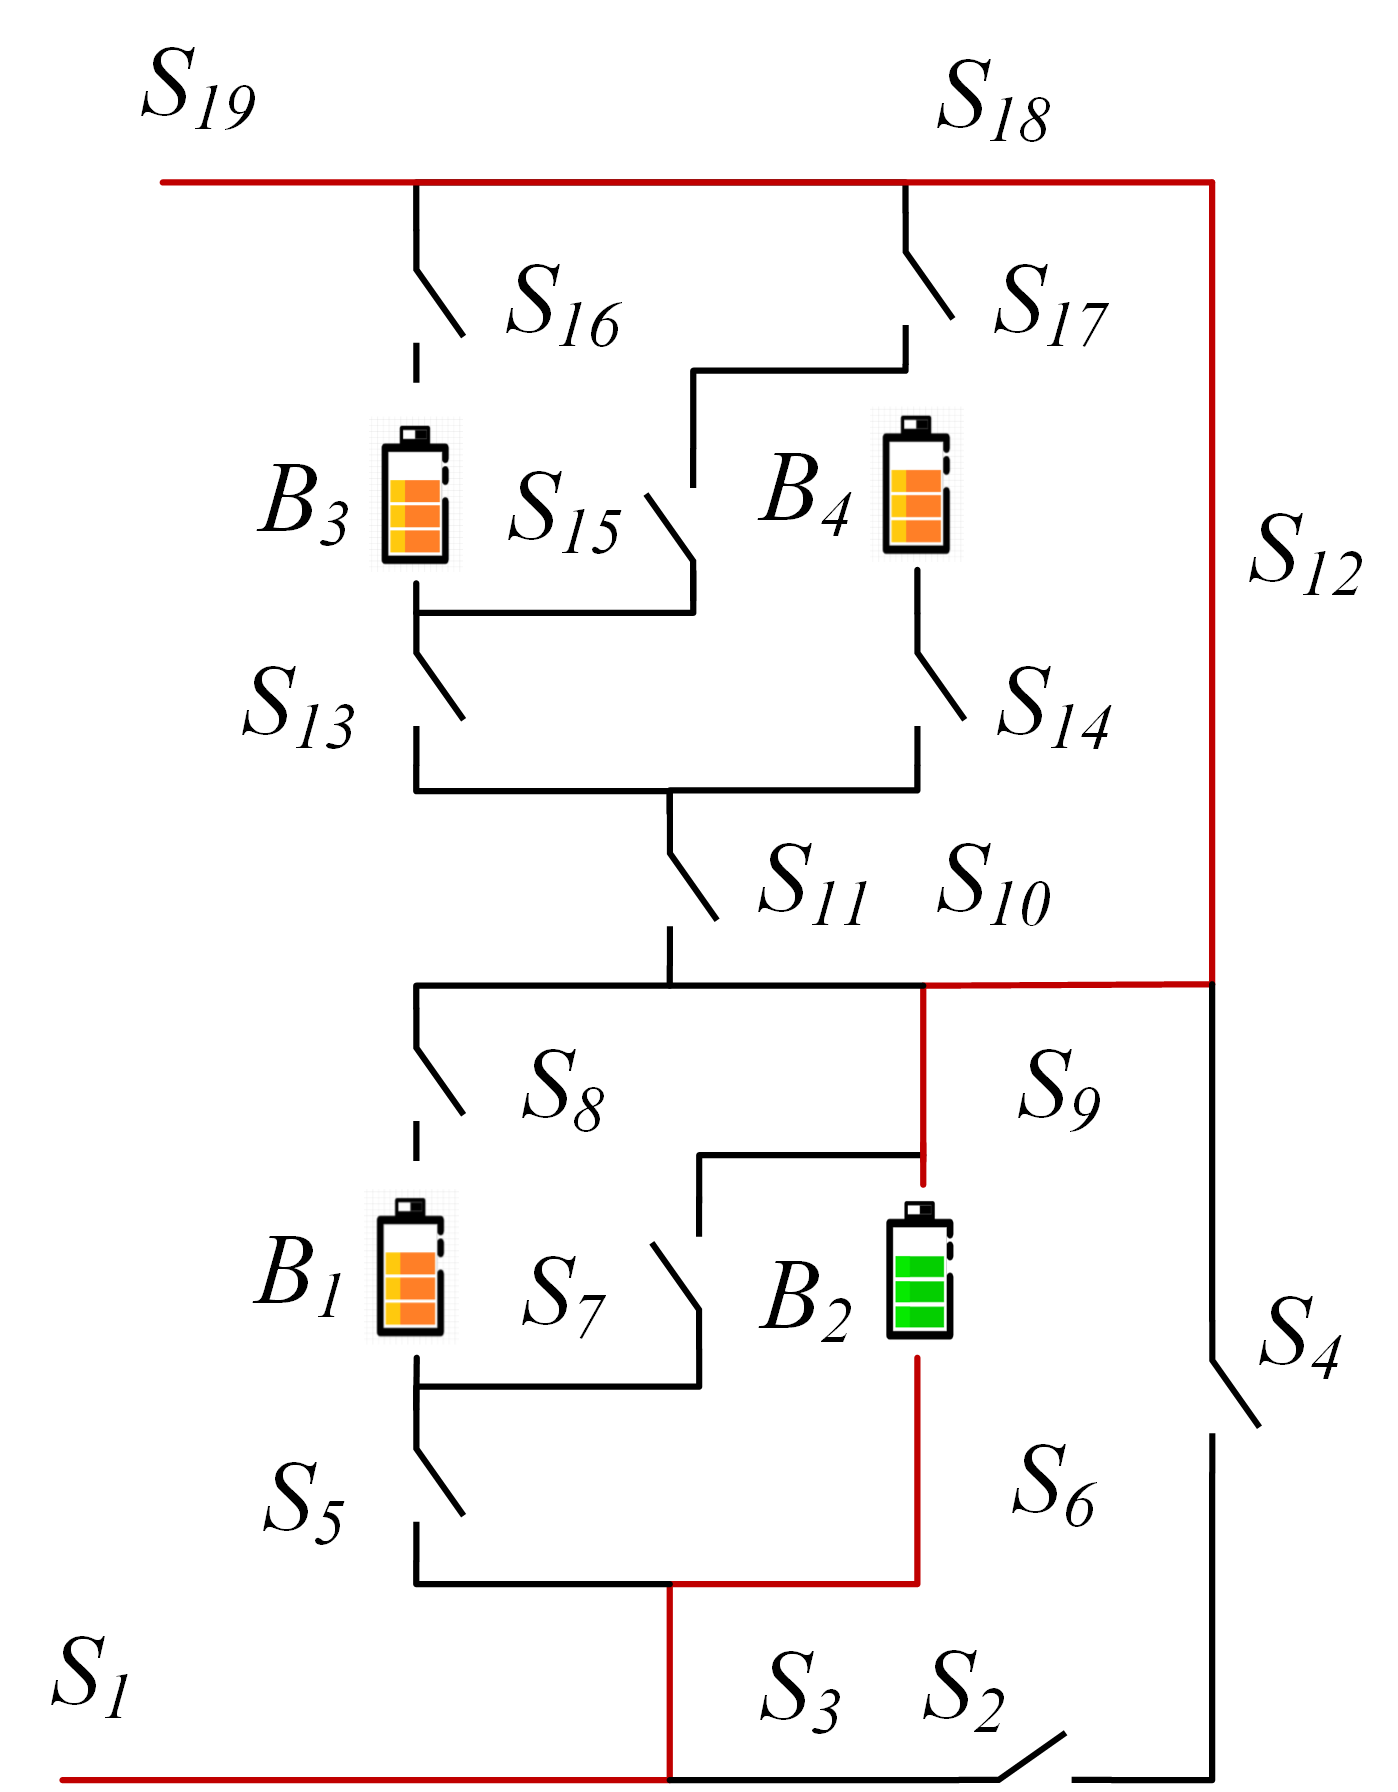
\includegraphics[width=\textwidth]{my-isolated-3.png}
          \caption{}
          \label{fig:my-isolated-3}
      \end{subfigure}
      \caption{
          The circuit states of MACs when isolating (a)one, (b)two(best case), (c)two(worst case) and (d)three batteries for the structure in Figure \ref{fig:study-stru-my}.
          }
  \end{figure}

\subsection{Discussion}

\replaced{As shown in Figure \ref{fig:all-results-my} and Table \ref{tab:study-results-my}}{In this subsection, we firstly discuss the correctness of the results presented in Figure \ref{fig:all-results-my} and Table \ref{tab:study-results-my}}.
When $B_1$ and $B_2$ or $B_3$ and $B_4$ are connected in parallel, the RBS can output the maximum current, which is $\eta=2$, i.e., twice the current output of a single battery in RBS. 
Adding more batteries to the main circuit can only form a series structure and will not improve the MAC. 
Therefore, the switches state given in Table \ref{tab:study-results-my} can make the RBS output current reach the maximum.
\added{The results of MAC obtained by brute force algorithm method is identical to the one by the greedy algorithm.}


\added{
From the literature research we have conducted, no formal report on the algorithm for MAC in RBS has been found yet.
The brute force algorithm, which goes through all possible switch states, is the most straightforward way to solve the MAC problem and is used as a benchmark for the proposed greedy algorithm.
Assuming that a RBS has $N_b$ batteries and $N_s$ switches, and the corresponding directed graph has $N$ nodes, it requires $2^{N_s}$ iterations to traverse all reconfigured structures.
The calculation for each reconfigured structure by Equations \ref{eq:I_o}-\ref{eq:eta} requires matrix inversion and matrix multiplication, with a time complexity of $O(N^3+2N^2N_b+N^2N_s+NN^2_b)$.
Therefore, the time complexity of the brute force algorithm is $O(2^{N_s}(N^3+2N^2N_b+N^2N_s+NN^2_b))$.
The greedy algorithm proposed in this paper requires find the $SP$ for each battery, which requires $N_b$ iterations.
Each $SP$ can be obtained by couple Dijkstra algorithms.
Therefore, the total time complexity of calculating all $SP$s is $O(2N_b(N_b+2N_s)\log N)$.
According to the Appendix 1, % \ref{alg:greedy},
the RBS can reconfigure $C^{N_{set}}_{N_b}$ structures by selecting $N_{set}$ batteries from $N_b$ batteries, which is $\sum^{N_b}_{N_{set}=1}C^{N_{set}}_{N_b}/N_b \approx 2^{N_b}/N_b$ on average.
Hence, with bisection method, the time complexity of the greedy algorithm is $O(2^{N_b}/N_b(N^3+2N^2N_b+N^2N_s+NN^2_b)\log N_b+2N_b(N_b+2N_s)\log N)$, i.e., $O(2^{N_b}/N_b(N^3+2N^2N_b+N^2N_s+NN^2_b)\log N_b)$.
Based on currently proposed RBS structures\cite{ciNovelDesignAdaptive2007,alahmadBatterySwitchArray2008,kimDependableEfficientScalable2010b,kimBalancedReconfigurationStorage2011a,taesickimSeriesconnectedSelfreconfigurableMulticell2012a,6843711}, the number of batteries $N_b$, switches $N_s$, and nodes $N$ have the following quantitative relationships: $N_s \approx (3\sim 5)N_b$, $N \approx N_s$. 
After simplifying, the time complexity of the greedy algorithm is $O(2^{N_b}N_s^2\log N_b)$, while it is $O(2^{N_s}N_s^3)$ for brute force algorithm.
Therefore, it is reasonable to believe that as the size of the RBS increases, especially the number of the switches, the greedy algorithm will have an advantage over the algorithm that goes through all reconfigured structures.
This can be confirmed from the number of structures required for MAC determination in the previous subsection. 
Compared to the brute force algorithm, the efficiency of the method based on the greedy algorithm has been improved by 3000 to 75000 times, which is theoretically $N_s 2^{N_s - N_b} \log N_b$ times according to the above time complexity analysis.
Among the three RBS structures, the highest is the RBS structure with 19 switches (Figure \ref{fig:study-stru-my}).
This benefit from two key points:
(1) The $SP$s guide the RBS to reconfigure reasonable structures, rather than blindly going through all possible structures. This reduces the factor in complexity from $2^{N_s}$ to $2^{N_b}$, which is the main reason for the improvement in efficiency;
(2) The bisection method further accelerates this process.
However, the greedy algorithm proposed in this paper still contains exponential terms in the time complexity, which means it may not be able to handle extremely large-scale RBS structures.
}


It is important to note that \deleted{when solving for MAC,} $\eta$ is used as the objective function instead of $I_o$ \added{in solving MAC}. 
This choice makes the result of MAC more reasonable. 
As shown in Table \ref{tab:study-results-my}, $I_o$ and $\bm{I}_b$ are functions of $R_o$, $u_b$, and $r_b$. 
\replaced{However, when}{If} $I_o$ \replaced{was}{were} used as the objective function, even for the same RBS structure, the MAC \replaced{solution}{result} and corresponding switches state could change due to different external electrical appliances.
It would increase the difficulty and uncertainty in RBS structure design. 
\replaced{In order to eliminate the influences of such a problem, $\eta$, which is the ratio of $I_o$ and $\max\bm{I}_b$, is adopted as the objective function in our research.}{In contrast, by using $\eta$ as the objective function, which is defined as the ratio of $I_o$ and $\max\bm{I}_b$, the influence of these factors on the results can be eliminated.}
$\eta$ solely reflects the maximum output current capability of the RBS structure. 
Assuming that the maximum allowed current of batteries in the RBS is $I_m$, the maximum output current of the RBS structure can be calculated as $\eta I_m$ by determining the $\eta$ of the structure. 
\deleted{Therefore, compared to $I_o$, $\eta$ is more suitable for structure design.}


The method proposed in this paper is significant for the design of \deleted{next-generation} RBSs in the following aspects.
Most of the currently proposed RBS structures\cite{ciNovelDesignAdaptive2007,alahmadBatterySwitchArray2008,kimDependableEfficientScalable2010b,kimBalancedReconfigurationStorage2011a,taesickimSeriesconnectedSelfreconfigurableMulticell2012a,6843711} exhibit simple topological characteristics, and the calculation of MACs is relatively straightforward, even intuitive.
However, these simple structures do not always fully satisfy the requirements of complex applications, such as dynamically adapting the circuit to variable and random operating conditions, and actively equalizing differences among the batteries in the RBS.
Moreover, \replaced{isolation of}{isolating} the batteries disrupts the original regularity and symmetry of the topology, which complicates the otherwise simple structure, and the maximum output current of the system becomes more challenging to obtain.
\replaced{On the contrary}{Owing to the advantages of pervasiveness and automation}, the proposed method can be employed to calculate the MAC of arbitrary RBS structures, \replaced{especially for these above complex and flexible RBS structures}{which helps to address the aforementioned issues and paves the way for more complex and flexible RBS structure design}.


To illustrate this point, the MACs of \deleted{the} three RBS structures mentioned above are calculated after \replaced{one and more}{the} batteries are isolated, as shown in Table \ref{tab:isolated_mac}. 
Specifically, for the structure presented in Figure \ref{fig:study-stru-my}, the corresponding circuit states of MACs \replaced{of}{when} isolating \replaced{one to three}{different numbers of} batteries are depicted in Figures \ref{fig:my-isolated-1}-\ref{fig:my-isolated-3}. 
This structure has two cases of isolating two batteries: 
one is to isolate two batteries within the same substructure (Figure \ref{fig:my-isolated-2b}), in which case $\eta=2$; the other is to isolate one battery in each of the two substructures (Figure \ref{fig:my-isolated-2w}), in which case $\eta=1$. 
From the results \added{shown in Figure \ref{fig:my-isolated-1}-\ref{fig:my-isolated-3}}, it can be observed that the proposed method provides reasonable outcomes for isolating batteries with any number and position.


Furthermore, the \deleted{performance of} output current for the three RBS \replaced{with isolated}{when isolating} batteries is also shown in Table \ref{tab:isolated_mac}. 
For the structure proposed by Lawson et al., the MAC \replaced{is independent on the number of isolated batteries}{remains the same as that without isolated battery cells, i.e., $\eta=1$, when the number of isolated battery cells increases, until all the cells in the RBS are isolated}.
\added{However,} \replaced{f}{F}or Visairo's structure, the MAC decreases \replaced{with the increasing number of isolated batteries}{as the number of isolated battery cells increases, until $\eta=0$}. 
\replaced{Nevertherless}{In contrast}, the MAC of the structure proposed in this work is positioned between \replaced{these above}{the} two structures. 
This indicates that the structure proposed in this paper, compared to Lawson's structure, has a larger MAC under the same number of batteries, \replaced{and exhibits}{which means} a wider output current regulation range. 
\deleted{On the other hand, by simply changing the states of $S_2$, $S_4$, $S_{11}$, and $S_{12}$ in the conversion structure, this structure can address the majority of battery isolation scenarios, whereas Visairo's structure requires specific battery targeting and switch control.}
\deleted{In summary, the structure proposed in this paper has the advantages of both Lawson's and Visairo's structures.}

\section{Conclusion}

This paper proposes a pervasive and automatical method for computing the MAC of \replaced{a}{the} given RBS \added{efficiently}.
\added{
The method is implemented by a greedy algorithm combined with a directed graph model which considers the voltage, internal resistance, and maximum allowable current of the batteries, as well as the external load.
The main advantage of this method is its ability to calculate the MAC of RBSs with arbitrary structures.
Even in the scenarios with random isolated batteries, the method remains effective.
Compared with the brute force algorithm, the proposed method has higher computational efficiency under the same calculation results.
This is achieved by two key points when constructing the greedy algorithm: 
(1) Calculate the shortest path of each battery by Dijkstra algorithm to obtain the $SP$ of each battery; 
(2) determine the maximum number of available batteries by bisection method to reduce the computational complexity.
This method helps to fully tap the current output potential of the RBS, guide the RBS structure design and optimization in the design stage, and assist in evaluating the current overload risk of the system in practical applications.
}
\deleted{The method is implemented by a greedy algorithm combined with a directed graph model , whose effectiveness is tested on a novel and complex RBS structure.
The method remains effective for the application scenario of RBS battery isolation and demonstrates that the novel structure has the advantage on flexible output current and convenient battery isolation.
Future research could focus on developing new indictors to evaluate the performance of the RBS with the currents and voltages obtained by the method, as well as modifying the equivalent model of the battery to allow for more accurate simulations of the RBS, including transient analysis.}

\section{Appendix} 

% \begin{algorithm}
%     \caption{Get the max available currents of a certain RBS}\label{alg:greedy}
%     \KwData{Directed graph model $G(V,E)$ of the RBS}
%     \KwResult{$\max \eta$}
%     \For{$i \in E_b$}{
%         $P_i \leftarrow \{path| \text{starts at $v_1$ and ends at $v_n$} \}$\;
%         $SP_i \leftarrow p_i \text{ which has the minimum}~\omega(p_i)~\text{among all}~p_i \in P_i. $
%     }
%     get $\bm{A}$ by Equation \ref{eq:A}\;
%     \While{not yet determine $\max \eta$ }
%     {
%         $N_{set} \leftarrow \text{number of setected $SP$s calculated by dichotomy}$\;
%         $C_b    \leftarrow \text{set of all combinations of $N_{set} $~batteries from $N_b$}$\;
%         \For{$c_b \in C_b$}{
%             $\bm{x}_s \leftarrow \text{list of all switches' state: $x_s[j]=1$ if $ j \in \bigcup_{i\in c_b}SP_i $ else 0}$\;
%             $\bm{X} \leftarrow diag[1,1,\cdots,1,\bm{x}_s] $\;
%             get $\bm{Y}_n$ by Equation \ref{eq:Yn}\;
%             \eIf{$\bm{Y}_n$ is invertible}{
%               \added{pass}
%             }{construct an effective solution}
%             get $I_o$ by Equation \ref{eq:I_o}\;
%             get $\bm{I}_b$ by Equation \ref{eq:I_b}\;
%             \eIf{$\max(\bm{I}_b)\leq I_m$}{
%                 $\eta \leftarrow I_o/\max(\bm{I}_b)$\;
%             }{break}
%         }
%     }
% \end{algorithm}
\begin{figure}[htbp]
    \centering
    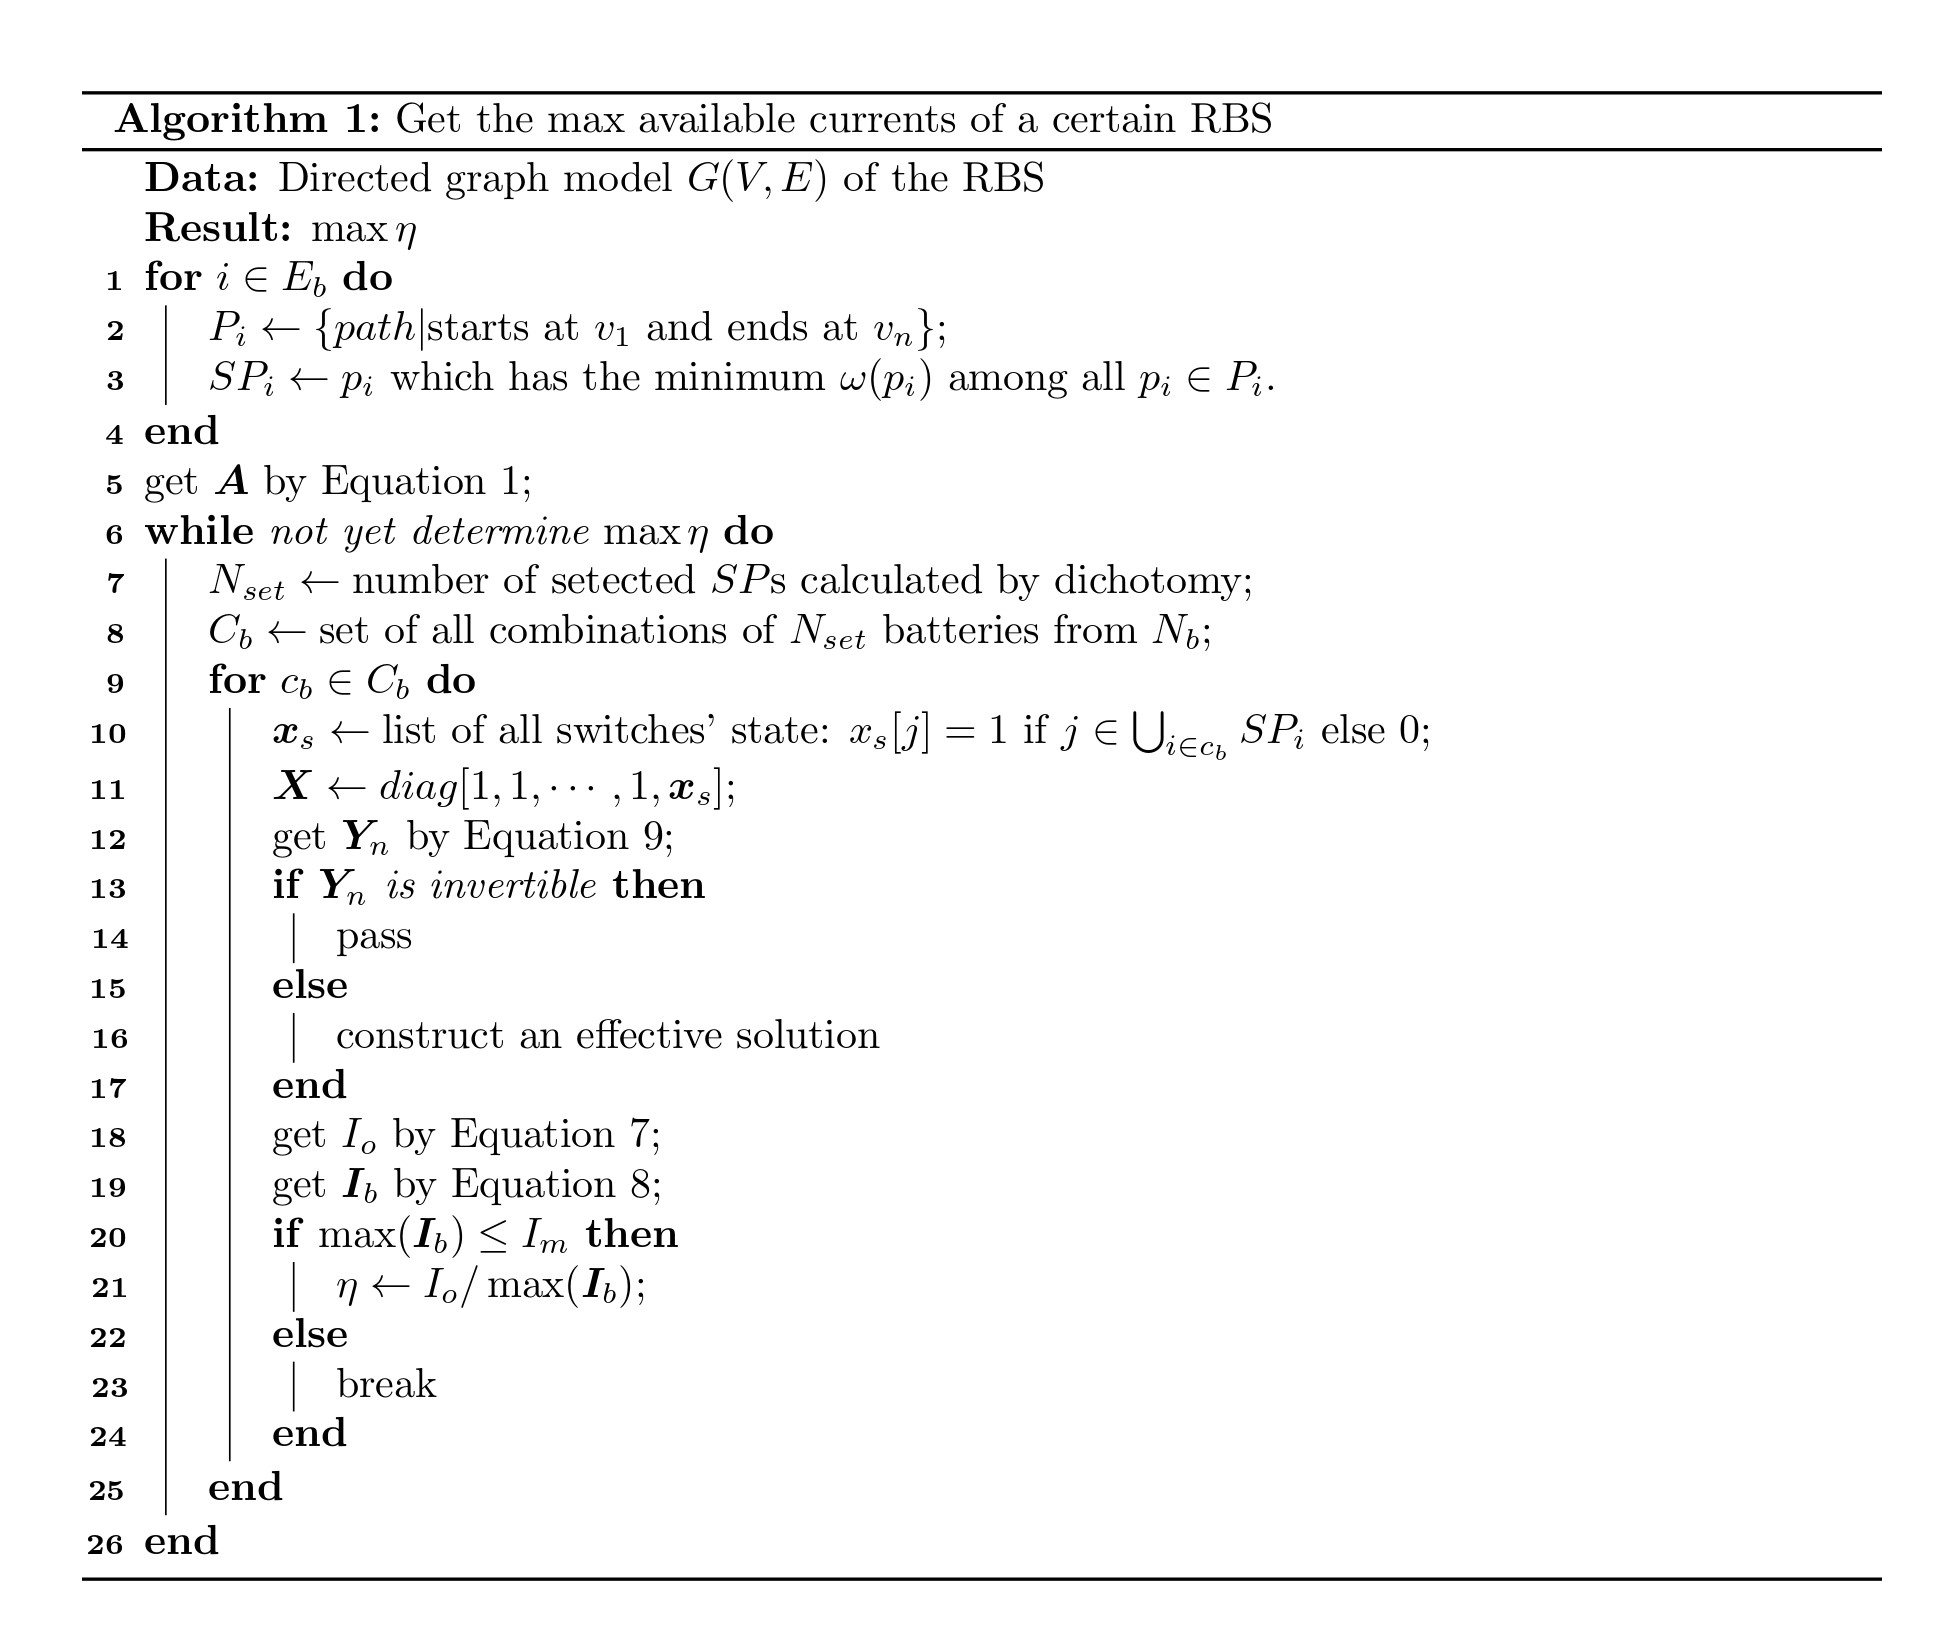
\includegraphics[width=\textwidth]{algorithm.jpg}
\end{figure}

% 
% \section*{Acknowledgments}
% 
% \subsection*{Author Contributions} 
% 
% B. Xu conceived the main idea, formulated the overarching research goals and aims, designed the algorithm, and reviewed and revised the manuscript.
% G. Hua developed and analyzed the model, implemented the code and supporting algorithms, and wrote the initial draft.
% C. Qian provided critical review, commentary, and revisions.
% Q. Xia contributed to shaping the research, analysis, and manuscript.
% B. Sun conducted the research and investigation process.
% Y. Ren secured the funding and supervised the project.
% Z. Wang verified the results and provided necessary resources.
% 
% \subsection*{Funding}
% 
% This work was supported by the National Natural Science Foundation of China (NSFC, No.52075028).
% 
% \subsection*{Conflicts of Interest}
% 
% The authors declare that there is no conflict of interest regarding the publication of this article.
% 
% \subsection*{Data Availability}
% 
% This work does not require any data to be declared or publicly disclosed.

% \bibliographystyle{nejm}
% \bibliography{sst_main}

% \printbibliography

\end{document}
